\documentclass{book}
\usepackage[a4paper,top=2.5cm,bottom=2.5cm,left=2.5cm,right=2.5cm]{geometry}
\usepackage{makeidx}
\usepackage{natbib}
\usepackage{graphicx}
\usepackage{multicol}
\usepackage{float}
\usepackage{listings}
\usepackage{color}
\usepackage{ifthen}
\usepackage[table]{xcolor}
\usepackage{textcomp}
\usepackage{alltt}
\usepackage{ifpdf}
\ifpdf
\usepackage[pdftex,
            pagebackref=true,
            colorlinks=true,
            linkcolor=blue,
            unicode
           ]{hyperref}
\else
\usepackage[ps2pdf,
            pagebackref=true,
            colorlinks=true,
            linkcolor=blue,
            unicode
           ]{hyperref}
\usepackage{pspicture}
\fi
\usepackage[utf8]{inputenc}
\usepackage{mathptmx}
\usepackage[scaled=.90]{helvet}
\usepackage{courier}
\usepackage{sectsty}
\usepackage{amssymb}
\usepackage[titles]{tocloft}
\usepackage{doxygen}
\lstset{language=C++,inputencoding=utf8,basicstyle=\footnotesize,breaklines=true,breakatwhitespace=true,tabsize=8,numbers=left }
\makeindex
\setcounter{tocdepth}{3}
\renewcommand{\footrulewidth}{0.4pt}
\renewcommand{\familydefault}{\sfdefault}
\hfuzz=15pt
\setlength{\emergencystretch}{15pt}
\hbadness=750
\tolerance=750
\begin{document}
\hypersetup{pageanchor=false,citecolor=blue}
\begin{titlepage}
\vspace*{7cm}
\begin{center}
{\Large Real-\/\-Time Embedded Autonomous Car }\\
\vspace*{1cm}
{\large Generated by Doxygen 1.8.1.2}\\
\vspace*{0.5cm}
{\small Sun May 5 2013 16:39:13}\\
\end{center}
\end{titlepage}
\clearemptydoublepage
\pagenumbering{roman}
\tableofcontents
\clearemptydoublepage
\pagenumbering{arabic}
\hypersetup{pageanchor=true,citecolor=blue}
\chapter{realtime}
\label{md_README}
\hypertarget{md_README}{}
realtime project 
\chapter{Module Index}
\section{Modules}
Here is a list of all modules\-:\begin{DoxyCompactList}
\item \contentsline{section}{Subsystem Numbers}{\pageref{group__subsys__nums}}{}
\item \contentsline{section}{Steering Commands}{\pageref{group__steering__commands}}{}
\item \contentsline{section}{Motor Commands}{\pageref{group__motor__commands}}{}
\item \contentsline{section}{Compass Commands}{\pageref{group__compass__commands}}{}
\item \contentsline{section}{G\-P\-S Commands}{\pageref{group__gps__commands}}{}
\item \contentsline{section}{Sonar Commands}{\pageref{group__sonar__commands}}{}
\end{DoxyCompactList}

\chapter{Class Index}
\section{Class Hierarchy}
This inheritance list is sorted roughly, but not completely, alphabetically\-:\begin{DoxyCompactList}
\item \contentsline{section}{\-\_\-\-M\-E\-S\-S\-A\-G\-E}{\pageref{struct__MESSAGE}}{}
\item \contentsline{section}{Subsystem}{\pageref{classSubsystem}}{}
\begin{DoxyCompactList}
\item \contentsline{section}{Actuator}{\pageref{classActuator}}{}
\begin{DoxyCompactList}
\item \contentsline{section}{Motor}{\pageref{classMotor}}{}
\item \contentsline{section}{Steering}{\pageref{classSteering}}{}
\end{DoxyCompactList}
\item \contentsline{section}{Sensor}{\pageref{classSensor}}{}
\begin{DoxyCompactList}
\item \contentsline{section}{Compass}{\pageref{classCompass}}{}
\item \contentsline{section}{G\-P\-S}{\pageref{classGPS}}{}
\item \contentsline{section}{Sonar}{\pageref{classSonar}}{}
\end{DoxyCompactList}
\end{DoxyCompactList}
\item \contentsline{section}{System\-Control}{\pageref{classSystemControl}}{}
\end{DoxyCompactList}

\chapter{Class Index}
\section{Class List}
Here are the classes, structs, unions and interfaces with brief descriptions\-:\begin{DoxyCompactList}
\item\contentsline{section}{\hyperlink{struct__ADC__DATA}{\-\_\-\-A\-D\-C\-\_\-\-D\-A\-T\-A} }{\pageref{struct__ADC__DATA}}{}
\item\contentsline{section}{\hyperlink{struct__MESSAGE}{\-\_\-\-M\-E\-S\-S\-A\-G\-E} \\*Defines the structure of a message to be sent to a subsystem }{\pageref{struct__MESSAGE}}{}
\item\contentsline{section}{\hyperlink{classActuator}{Actuator} \\*\hyperlink{classActuator}{Actuator} class manages actuator tasks }{\pageref{classActuator}}{}
\item\contentsline{section}{\hyperlink{classADC}{A\-D\-C} \\*\hyperlink{classCompass}{Compass} data collection and analysis }{\pageref{classADC}}{}
\item\contentsline{section}{\hyperlink{classCompass}{Compass} \\*\hyperlink{classCompass}{Compass} data collection and analysis }{\pageref{classCompass}}{}
\item\contentsline{section}{\hyperlink{classGPS}{G\-P\-S} \\*\hyperlink{classGPS}{G\-P\-S} data collection and analysis }{\pageref{classGPS}}{}
\item\contentsline{section}{\hyperlink{classGPS_1_1GPSWayPoint}{G\-P\-S\-::\-G\-P\-S\-Way\-Point} \\*Stores \hyperlink{classGPS}{G\-P\-S} Way\-Points as a linked list }{\pageref{classGPS_1_1GPSWayPoint}}{}
\item\contentsline{section}{\hyperlink{classGPS_1_1LatLon}{G\-P\-S\-::\-Lat\-Lon} \\*Structure that hold latitude and longitude }{\pageref{classGPS_1_1LatLon}}{}
\item\contentsline{section}{\hyperlink{classMotor}{Motor} \\*\hyperlink{classMotor}{Motor} control }{\pageref{classMotor}}{}
\item\contentsline{section}{\hyperlink{classSensor}{Sensor} \\*\hyperlink{classSensor}{Sensor} class manages sensor tasks }{\pageref{classSensor}}{}
\item\contentsline{section}{\hyperlink{classSonar}{Sonar} \\*\hyperlink{classSonar}{Sonar} data collection and analysis }{\pageref{classSonar}}{}
\item\contentsline{section}{\hyperlink{classSteering}{Steering} \\*\hyperlink{classSteering}{Steering} control }{\pageref{classSteering}}{}
\item\contentsline{section}{\hyperlink{classsubsys__timing}{subsys\-\_\-timing} }{\pageref{classsubsys__timing}}{}
\item\contentsline{section}{\hyperlink{classSubsystem}{Subsystem} \\*Defines the basic properties shared by all subsystems }{\pageref{classSubsystem}}{}
\item\contentsline{section}{\hyperlink{classsystem__logger}{system\-\_\-logger} }{\pageref{classsystem__logger}}{}
\item\contentsline{section}{\hyperlink{classSystemControl}{System\-Control} \\*System control is the central controller }{\pageref{classSystemControl}}{}
\item\contentsline{section}{\hyperlink{classtiming__analysis}{timing\-\_\-analysis} }{\pageref{classtiming__analysis}}{}
\item\contentsline{section}{\hyperlink{classCompass_1_1Vector3d}{Compass\-::\-Vector3d} }{\pageref{classCompass_1_1Vector3d}}{}
\end{DoxyCompactList}

\chapter{File Index}
\section{File List}
Here is a list of all documented files with brief descriptions\-:\begin{DoxyCompactList}
\item\contentsline{section}{/home/keith/realtime/{\bfseries Actuator.\-h} }{\pageref{Actuator_8h}}{}
\item\contentsline{section}{/home/keith/realtime/{\bfseries A\-D\-C.\-h} }{\pageref{ADC_8h}}{}
\item\contentsline{section}{/home/keith/realtime/{\bfseries Compass.\-h} }{\pageref{Compass_8h}}{}
\item\contentsline{section}{/home/keith/realtime/{\bfseries G\-P\-S.\-h} }{\pageref{GPS_8h}}{}
\item\contentsline{section}{/home/keith/realtime/{\bfseries Motor.\-h} }{\pageref{Motor_8h}}{}
\item\contentsline{section}{/home/keith/realtime/{\bfseries M\-Q\-\_\-\-P\-A\-R\-A\-M\-S.\-h} }{\pageref{MQ__PARAMS_8h}}{}
\item\contentsline{section}{/home/keith/realtime/{\bfseries Sensor.\-h} }{\pageref{Sensor_8h}}{}
\item\contentsline{section}{/home/keith/realtime/{\bfseries shirtt.\-h} }{\pageref{shirtt_8h}}{}
\item\contentsline{section}{/home/keith/realtime/{\bfseries Sonar.\-h} }{\pageref{Sonar_8h}}{}
\item\contentsline{section}{/home/keith/realtime/{\bfseries Steering.\-h} }{\pageref{Steering_8h}}{}
\item\contentsline{section}{/home/keith/realtime/\hyperlink{SUBSYS__COMMANDS_8h}{S\-U\-B\-S\-Y\-S\-\_\-\-C\-O\-M\-M\-A\-N\-D\-S.\-h} }{\pageref{SUBSYS__COMMANDS_8h}}{}
\item\contentsline{section}{/home/keith/realtime/{\bfseries subsys\-\_\-timing.\-h} }{\pageref{subsys__timing_8h}}{}
\item\contentsline{section}{/home/keith/realtime/{\bfseries Subsystem.\-h} }{\pageref{Subsystem_8h}}{}
\item\contentsline{section}{/home/keith/realtime/{\bfseries system\-\_\-logger.\-h} }{\pageref{system__logger_8h}}{}
\item\contentsline{section}{/home/keith/realtime/{\bfseries System\-Control.\-h} }{\pageref{SystemControl_8h}}{}
\item\contentsline{section}{/home/keith/realtime/{\bfseries T\-A\-S\-K\-\_\-\-N\-U\-M\-B\-E\-R\-S.\-h} }{\pageref{TASK__NUMBERS_8h}}{}
\item\contentsline{section}{/home/keith/realtime/{\bfseries timing\-\_\-analysis.\-h} }{\pageref{timing__analysis_8h}}{}
\end{DoxyCompactList}

\chapter{Module Documentation}
\hypertarget{group__subsys__nums}{\section{Subsystem Numbers}
\label{group__subsys__nums}\index{Subsystem Numbers@{Subsystem Numbers}}
}
\subsection*{Macros}
\begin{DoxyCompactItemize}
\item 
\#define \hyperlink{group__subsys__nums_ga468920c27e6f462f4319229cda832476}{S\-U\-B\-S\-Y\-S\-\_\-\-G\-P\-S}~0
\item 
\#define \hyperlink{group__subsys__nums_ga7476b8f22f1670fcf89da75d9fe3b643}{S\-U\-B\-S\-Y\-S\-\_\-\-C\-O\-M\-P\-A\-S\-S}~1
\item 
\#define \hyperlink{group__subsys__nums_ga3ce4f17430989c1b4d5b0ae9ddb38df8}{S\-U\-B\-S\-Y\-S\-\_\-\-S\-O\-N\-A\-R}~2
\item 
\#define \hyperlink{group__subsys__nums_gaf957c814784b521302308d9de3fe07d1}{S\-U\-B\-S\-Y\-S\-\_\-\-M\-O\-T\-O\-R}~3
\item 
\#define \hyperlink{group__subsys__nums_ga8c00ac0932359e608b0870b1cfa7b7dc}{S\-U\-B\-S\-Y\-S\-\_\-\-S\-T\-E\-E\-R\-I\-N\-G}~4
\item 
\#define \hyperlink{group__subsys__nums_ga7ab9ade0a6a5934eb6ad244e1130929f}{S\-U\-B\-S\-Y\-S\-\_\-\-C\-A\-M\-E\-R\-A}~5
\item 
\#define \hyperlink{group__subsys__nums_gad914679f013f117ec7470f75fee6149a}{N\-U\-M\-\_\-\-S\-U\-B\-S\-Y\-S\-T\-E\-M\-S}~5
\end{DoxyCompactItemize}


\subsection{Detailed Description}
Numbers assigned to each subsystem used for unique identification by the messaging system. 

\subsection{Macro Definition Documentation}
\hypertarget{group__subsys__nums_gad914679f013f117ec7470f75fee6149a}{\index{Subsystem Numbers@{Subsystem Numbers}!N\-U\-M\-\_\-\-S\-U\-B\-S\-Y\-S\-T\-E\-M\-S@{N\-U\-M\-\_\-\-S\-U\-B\-S\-Y\-S\-T\-E\-M\-S}}
\index{N\-U\-M\-\_\-\-S\-U\-B\-S\-Y\-S\-T\-E\-M\-S@{N\-U\-M\-\_\-\-S\-U\-B\-S\-Y\-S\-T\-E\-M\-S}!Subsystem Numbers@{Subsystem Numbers}}
\subsubsection[{N\-U\-M\-\_\-\-S\-U\-B\-S\-Y\-S\-T\-E\-M\-S}]{\setlength{\rightskip}{0pt plus 5cm}\#define N\-U\-M\-\_\-\-S\-U\-B\-S\-Y\-S\-T\-E\-M\-S~5}}\label{group__subsys__nums_gad914679f013f117ec7470f75fee6149a}
Number of subsystems \hypertarget{group__subsys__nums_ga7ab9ade0a6a5934eb6ad244e1130929f}{\index{Subsystem Numbers@{Subsystem Numbers}!S\-U\-B\-S\-Y\-S\-\_\-\-C\-A\-M\-E\-R\-A@{S\-U\-B\-S\-Y\-S\-\_\-\-C\-A\-M\-E\-R\-A}}
\index{S\-U\-B\-S\-Y\-S\-\_\-\-C\-A\-M\-E\-R\-A@{S\-U\-B\-S\-Y\-S\-\_\-\-C\-A\-M\-E\-R\-A}!Subsystem Numbers@{Subsystem Numbers}}
\subsubsection[{S\-U\-B\-S\-Y\-S\-\_\-\-C\-A\-M\-E\-R\-A}]{\setlength{\rightskip}{0pt plus 5cm}\#define S\-U\-B\-S\-Y\-S\-\_\-\-C\-A\-M\-E\-R\-A~5}}\label{group__subsys__nums_ga7ab9ade0a6a5934eb6ad244e1130929f}
Camera \hyperlink{classSubsystem}{Subsystem} Number \hypertarget{group__subsys__nums_ga7476b8f22f1670fcf89da75d9fe3b643}{\index{Subsystem Numbers@{Subsystem Numbers}!S\-U\-B\-S\-Y\-S\-\_\-\-C\-O\-M\-P\-A\-S\-S@{S\-U\-B\-S\-Y\-S\-\_\-\-C\-O\-M\-P\-A\-S\-S}}
\index{S\-U\-B\-S\-Y\-S\-\_\-\-C\-O\-M\-P\-A\-S\-S@{S\-U\-B\-S\-Y\-S\-\_\-\-C\-O\-M\-P\-A\-S\-S}!Subsystem Numbers@{Subsystem Numbers}}
\subsubsection[{S\-U\-B\-S\-Y\-S\-\_\-\-C\-O\-M\-P\-A\-S\-S}]{\setlength{\rightskip}{0pt plus 5cm}\#define S\-U\-B\-S\-Y\-S\-\_\-\-C\-O\-M\-P\-A\-S\-S~1}}\label{group__subsys__nums_ga7476b8f22f1670fcf89da75d9fe3b643}
\hyperlink{classCompass}{Compass} \hyperlink{classSubsystem}{Subsystem} Number \hypertarget{group__subsys__nums_ga468920c27e6f462f4319229cda832476}{\index{Subsystem Numbers@{Subsystem Numbers}!S\-U\-B\-S\-Y\-S\-\_\-\-G\-P\-S@{S\-U\-B\-S\-Y\-S\-\_\-\-G\-P\-S}}
\index{S\-U\-B\-S\-Y\-S\-\_\-\-G\-P\-S@{S\-U\-B\-S\-Y\-S\-\_\-\-G\-P\-S}!Subsystem Numbers@{Subsystem Numbers}}
\subsubsection[{S\-U\-B\-S\-Y\-S\-\_\-\-G\-P\-S}]{\setlength{\rightskip}{0pt plus 5cm}\#define S\-U\-B\-S\-Y\-S\-\_\-\-G\-P\-S~0}}\label{group__subsys__nums_ga468920c27e6f462f4319229cda832476}
\hyperlink{classGPS}{G\-P\-S} \hyperlink{classSubsystem}{Subsystem} Number \hypertarget{group__subsys__nums_gaf957c814784b521302308d9de3fe07d1}{\index{Subsystem Numbers@{Subsystem Numbers}!S\-U\-B\-S\-Y\-S\-\_\-\-M\-O\-T\-O\-R@{S\-U\-B\-S\-Y\-S\-\_\-\-M\-O\-T\-O\-R}}
\index{S\-U\-B\-S\-Y\-S\-\_\-\-M\-O\-T\-O\-R@{S\-U\-B\-S\-Y\-S\-\_\-\-M\-O\-T\-O\-R}!Subsystem Numbers@{Subsystem Numbers}}
\subsubsection[{S\-U\-B\-S\-Y\-S\-\_\-\-M\-O\-T\-O\-R}]{\setlength{\rightskip}{0pt plus 5cm}\#define S\-U\-B\-S\-Y\-S\-\_\-\-M\-O\-T\-O\-R~3}}\label{group__subsys__nums_gaf957c814784b521302308d9de3fe07d1}
\hyperlink{classMotor}{Motor} \hyperlink{classSubsystem}{Subsystem} Number \hypertarget{group__subsys__nums_ga3ce4f17430989c1b4d5b0ae9ddb38df8}{\index{Subsystem Numbers@{Subsystem Numbers}!S\-U\-B\-S\-Y\-S\-\_\-\-S\-O\-N\-A\-R@{S\-U\-B\-S\-Y\-S\-\_\-\-S\-O\-N\-A\-R}}
\index{S\-U\-B\-S\-Y\-S\-\_\-\-S\-O\-N\-A\-R@{S\-U\-B\-S\-Y\-S\-\_\-\-S\-O\-N\-A\-R}!Subsystem Numbers@{Subsystem Numbers}}
\subsubsection[{S\-U\-B\-S\-Y\-S\-\_\-\-S\-O\-N\-A\-R}]{\setlength{\rightskip}{0pt plus 5cm}\#define S\-U\-B\-S\-Y\-S\-\_\-\-S\-O\-N\-A\-R~2}}\label{group__subsys__nums_ga3ce4f17430989c1b4d5b0ae9ddb38df8}
\hyperlink{classSonar}{Sonar} \hyperlink{classSubsystem}{Subsystem} Number \hypertarget{group__subsys__nums_ga8c00ac0932359e608b0870b1cfa7b7dc}{\index{Subsystem Numbers@{Subsystem Numbers}!S\-U\-B\-S\-Y\-S\-\_\-\-S\-T\-E\-E\-R\-I\-N\-G@{S\-U\-B\-S\-Y\-S\-\_\-\-S\-T\-E\-E\-R\-I\-N\-G}}
\index{S\-U\-B\-S\-Y\-S\-\_\-\-S\-T\-E\-E\-R\-I\-N\-G@{S\-U\-B\-S\-Y\-S\-\_\-\-S\-T\-E\-E\-R\-I\-N\-G}!Subsystem Numbers@{Subsystem Numbers}}
\subsubsection[{S\-U\-B\-S\-Y\-S\-\_\-\-S\-T\-E\-E\-R\-I\-N\-G}]{\setlength{\rightskip}{0pt plus 5cm}\#define S\-U\-B\-S\-Y\-S\-\_\-\-S\-T\-E\-E\-R\-I\-N\-G~4}}\label{group__subsys__nums_ga8c00ac0932359e608b0870b1cfa7b7dc}
\hyperlink{classSteering}{Steering} \hyperlink{classSubsystem}{Subsystem} Number 
\hypertarget{group__steering__commands}{\section{Steering Commands}
\label{group__steering__commands}\index{Steering Commands@{Steering Commands}}
}
\subsection*{Macros}
\begin{DoxyCompactItemize}
\item 
\#define \hyperlink{group__steering__commands_ga0c1cb6fd30382725c9828e619d0d813c}{S\-T\-R\-\_\-\-H\-A\-R\-D\-\_\-\-L\-E\-F\-T}~0
\item 
\#define \hyperlink{group__steering__commands_ga9460f3ea1c94d0cbea0651cea23a6b90}{S\-T\-R\-\_\-\-H\-A\-R\-D\-\_\-\-R\-I\-G\-H\-T}~1
\item 
\#define \hyperlink{group__steering__commands_ga0bf8759a57b2161c90c56b4186545018}{S\-T\-R\-\_\-\-S\-L\-I\-G\-H\-T\-\_\-\-L\-E\-F\-T}~2
\item 
\#define \hyperlink{group__steering__commands_ga7872976a47fb31b04cb5c4328d0b3779}{S\-T\-R\-\_\-\-S\-L\-I\-G\-H\-T\-\_\-\-R\-I\-G\-H\-T}~3
\item 
\#define \hyperlink{group__steering__commands_gaea8bf1d4bcf9c8b6bfd778fb81f91eab}{S\-T\-R\-\_\-\-F\-I\-N\-E\-\_\-\-L\-E\-F\-T}~4
\item 
\#define \hyperlink{group__steering__commands_ga97aef886486d06481892129ac63b29ba}{S\-T\-R\-\_\-\-F\-I\-N\-E\-\_\-\-R\-I\-G\-H\-T}~5
\item 
\#define \hyperlink{group__steering__commands_ga85d1e93794cb6ca3f82ba6b211897ac6}{S\-T\-R\-\_\-\-S\-T\-R\-A\-I\-G\-H\-T}~6
\item 
\#define \hyperlink{group__steering__commands_ga3944f02514d51b9a5fad5def73a3d492}{S\-T\-R\-\_\-\-S\-E\-T\-\_\-\-S\-T\-E\-E\-R\-I\-N\-G}~7
\item 
\#define \hyperlink{group__steering__commands_gafee4d732bb6cb1141150ea6c07a4cf7e}{S\-T\-R\-\_\-\-D\-I\-S\-A\-B\-L\-E}~8
\item 
\#define \hyperlink{group__steering__commands_gac780e9695ae28682e0fe8bacf39ad828}{S\-T\-R\-\_\-\-E\-N\-A\-B\-L\-E}~9
\item 
\#define \hyperlink{group__steering__commands_ga835096a68148ab4e00856d74db7dafbc}{S\-T\-R\-\_\-\-S\-E\-T\-\_\-\-M\-I\-N\-\_\-\-P\-R\-I\-O}~10
\end{DoxyCompactItemize}


\subsection{Detailed Description}
Commands that can be issued to the \hyperlink{classSteering}{Steering} subsystem. 

\subsection{Macro Definition Documentation}
\hypertarget{group__steering__commands_gafee4d732bb6cb1141150ea6c07a4cf7e}{\index{Steering Commands@{Steering Commands}!S\-T\-R\-\_\-\-D\-I\-S\-A\-B\-L\-E@{S\-T\-R\-\_\-\-D\-I\-S\-A\-B\-L\-E}}
\index{S\-T\-R\-\_\-\-D\-I\-S\-A\-B\-L\-E@{S\-T\-R\-\_\-\-D\-I\-S\-A\-B\-L\-E}!Steering Commands@{Steering Commands}}
\subsubsection[{S\-T\-R\-\_\-\-D\-I\-S\-A\-B\-L\-E}]{\setlength{\rightskip}{0pt plus 5cm}\#define S\-T\-R\-\_\-\-D\-I\-S\-A\-B\-L\-E~8}}\label{group__steering__commands_gafee4d732bb6cb1141150ea6c07a4cf7e}
disable steering control \hypertarget{group__steering__commands_gac780e9695ae28682e0fe8bacf39ad828}{\index{Steering Commands@{Steering Commands}!S\-T\-R\-\_\-\-E\-N\-A\-B\-L\-E@{S\-T\-R\-\_\-\-E\-N\-A\-B\-L\-E}}
\index{S\-T\-R\-\_\-\-E\-N\-A\-B\-L\-E@{S\-T\-R\-\_\-\-E\-N\-A\-B\-L\-E}!Steering Commands@{Steering Commands}}
\subsubsection[{S\-T\-R\-\_\-\-E\-N\-A\-B\-L\-E}]{\setlength{\rightskip}{0pt plus 5cm}\#define S\-T\-R\-\_\-\-E\-N\-A\-B\-L\-E~9}}\label{group__steering__commands_gac780e9695ae28682e0fe8bacf39ad828}
enable steering control \hypertarget{group__steering__commands_gaea8bf1d4bcf9c8b6bfd778fb81f91eab}{\index{Steering Commands@{Steering Commands}!S\-T\-R\-\_\-\-F\-I\-N\-E\-\_\-\-L\-E\-F\-T@{S\-T\-R\-\_\-\-F\-I\-N\-E\-\_\-\-L\-E\-F\-T}}
\index{S\-T\-R\-\_\-\-F\-I\-N\-E\-\_\-\-L\-E\-F\-T@{S\-T\-R\-\_\-\-F\-I\-N\-E\-\_\-\-L\-E\-F\-T}!Steering Commands@{Steering Commands}}
\subsubsection[{S\-T\-R\-\_\-\-F\-I\-N\-E\-\_\-\-L\-E\-F\-T}]{\setlength{\rightskip}{0pt plus 5cm}\#define S\-T\-R\-\_\-\-F\-I\-N\-E\-\_\-\-L\-E\-F\-T~4}}\label{group__steering__commands_gaea8bf1d4bcf9c8b6bfd778fb81f91eab}
incremental left turn \hypertarget{group__steering__commands_ga97aef886486d06481892129ac63b29ba}{\index{Steering Commands@{Steering Commands}!S\-T\-R\-\_\-\-F\-I\-N\-E\-\_\-\-R\-I\-G\-H\-T@{S\-T\-R\-\_\-\-F\-I\-N\-E\-\_\-\-R\-I\-G\-H\-T}}
\index{S\-T\-R\-\_\-\-F\-I\-N\-E\-\_\-\-R\-I\-G\-H\-T@{S\-T\-R\-\_\-\-F\-I\-N\-E\-\_\-\-R\-I\-G\-H\-T}!Steering Commands@{Steering Commands}}
\subsubsection[{S\-T\-R\-\_\-\-F\-I\-N\-E\-\_\-\-R\-I\-G\-H\-T}]{\setlength{\rightskip}{0pt plus 5cm}\#define S\-T\-R\-\_\-\-F\-I\-N\-E\-\_\-\-R\-I\-G\-H\-T~5}}\label{group__steering__commands_ga97aef886486d06481892129ac63b29ba}
incremental right turn \hypertarget{group__steering__commands_ga0c1cb6fd30382725c9828e619d0d813c}{\index{Steering Commands@{Steering Commands}!S\-T\-R\-\_\-\-H\-A\-R\-D\-\_\-\-L\-E\-F\-T@{S\-T\-R\-\_\-\-H\-A\-R\-D\-\_\-\-L\-E\-F\-T}}
\index{S\-T\-R\-\_\-\-H\-A\-R\-D\-\_\-\-L\-E\-F\-T@{S\-T\-R\-\_\-\-H\-A\-R\-D\-\_\-\-L\-E\-F\-T}!Steering Commands@{Steering Commands}}
\subsubsection[{S\-T\-R\-\_\-\-H\-A\-R\-D\-\_\-\-L\-E\-F\-T}]{\setlength{\rightskip}{0pt plus 5cm}\#define S\-T\-R\-\_\-\-H\-A\-R\-D\-\_\-\-L\-E\-F\-T~0}}\label{group__steering__commands_ga0c1cb6fd30382725c9828e619d0d813c}
hard left turn \hypertarget{group__steering__commands_ga9460f3ea1c94d0cbea0651cea23a6b90}{\index{Steering Commands@{Steering Commands}!S\-T\-R\-\_\-\-H\-A\-R\-D\-\_\-\-R\-I\-G\-H\-T@{S\-T\-R\-\_\-\-H\-A\-R\-D\-\_\-\-R\-I\-G\-H\-T}}
\index{S\-T\-R\-\_\-\-H\-A\-R\-D\-\_\-\-R\-I\-G\-H\-T@{S\-T\-R\-\_\-\-H\-A\-R\-D\-\_\-\-R\-I\-G\-H\-T}!Steering Commands@{Steering Commands}}
\subsubsection[{S\-T\-R\-\_\-\-H\-A\-R\-D\-\_\-\-R\-I\-G\-H\-T}]{\setlength{\rightskip}{0pt plus 5cm}\#define S\-T\-R\-\_\-\-H\-A\-R\-D\-\_\-\-R\-I\-G\-H\-T~1}}\label{group__steering__commands_ga9460f3ea1c94d0cbea0651cea23a6b90}
hard right turn \hypertarget{group__steering__commands_ga835096a68148ab4e00856d74db7dafbc}{\index{Steering Commands@{Steering Commands}!S\-T\-R\-\_\-\-S\-E\-T\-\_\-\-M\-I\-N\-\_\-\-P\-R\-I\-O@{S\-T\-R\-\_\-\-S\-E\-T\-\_\-\-M\-I\-N\-\_\-\-P\-R\-I\-O}}
\index{S\-T\-R\-\_\-\-S\-E\-T\-\_\-\-M\-I\-N\-\_\-\-P\-R\-I\-O@{S\-T\-R\-\_\-\-S\-E\-T\-\_\-\-M\-I\-N\-\_\-\-P\-R\-I\-O}!Steering Commands@{Steering Commands}}
\subsubsection[{S\-T\-R\-\_\-\-S\-E\-T\-\_\-\-M\-I\-N\-\_\-\-P\-R\-I\-O}]{\setlength{\rightskip}{0pt plus 5cm}\#define S\-T\-R\-\_\-\-S\-E\-T\-\_\-\-M\-I\-N\-\_\-\-P\-R\-I\-O~10}}\label{group__steering__commands_ga835096a68148ab4e00856d74db7dafbc}
set minimum command priority (uses posix mq priority) -\/ useful for obstacle avoidance when you want to disable compass and gps commands while navigating around obstacle \hypertarget{group__steering__commands_ga3944f02514d51b9a5fad5def73a3d492}{\index{Steering Commands@{Steering Commands}!S\-T\-R\-\_\-\-S\-E\-T\-\_\-\-S\-T\-E\-E\-R\-I\-N\-G@{S\-T\-R\-\_\-\-S\-E\-T\-\_\-\-S\-T\-E\-E\-R\-I\-N\-G}}
\index{S\-T\-R\-\_\-\-S\-E\-T\-\_\-\-S\-T\-E\-E\-R\-I\-N\-G@{S\-T\-R\-\_\-\-S\-E\-T\-\_\-\-S\-T\-E\-E\-R\-I\-N\-G}!Steering Commands@{Steering Commands}}
\subsubsection[{S\-T\-R\-\_\-\-S\-E\-T\-\_\-\-S\-T\-E\-E\-R\-I\-N\-G}]{\setlength{\rightskip}{0pt plus 5cm}\#define S\-T\-R\-\_\-\-S\-E\-T\-\_\-\-S\-T\-E\-E\-R\-I\-N\-G~7}}\label{group__steering__commands_ga3944f02514d51b9a5fad5def73a3d492}
set steering to value between 0 and 100. Straight is $\sim$50. \hypertarget{group__steering__commands_ga0bf8759a57b2161c90c56b4186545018}{\index{Steering Commands@{Steering Commands}!S\-T\-R\-\_\-\-S\-L\-I\-G\-H\-T\-\_\-\-L\-E\-F\-T@{S\-T\-R\-\_\-\-S\-L\-I\-G\-H\-T\-\_\-\-L\-E\-F\-T}}
\index{S\-T\-R\-\_\-\-S\-L\-I\-G\-H\-T\-\_\-\-L\-E\-F\-T@{S\-T\-R\-\_\-\-S\-L\-I\-G\-H\-T\-\_\-\-L\-E\-F\-T}!Steering Commands@{Steering Commands}}
\subsubsection[{S\-T\-R\-\_\-\-S\-L\-I\-G\-H\-T\-\_\-\-L\-E\-F\-T}]{\setlength{\rightskip}{0pt plus 5cm}\#define S\-T\-R\-\_\-\-S\-L\-I\-G\-H\-T\-\_\-\-L\-E\-F\-T~2}}\label{group__steering__commands_ga0bf8759a57b2161c90c56b4186545018}
slight left turn \hypertarget{group__steering__commands_ga7872976a47fb31b04cb5c4328d0b3779}{\index{Steering Commands@{Steering Commands}!S\-T\-R\-\_\-\-S\-L\-I\-G\-H\-T\-\_\-\-R\-I\-G\-H\-T@{S\-T\-R\-\_\-\-S\-L\-I\-G\-H\-T\-\_\-\-R\-I\-G\-H\-T}}
\index{S\-T\-R\-\_\-\-S\-L\-I\-G\-H\-T\-\_\-\-R\-I\-G\-H\-T@{S\-T\-R\-\_\-\-S\-L\-I\-G\-H\-T\-\_\-\-R\-I\-G\-H\-T}!Steering Commands@{Steering Commands}}
\subsubsection[{S\-T\-R\-\_\-\-S\-L\-I\-G\-H\-T\-\_\-\-R\-I\-G\-H\-T}]{\setlength{\rightskip}{0pt plus 5cm}\#define S\-T\-R\-\_\-\-S\-L\-I\-G\-H\-T\-\_\-\-R\-I\-G\-H\-T~3}}\label{group__steering__commands_ga7872976a47fb31b04cb5c4328d0b3779}
slight right turn \hypertarget{group__steering__commands_ga85d1e93794cb6ca3f82ba6b211897ac6}{\index{Steering Commands@{Steering Commands}!S\-T\-R\-\_\-\-S\-T\-R\-A\-I\-G\-H\-T@{S\-T\-R\-\_\-\-S\-T\-R\-A\-I\-G\-H\-T}}
\index{S\-T\-R\-\_\-\-S\-T\-R\-A\-I\-G\-H\-T@{S\-T\-R\-\_\-\-S\-T\-R\-A\-I\-G\-H\-T}!Steering Commands@{Steering Commands}}
\subsubsection[{S\-T\-R\-\_\-\-S\-T\-R\-A\-I\-G\-H\-T}]{\setlength{\rightskip}{0pt plus 5cm}\#define S\-T\-R\-\_\-\-S\-T\-R\-A\-I\-G\-H\-T~6}}\label{group__steering__commands_ga85d1e93794cb6ca3f82ba6b211897ac6}
go straight 
\hypertarget{group__motor__commands}{\section{Motor Commands}
\label{group__motor__commands}\index{Motor Commands@{Motor Commands}}
}
\subsection*{Macros}
\begin{DoxyCompactItemize}
\item 
\#define \hyperlink{group__motor__commands_gae64835867a818685e7e9172a8cb21b9e}{M\-O\-T\-\_\-\-F\-A\-S\-T}~0
\item 
\#define \hyperlink{group__motor__commands_gab1d9e4b8515c9040e93ba9edcdb843a3}{M\-O\-T\-\_\-\-S\-L\-O\-W}~1
\item 
\#define \hyperlink{group__motor__commands_gaf57de7232e513663b5793fce23b2795a}{M\-O\-T\-\_\-\-S\-T\-O\-P}~2
\item 
\#define \hyperlink{group__motor__commands_ga90a66dc37a63d7ff939b606b1d5ba87c}{M\-O\-T\-\_\-\-M\-I\-D}~3
\item 
\#define \hyperlink{group__motor__commands_ga318320d9d310be3e25a20f55ccbda7a6}{M\-O\-T\-\_\-\-S\-E\-T\-\_\-\-S\-P\-E\-E\-D}~4
\item 
\#define \hyperlink{group__motor__commands_gae90f36d9158b625125ec5b6b6b12342d}{M\-O\-T\-\_\-\-D\-I\-S\-A\-B\-L\-E}~5
\item 
\#define \hyperlink{group__motor__commands_ga538be16bfce1294561c04bbfca368475}{M\-O\-T\-\_\-\-E\-N\-A\-B\-L\-E}~6
\item 
\#define \hyperlink{group__motor__commands_ga0c48e1fea8fe34438ee9e9b2e101d1de}{M\-O\-T\-\_\-\-S\-E\-T\-\_\-\-M\-I\-N\-\_\-\-P\-R\-I\-O}~7
\item 
\#define \hyperlink{group__motor__commands_gae0799d3b48368ff66fd88b500aab5d50}{M\-O\-T\-\_\-\-D\-I\-R\-E\-C\-T\-I\-O\-N}~8
\item 
\#define \hyperlink{group__motor__commands_ga931465aec3d487ebea5d34e80f940b8c}{M\-O\-T\-\_\-\-R\-E\-T\-\_\-\-S\-P\-E\-E\-D}~98
\end{DoxyCompactItemize}


\subsection{Detailed Description}
Commands that can be issued to the \hyperlink{classMotor}{Motor} subsystem. 

\subsection{Macro Definition Documentation}
\hypertarget{group__motor__commands_gae0799d3b48368ff66fd88b500aab5d50}{\index{Motor Commands@{Motor Commands}!M\-O\-T\-\_\-\-D\-I\-R\-E\-C\-T\-I\-O\-N@{M\-O\-T\-\_\-\-D\-I\-R\-E\-C\-T\-I\-O\-N}}
\index{M\-O\-T\-\_\-\-D\-I\-R\-E\-C\-T\-I\-O\-N@{M\-O\-T\-\_\-\-D\-I\-R\-E\-C\-T\-I\-O\-N}!Motor Commands@{Motor Commands}}
\subsubsection[{M\-O\-T\-\_\-\-D\-I\-R\-E\-C\-T\-I\-O\-N}]{\setlength{\rightskip}{0pt plus 5cm}\#define M\-O\-T\-\_\-\-D\-I\-R\-E\-C\-T\-I\-O\-N~8}}\label{group__motor__commands_gae0799d3b48368ff66fd88b500aab5d50}
set direction of motor (1=forward, 0=backward) \hypertarget{group__motor__commands_gae90f36d9158b625125ec5b6b6b12342d}{\index{Motor Commands@{Motor Commands}!M\-O\-T\-\_\-\-D\-I\-S\-A\-B\-L\-E@{M\-O\-T\-\_\-\-D\-I\-S\-A\-B\-L\-E}}
\index{M\-O\-T\-\_\-\-D\-I\-S\-A\-B\-L\-E@{M\-O\-T\-\_\-\-D\-I\-S\-A\-B\-L\-E}!Motor Commands@{Motor Commands}}
\subsubsection[{M\-O\-T\-\_\-\-D\-I\-S\-A\-B\-L\-E}]{\setlength{\rightskip}{0pt plus 5cm}\#define M\-O\-T\-\_\-\-D\-I\-S\-A\-B\-L\-E~5}}\label{group__motor__commands_gae90f36d9158b625125ec5b6b6b12342d}
disable motor control \hypertarget{group__motor__commands_ga538be16bfce1294561c04bbfca368475}{\index{Motor Commands@{Motor Commands}!M\-O\-T\-\_\-\-E\-N\-A\-B\-L\-E@{M\-O\-T\-\_\-\-E\-N\-A\-B\-L\-E}}
\index{M\-O\-T\-\_\-\-E\-N\-A\-B\-L\-E@{M\-O\-T\-\_\-\-E\-N\-A\-B\-L\-E}!Motor Commands@{Motor Commands}}
\subsubsection[{M\-O\-T\-\_\-\-E\-N\-A\-B\-L\-E}]{\setlength{\rightskip}{0pt plus 5cm}\#define M\-O\-T\-\_\-\-E\-N\-A\-B\-L\-E~6}}\label{group__motor__commands_ga538be16bfce1294561c04bbfca368475}
enable motor control \hypertarget{group__motor__commands_gae64835867a818685e7e9172a8cb21b9e}{\index{Motor Commands@{Motor Commands}!M\-O\-T\-\_\-\-F\-A\-S\-T@{M\-O\-T\-\_\-\-F\-A\-S\-T}}
\index{M\-O\-T\-\_\-\-F\-A\-S\-T@{M\-O\-T\-\_\-\-F\-A\-S\-T}!Motor Commands@{Motor Commands}}
\subsubsection[{M\-O\-T\-\_\-\-F\-A\-S\-T}]{\setlength{\rightskip}{0pt plus 5cm}\#define M\-O\-T\-\_\-\-F\-A\-S\-T~0}}\label{group__motor__commands_gae64835867a818685e7e9172a8cb21b9e}
fast speed \hypertarget{group__motor__commands_ga90a66dc37a63d7ff939b606b1d5ba87c}{\index{Motor Commands@{Motor Commands}!M\-O\-T\-\_\-\-M\-I\-D@{M\-O\-T\-\_\-\-M\-I\-D}}
\index{M\-O\-T\-\_\-\-M\-I\-D@{M\-O\-T\-\_\-\-M\-I\-D}!Motor Commands@{Motor Commands}}
\subsubsection[{M\-O\-T\-\_\-\-M\-I\-D}]{\setlength{\rightskip}{0pt plus 5cm}\#define M\-O\-T\-\_\-\-M\-I\-D~3}}\label{group__motor__commands_ga90a66dc37a63d7ff939b606b1d5ba87c}
medium speed \hypertarget{group__motor__commands_ga931465aec3d487ebea5d34e80f940b8c}{\index{Motor Commands@{Motor Commands}!M\-O\-T\-\_\-\-R\-E\-T\-\_\-\-S\-P\-E\-E\-D@{M\-O\-T\-\_\-\-R\-E\-T\-\_\-\-S\-P\-E\-E\-D}}
\index{M\-O\-T\-\_\-\-R\-E\-T\-\_\-\-S\-P\-E\-E\-D@{M\-O\-T\-\_\-\-R\-E\-T\-\_\-\-S\-P\-E\-E\-D}!Motor Commands@{Motor Commands}}
\subsubsection[{M\-O\-T\-\_\-\-R\-E\-T\-\_\-\-S\-P\-E\-E\-D}]{\setlength{\rightskip}{0pt plus 5cm}\#define M\-O\-T\-\_\-\-R\-E\-T\-\_\-\-S\-P\-E\-E\-D~98}}\label{group__motor__commands_ga931465aec3d487ebea5d34e80f940b8c}
used for returning the motor speed (command can be sent to A\-N\-Y subsystem that is configured to accept it) \hypertarget{group__motor__commands_ga0c48e1fea8fe34438ee9e9b2e101d1de}{\index{Motor Commands@{Motor Commands}!M\-O\-T\-\_\-\-S\-E\-T\-\_\-\-M\-I\-N\-\_\-\-P\-R\-I\-O@{M\-O\-T\-\_\-\-S\-E\-T\-\_\-\-M\-I\-N\-\_\-\-P\-R\-I\-O}}
\index{M\-O\-T\-\_\-\-S\-E\-T\-\_\-\-M\-I\-N\-\_\-\-P\-R\-I\-O@{M\-O\-T\-\_\-\-S\-E\-T\-\_\-\-M\-I\-N\-\_\-\-P\-R\-I\-O}!Motor Commands@{Motor Commands}}
\subsubsection[{M\-O\-T\-\_\-\-S\-E\-T\-\_\-\-M\-I\-N\-\_\-\-P\-R\-I\-O}]{\setlength{\rightskip}{0pt plus 5cm}\#define M\-O\-T\-\_\-\-S\-E\-T\-\_\-\-M\-I\-N\-\_\-\-P\-R\-I\-O~7}}\label{group__motor__commands_ga0c48e1fea8fe34438ee9e9b2e101d1de}
set minimum command priority (uses posix mq priority) -\/ useful for obstacle avoidance when you want to disable compass and gps commands while navigating around obstacle \hypertarget{group__motor__commands_ga318320d9d310be3e25a20f55ccbda7a6}{\index{Motor Commands@{Motor Commands}!M\-O\-T\-\_\-\-S\-E\-T\-\_\-\-S\-P\-E\-E\-D@{M\-O\-T\-\_\-\-S\-E\-T\-\_\-\-S\-P\-E\-E\-D}}
\index{M\-O\-T\-\_\-\-S\-E\-T\-\_\-\-S\-P\-E\-E\-D@{M\-O\-T\-\_\-\-S\-E\-T\-\_\-\-S\-P\-E\-E\-D}!Motor Commands@{Motor Commands}}
\subsubsection[{M\-O\-T\-\_\-\-S\-E\-T\-\_\-\-S\-P\-E\-E\-D}]{\setlength{\rightskip}{0pt plus 5cm}\#define M\-O\-T\-\_\-\-S\-E\-T\-\_\-\-S\-P\-E\-E\-D~4}}\label{group__motor__commands_ga318320d9d310be3e25a20f55ccbda7a6}
set speed to value between 0 and 100 \hypertarget{group__motor__commands_gab1d9e4b8515c9040e93ba9edcdb843a3}{\index{Motor Commands@{Motor Commands}!M\-O\-T\-\_\-\-S\-L\-O\-W@{M\-O\-T\-\_\-\-S\-L\-O\-W}}
\index{M\-O\-T\-\_\-\-S\-L\-O\-W@{M\-O\-T\-\_\-\-S\-L\-O\-W}!Motor Commands@{Motor Commands}}
\subsubsection[{M\-O\-T\-\_\-\-S\-L\-O\-W}]{\setlength{\rightskip}{0pt plus 5cm}\#define M\-O\-T\-\_\-\-S\-L\-O\-W~1}}\label{group__motor__commands_gab1d9e4b8515c9040e93ba9edcdb843a3}
slow speed \hypertarget{group__motor__commands_gaf57de7232e513663b5793fce23b2795a}{\index{Motor Commands@{Motor Commands}!M\-O\-T\-\_\-\-S\-T\-O\-P@{M\-O\-T\-\_\-\-S\-T\-O\-P}}
\index{M\-O\-T\-\_\-\-S\-T\-O\-P@{M\-O\-T\-\_\-\-S\-T\-O\-P}!Motor Commands@{Motor Commands}}
\subsubsection[{M\-O\-T\-\_\-\-S\-T\-O\-P}]{\setlength{\rightskip}{0pt plus 5cm}\#define M\-O\-T\-\_\-\-S\-T\-O\-P~2}}\label{group__motor__commands_gaf57de7232e513663b5793fce23b2795a}
stop the motors 
\hypertarget{group__compass__commands}{\section{Compass Commands}
\label{group__compass__commands}\index{Compass Commands@{Compass Commands}}
}
\subsection*{Macros}
\begin{DoxyCompactItemize}
\item 
\#define \hyperlink{group__compass__commands_ga10dbf50964cb04b6648e3b65502c0ff4}{C\-P\-S\-\_\-\-S\-E\-T\-\_\-\-H\-E\-A\-D\-I\-N\-G}~0
\item 
\#define \hyperlink{group__compass__commands_gab51c4d4e21701c7cd0230a24c2ab74be}{C\-P\-S\-\_\-\-L\-E\-F\-T\-\_\-90}~1
\item 
\#define \hyperlink{group__compass__commands_ga53ccdcb9ce75af6b95e56476367d2875}{C\-P\-S\-\_\-\-R\-I\-G\-H\-T\-\_\-90}~2
\item 
\#define \hyperlink{group__compass__commands_gafb06fe5e8531750fd730129beb1c85a9}{C\-P\-S\-\_\-180}~3
\item 
\#define \hyperlink{group__compass__commands_gacc391ac5638a636771f016cfa1991d4d}{C\-P\-S\-\_\-\-D\-I\-S\-A\-B\-L\-E}~4
\item 
\#define \hyperlink{group__compass__commands_ga7991975b6f6c2c5c731bafe810ebcab8}{C\-P\-S\-\_\-\-E\-N\-A\-B\-L\-E}~5
\item 
\#define \hyperlink{group__compass__commands_ga5804a250179671cacf4c9b1b4572d8de}{C\-P\-S\-\_\-\-G\-E\-T\-\_\-\-R\-E\-A\-D\-I\-N\-G}~6
\item 
\#define \hyperlink{group__compass__commands_gaa446e15281de94b24f27a8464025c20d}{C\-P\-S\-\_\-\-R\-E\-T\-U\-R\-N\-\_\-\-D\-E\-S\-\_\-\-H\-E\-A\-D\-I\-N\-G}~7
\item 
\#define \hyperlink{group__compass__commands_gaa0a242da0fef5b0cb4d25feda73338b7}{C\-P\-S\-\_\-\-R\-E\-T\-\_\-\-D\-E\-S\-\_\-\-H\-E\-A\-D\-I\-N\-G}~99
\end{DoxyCompactItemize}


\subsection{Detailed Description}
Commands that can be issued to the \hyperlink{classCompass}{Compass} subsystem. 

\subsection{Macro Definition Documentation}
\hypertarget{group__compass__commands_gafb06fe5e8531750fd730129beb1c85a9}{\index{Compass Commands@{Compass Commands}!C\-P\-S\-\_\-180@{C\-P\-S\-\_\-180}}
\index{C\-P\-S\-\_\-180@{C\-P\-S\-\_\-180}!Compass Commands@{Compass Commands}}
\subsubsection[{C\-P\-S\-\_\-180}]{\setlength{\rightskip}{0pt plus 5cm}\#define C\-P\-S\-\_\-180~3}}\label{group__compass__commands_gafb06fe5e8531750fd730129beb1c85a9}
add 180 to compass heading \hypertarget{group__compass__commands_gacc391ac5638a636771f016cfa1991d4d}{\index{Compass Commands@{Compass Commands}!C\-P\-S\-\_\-\-D\-I\-S\-A\-B\-L\-E@{C\-P\-S\-\_\-\-D\-I\-S\-A\-B\-L\-E}}
\index{C\-P\-S\-\_\-\-D\-I\-S\-A\-B\-L\-E@{C\-P\-S\-\_\-\-D\-I\-S\-A\-B\-L\-E}!Compass Commands@{Compass Commands}}
\subsubsection[{C\-P\-S\-\_\-\-D\-I\-S\-A\-B\-L\-E}]{\setlength{\rightskip}{0pt plus 5cm}\#define C\-P\-S\-\_\-\-D\-I\-S\-A\-B\-L\-E~4}}\label{group__compass__commands_gacc391ac5638a636771f016cfa1991d4d}
disable compass subsystem \hypertarget{group__compass__commands_ga7991975b6f6c2c5c731bafe810ebcab8}{\index{Compass Commands@{Compass Commands}!C\-P\-S\-\_\-\-E\-N\-A\-B\-L\-E@{C\-P\-S\-\_\-\-E\-N\-A\-B\-L\-E}}
\index{C\-P\-S\-\_\-\-E\-N\-A\-B\-L\-E@{C\-P\-S\-\_\-\-E\-N\-A\-B\-L\-E}!Compass Commands@{Compass Commands}}
\subsubsection[{C\-P\-S\-\_\-\-E\-N\-A\-B\-L\-E}]{\setlength{\rightskip}{0pt plus 5cm}\#define C\-P\-S\-\_\-\-E\-N\-A\-B\-L\-E~5}}\label{group__compass__commands_ga7991975b6f6c2c5c731bafe810ebcab8}
enable compass subsystem \hypertarget{group__compass__commands_ga5804a250179671cacf4c9b1b4572d8de}{\index{Compass Commands@{Compass Commands}!C\-P\-S\-\_\-\-G\-E\-T\-\_\-\-R\-E\-A\-D\-I\-N\-G@{C\-P\-S\-\_\-\-G\-E\-T\-\_\-\-R\-E\-A\-D\-I\-N\-G}}
\index{C\-P\-S\-\_\-\-G\-E\-T\-\_\-\-R\-E\-A\-D\-I\-N\-G@{C\-P\-S\-\_\-\-G\-E\-T\-\_\-\-R\-E\-A\-D\-I\-N\-G}!Compass Commands@{Compass Commands}}
\subsubsection[{C\-P\-S\-\_\-\-G\-E\-T\-\_\-\-R\-E\-A\-D\-I\-N\-G}]{\setlength{\rightskip}{0pt plus 5cm}\#define C\-P\-S\-\_\-\-G\-E\-T\-\_\-\-R\-E\-A\-D\-I\-N\-G~6}}\label{group__compass__commands_ga5804a250179671cacf4c9b1b4572d8de}
output current compass reading \hypertarget{group__compass__commands_gab51c4d4e21701c7cd0230a24c2ab74be}{\index{Compass Commands@{Compass Commands}!C\-P\-S\-\_\-\-L\-E\-F\-T\-\_\-90@{C\-P\-S\-\_\-\-L\-E\-F\-T\-\_\-90}}
\index{C\-P\-S\-\_\-\-L\-E\-F\-T\-\_\-90@{C\-P\-S\-\_\-\-L\-E\-F\-T\-\_\-90}!Compass Commands@{Compass Commands}}
\subsubsection[{C\-P\-S\-\_\-\-L\-E\-F\-T\-\_\-90}]{\setlength{\rightskip}{0pt plus 5cm}\#define C\-P\-S\-\_\-\-L\-E\-F\-T\-\_\-90~1}}\label{group__compass__commands_gab51c4d4e21701c7cd0230a24c2ab74be}
subtract 90 from compass heading \hypertarget{group__compass__commands_gaa0a242da0fef5b0cb4d25feda73338b7}{\index{Compass Commands@{Compass Commands}!C\-P\-S\-\_\-\-R\-E\-T\-\_\-\-D\-E\-S\-\_\-\-H\-E\-A\-D\-I\-N\-G@{C\-P\-S\-\_\-\-R\-E\-T\-\_\-\-D\-E\-S\-\_\-\-H\-E\-A\-D\-I\-N\-G}}
\index{C\-P\-S\-\_\-\-R\-E\-T\-\_\-\-D\-E\-S\-\_\-\-H\-E\-A\-D\-I\-N\-G@{C\-P\-S\-\_\-\-R\-E\-T\-\_\-\-D\-E\-S\-\_\-\-H\-E\-A\-D\-I\-N\-G}!Compass Commands@{Compass Commands}}
\subsubsection[{C\-P\-S\-\_\-\-R\-E\-T\-\_\-\-D\-E\-S\-\_\-\-H\-E\-A\-D\-I\-N\-G}]{\setlength{\rightskip}{0pt plus 5cm}\#define C\-P\-S\-\_\-\-R\-E\-T\-\_\-\-D\-E\-S\-\_\-\-H\-E\-A\-D\-I\-N\-G~99}}\label{group__compass__commands_gaa0a242da0fef5b0cb4d25feda73338b7}
used for returning the compass desired heading (command can be sent to A\-N\-Y subsystem that is configured to accept it) \hypertarget{group__compass__commands_gaa446e15281de94b24f27a8464025c20d}{\index{Compass Commands@{Compass Commands}!C\-P\-S\-\_\-\-R\-E\-T\-U\-R\-N\-\_\-\-D\-E\-S\-\_\-\-H\-E\-A\-D\-I\-N\-G@{C\-P\-S\-\_\-\-R\-E\-T\-U\-R\-N\-\_\-\-D\-E\-S\-\_\-\-H\-E\-A\-D\-I\-N\-G}}
\index{C\-P\-S\-\_\-\-R\-E\-T\-U\-R\-N\-\_\-\-D\-E\-S\-\_\-\-H\-E\-A\-D\-I\-N\-G@{C\-P\-S\-\_\-\-R\-E\-T\-U\-R\-N\-\_\-\-D\-E\-S\-\_\-\-H\-E\-A\-D\-I\-N\-G}!Compass Commands@{Compass Commands}}
\subsubsection[{C\-P\-S\-\_\-\-R\-E\-T\-U\-R\-N\-\_\-\-D\-E\-S\-\_\-\-H\-E\-A\-D\-I\-N\-G}]{\setlength{\rightskip}{0pt plus 5cm}\#define C\-P\-S\-\_\-\-R\-E\-T\-U\-R\-N\-\_\-\-D\-E\-S\-\_\-\-H\-E\-A\-D\-I\-N\-G~7}}\label{group__compass__commands_gaa446e15281de94b24f27a8464025c20d}
sends back the desired compass heading \hypertarget{group__compass__commands_ga53ccdcb9ce75af6b95e56476367d2875}{\index{Compass Commands@{Compass Commands}!C\-P\-S\-\_\-\-R\-I\-G\-H\-T\-\_\-90@{C\-P\-S\-\_\-\-R\-I\-G\-H\-T\-\_\-90}}
\index{C\-P\-S\-\_\-\-R\-I\-G\-H\-T\-\_\-90@{C\-P\-S\-\_\-\-R\-I\-G\-H\-T\-\_\-90}!Compass Commands@{Compass Commands}}
\subsubsection[{C\-P\-S\-\_\-\-R\-I\-G\-H\-T\-\_\-90}]{\setlength{\rightskip}{0pt plus 5cm}\#define C\-P\-S\-\_\-\-R\-I\-G\-H\-T\-\_\-90~2}}\label{group__compass__commands_ga53ccdcb9ce75af6b95e56476367d2875}
add 90 to compass heading \hypertarget{group__compass__commands_ga10dbf50964cb04b6648e3b65502c0ff4}{\index{Compass Commands@{Compass Commands}!C\-P\-S\-\_\-\-S\-E\-T\-\_\-\-H\-E\-A\-D\-I\-N\-G@{C\-P\-S\-\_\-\-S\-E\-T\-\_\-\-H\-E\-A\-D\-I\-N\-G}}
\index{C\-P\-S\-\_\-\-S\-E\-T\-\_\-\-H\-E\-A\-D\-I\-N\-G@{C\-P\-S\-\_\-\-S\-E\-T\-\_\-\-H\-E\-A\-D\-I\-N\-G}!Compass Commands@{Compass Commands}}
\subsubsection[{C\-P\-S\-\_\-\-S\-E\-T\-\_\-\-H\-E\-A\-D\-I\-N\-G}]{\setlength{\rightskip}{0pt plus 5cm}\#define C\-P\-S\-\_\-\-S\-E\-T\-\_\-\-H\-E\-A\-D\-I\-N\-G~0}}\label{group__compass__commands_ga10dbf50964cb04b6648e3b65502c0ff4}
set the desired compass heading 
\hypertarget{group__gps__commands}{\section{G\-P\-S Commands}
\label{group__gps__commands}\index{G\-P\-S Commands@{G\-P\-S Commands}}
}
\subsection*{Macros}
\begin{DoxyCompactItemize}
\item 
\#define \hyperlink{group__gps__commands_gaac31d4fc4681381604fdbf78b5aa7599}{G\-P\-S\-\_\-\-S\-E\-T\-\_\-\-L\-A\-T}~0
\item 
\#define \hyperlink{group__gps__commands_gafe7ed49e1848a16fd15d1643b4c4c36b}{G\-P\-S\-\_\-\-S\-E\-T\-\_\-\-L\-N\-G}~1
\item 
\#define \hyperlink{group__gps__commands_ga8e394314aacedb0790203d4af6cd5710}{G\-P\-S\-\_\-\-D\-I\-S\-A\-B\-L\-E}~2
\item 
\#define \hyperlink{group__gps__commands_gac8383d8fc4fa97bb45f89d9a50e0966d}{G\-P\-S\-\_\-\-E\-N\-A\-B\-L\-E}~3
\item 
\#define \hyperlink{group__gps__commands_gad25ca4dcc3aa69da0e474e3b69cc910a}{G\-P\-S\-\_\-\-D\-I\-S\-P\-L\-A\-Y}~4
\item 
\#define \hyperlink{group__gps__commands_ga3de45ac0f8b80c8044b533d47cf08e99}{G\-P\-S\-\_\-\-N\-O\-\_\-\-D\-I\-S\-P\-L\-A\-Y}~5
\item 
\#define \hyperlink{group__gps__commands_ga8fea9a175c11935b9e7cc3e2857621aa}{G\-P\-S\-\_\-\-A\-D\-D\-W\-A\-Y}~6
\item 
\#define \hyperlink{group__gps__commands_gae6a303b17a88ef3e34cf8e3caf8f7a52}{G\-P\-S\-\_\-\-A\-D\-D\-W\-A\-Y\-D\-A\-T\-A\-L\-A\-T}~7
\item 
\#define \hyperlink{group__gps__commands_ga0d500f7c6ef80090a0c8928e4d7e0f59}{G\-P\-S\-\_\-\-A\-D\-D\-W\-A\-Y\-D\-A\-T\-A\-L\-O\-N}~8
\item 
\#define \hyperlink{group__gps__commands_ga9a0958ce7693698b1bb24e54413819ed}{G\-P\-S\-\_\-\-A\-D\-D\-W\-A\-Y\-D\-A\-T\-A\-R\-U\-N}~9
\end{DoxyCompactItemize}


\subsection{Detailed Description}
Commands that can be issued to the \hyperlink{classGPS}{G\-P\-S} subsystem. 

\subsection{Macro Definition Documentation}
\hypertarget{group__gps__commands_ga8fea9a175c11935b9e7cc3e2857621aa}{\index{G\-P\-S Commands@{G\-P\-S Commands}!G\-P\-S\-\_\-\-A\-D\-D\-W\-A\-Y@{G\-P\-S\-\_\-\-A\-D\-D\-W\-A\-Y}}
\index{G\-P\-S\-\_\-\-A\-D\-D\-W\-A\-Y@{G\-P\-S\-\_\-\-A\-D\-D\-W\-A\-Y}!GPS Commands@{G\-P\-S Commands}}
\subsubsection[{G\-P\-S\-\_\-\-A\-D\-D\-W\-A\-Y}]{\setlength{\rightskip}{0pt plus 5cm}\#define G\-P\-S\-\_\-\-A\-D\-D\-W\-A\-Y~6}}\label{group__gps__commands_ga8fea9a175c11935b9e7cc3e2857621aa}
Add a waypoint at the current location \hypertarget{group__gps__commands_gae6a303b17a88ef3e34cf8e3caf8f7a52}{\index{G\-P\-S Commands@{G\-P\-S Commands}!G\-P\-S\-\_\-\-A\-D\-D\-W\-A\-Y\-D\-A\-T\-A\-L\-A\-T@{G\-P\-S\-\_\-\-A\-D\-D\-W\-A\-Y\-D\-A\-T\-A\-L\-A\-T}}
\index{G\-P\-S\-\_\-\-A\-D\-D\-W\-A\-Y\-D\-A\-T\-A\-L\-A\-T@{G\-P\-S\-\_\-\-A\-D\-D\-W\-A\-Y\-D\-A\-T\-A\-L\-A\-T}!GPS Commands@{G\-P\-S Commands}}
\subsubsection[{G\-P\-S\-\_\-\-A\-D\-D\-W\-A\-Y\-D\-A\-T\-A\-L\-A\-T}]{\setlength{\rightskip}{0pt plus 5cm}\#define G\-P\-S\-\_\-\-A\-D\-D\-W\-A\-Y\-D\-A\-T\-A\-L\-A\-T~7}}\label{group__gps__commands_gae6a303b17a88ef3e34cf8e3caf8f7a52}
Add the latitude for the most recent waypoint added \hypertarget{group__gps__commands_ga0d500f7c6ef80090a0c8928e4d7e0f59}{\index{G\-P\-S Commands@{G\-P\-S Commands}!G\-P\-S\-\_\-\-A\-D\-D\-W\-A\-Y\-D\-A\-T\-A\-L\-O\-N@{G\-P\-S\-\_\-\-A\-D\-D\-W\-A\-Y\-D\-A\-T\-A\-L\-O\-N}}
\index{G\-P\-S\-\_\-\-A\-D\-D\-W\-A\-Y\-D\-A\-T\-A\-L\-O\-N@{G\-P\-S\-\_\-\-A\-D\-D\-W\-A\-Y\-D\-A\-T\-A\-L\-O\-N}!GPS Commands@{G\-P\-S Commands}}
\subsubsection[{G\-P\-S\-\_\-\-A\-D\-D\-W\-A\-Y\-D\-A\-T\-A\-L\-O\-N}]{\setlength{\rightskip}{0pt plus 5cm}\#define G\-P\-S\-\_\-\-A\-D\-D\-W\-A\-Y\-D\-A\-T\-A\-L\-O\-N~8}}\label{group__gps__commands_ga0d500f7c6ef80090a0c8928e4d7e0f59}
Add the longitude for the most recent waypoint added \hypertarget{group__gps__commands_ga9a0958ce7693698b1bb24e54413819ed}{\index{G\-P\-S Commands@{G\-P\-S Commands}!G\-P\-S\-\_\-\-A\-D\-D\-W\-A\-Y\-D\-A\-T\-A\-R\-U\-N@{G\-P\-S\-\_\-\-A\-D\-D\-W\-A\-Y\-D\-A\-T\-A\-R\-U\-N}}
\index{G\-P\-S\-\_\-\-A\-D\-D\-W\-A\-Y\-D\-A\-T\-A\-R\-U\-N@{G\-P\-S\-\_\-\-A\-D\-D\-W\-A\-Y\-D\-A\-T\-A\-R\-U\-N}!GPS Commands@{G\-P\-S Commands}}
\subsubsection[{G\-P\-S\-\_\-\-A\-D\-D\-W\-A\-Y\-D\-A\-T\-A\-R\-U\-N}]{\setlength{\rightskip}{0pt plus 5cm}\#define G\-P\-S\-\_\-\-A\-D\-D\-W\-A\-Y\-D\-A\-T\-A\-R\-U\-N~9}}\label{group__gps__commands_ga9a0958ce7693698b1bb24e54413819ed}
commit the waypoint to the gps configuration \hypertarget{group__gps__commands_ga8e394314aacedb0790203d4af6cd5710}{\index{G\-P\-S Commands@{G\-P\-S Commands}!G\-P\-S\-\_\-\-D\-I\-S\-A\-B\-L\-E@{G\-P\-S\-\_\-\-D\-I\-S\-A\-B\-L\-E}}
\index{G\-P\-S\-\_\-\-D\-I\-S\-A\-B\-L\-E@{G\-P\-S\-\_\-\-D\-I\-S\-A\-B\-L\-E}!GPS Commands@{G\-P\-S Commands}}
\subsubsection[{G\-P\-S\-\_\-\-D\-I\-S\-A\-B\-L\-E}]{\setlength{\rightskip}{0pt plus 5cm}\#define G\-P\-S\-\_\-\-D\-I\-S\-A\-B\-L\-E~2}}\label{group__gps__commands_ga8e394314aacedb0790203d4af6cd5710}
disable \hyperlink{classGPS}{G\-P\-S} navigation \hypertarget{group__gps__commands_gad25ca4dcc3aa69da0e474e3b69cc910a}{\index{G\-P\-S Commands@{G\-P\-S Commands}!G\-P\-S\-\_\-\-D\-I\-S\-P\-L\-A\-Y@{G\-P\-S\-\_\-\-D\-I\-S\-P\-L\-A\-Y}}
\index{G\-P\-S\-\_\-\-D\-I\-S\-P\-L\-A\-Y@{G\-P\-S\-\_\-\-D\-I\-S\-P\-L\-A\-Y}!GPS Commands@{G\-P\-S Commands}}
\subsubsection[{G\-P\-S\-\_\-\-D\-I\-S\-P\-L\-A\-Y}]{\setlength{\rightskip}{0pt plus 5cm}\#define G\-P\-S\-\_\-\-D\-I\-S\-P\-L\-A\-Y~4}}\label{group__gps__commands_gad25ca4dcc3aa69da0e474e3b69cc910a}
enable display \hypertarget{group__gps__commands_gac8383d8fc4fa97bb45f89d9a50e0966d}{\index{G\-P\-S Commands@{G\-P\-S Commands}!G\-P\-S\-\_\-\-E\-N\-A\-B\-L\-E@{G\-P\-S\-\_\-\-E\-N\-A\-B\-L\-E}}
\index{G\-P\-S\-\_\-\-E\-N\-A\-B\-L\-E@{G\-P\-S\-\_\-\-E\-N\-A\-B\-L\-E}!GPS Commands@{G\-P\-S Commands}}
\subsubsection[{G\-P\-S\-\_\-\-E\-N\-A\-B\-L\-E}]{\setlength{\rightskip}{0pt plus 5cm}\#define G\-P\-S\-\_\-\-E\-N\-A\-B\-L\-E~3}}\label{group__gps__commands_gac8383d8fc4fa97bb45f89d9a50e0966d}
enable \hyperlink{classGPS}{G\-P\-S} navigation \hypertarget{group__gps__commands_ga3de45ac0f8b80c8044b533d47cf08e99}{\index{G\-P\-S Commands@{G\-P\-S Commands}!G\-P\-S\-\_\-\-N\-O\-\_\-\-D\-I\-S\-P\-L\-A\-Y@{G\-P\-S\-\_\-\-N\-O\-\_\-\-D\-I\-S\-P\-L\-A\-Y}}
\index{G\-P\-S\-\_\-\-N\-O\-\_\-\-D\-I\-S\-P\-L\-A\-Y@{G\-P\-S\-\_\-\-N\-O\-\_\-\-D\-I\-S\-P\-L\-A\-Y}!GPS Commands@{G\-P\-S Commands}}
\subsubsection[{G\-P\-S\-\_\-\-N\-O\-\_\-\-D\-I\-S\-P\-L\-A\-Y}]{\setlength{\rightskip}{0pt plus 5cm}\#define G\-P\-S\-\_\-\-N\-O\-\_\-\-D\-I\-S\-P\-L\-A\-Y~5}}\label{group__gps__commands_ga3de45ac0f8b80c8044b533d47cf08e99}
enable \hyperlink{classGPS}{G\-P\-S} navigation \hypertarget{group__gps__commands_gaac31d4fc4681381604fdbf78b5aa7599}{\index{G\-P\-S Commands@{G\-P\-S Commands}!G\-P\-S\-\_\-\-S\-E\-T\-\_\-\-L\-A\-T@{G\-P\-S\-\_\-\-S\-E\-T\-\_\-\-L\-A\-T}}
\index{G\-P\-S\-\_\-\-S\-E\-T\-\_\-\-L\-A\-T@{G\-P\-S\-\_\-\-S\-E\-T\-\_\-\-L\-A\-T}!GPS Commands@{G\-P\-S Commands}}
\subsubsection[{G\-P\-S\-\_\-\-S\-E\-T\-\_\-\-L\-A\-T}]{\setlength{\rightskip}{0pt plus 5cm}\#define G\-P\-S\-\_\-\-S\-E\-T\-\_\-\-L\-A\-T~0}}\label{group__gps__commands_gaac31d4fc4681381604fdbf78b5aa7599}
set destination latitude \hypertarget{group__gps__commands_gafe7ed49e1848a16fd15d1643b4c4c36b}{\index{G\-P\-S Commands@{G\-P\-S Commands}!G\-P\-S\-\_\-\-S\-E\-T\-\_\-\-L\-N\-G@{G\-P\-S\-\_\-\-S\-E\-T\-\_\-\-L\-N\-G}}
\index{G\-P\-S\-\_\-\-S\-E\-T\-\_\-\-L\-N\-G@{G\-P\-S\-\_\-\-S\-E\-T\-\_\-\-L\-N\-G}!GPS Commands@{G\-P\-S Commands}}
\subsubsection[{G\-P\-S\-\_\-\-S\-E\-T\-\_\-\-L\-N\-G}]{\setlength{\rightskip}{0pt plus 5cm}\#define G\-P\-S\-\_\-\-S\-E\-T\-\_\-\-L\-N\-G~1}}\label{group__gps__commands_gafe7ed49e1848a16fd15d1643b4c4c36b}
set destination longitude 
\hypertarget{group__sonar__commands}{\section{Sonar Commands}
\label{group__sonar__commands}\index{Sonar Commands@{Sonar Commands}}
}
\subsection*{Macros}
\begin{DoxyCompactItemize}
\item 
\#define \hyperlink{group__sonar__commands_gaa5d2a4af7281457c965323f4c26ea9ab}{S\-N\-R\-\_\-\-S\-E\-T\-\_\-\-D\-I\-S\-T\-\_\-\-T\-H\-R}~0
\item 
\#define \hyperlink{group__sonar__commands_ga9b110968cd5bd961f4984c02965cf9ba}{S\-N\-R\-\_\-\-D\-I\-S\-A\-B\-L\-E}~1
\item 
\#define \hyperlink{group__sonar__commands_ga994c94413393c44561f42e781da5815f}{S\-N\-R\-\_\-\-E\-N\-A\-B\-L\-E}~2
\item 
\#define \hyperlink{group__sonar__commands_ga6b4b3d5c4969ca317548a1d9c8686c4f}{S\-N\-R\-\_\-\-G\-E\-T\-\_\-\-R\-E\-A\-D\-I\-N\-G}~3
\end{DoxyCompactItemize}


\subsection{Detailed Description}
Commands that can be issued to the \hyperlink{classSonar}{Sonar} subsystem. 

\subsection{Macro Definition Documentation}
\hypertarget{group__sonar__commands_ga9b110968cd5bd961f4984c02965cf9ba}{\index{Sonar Commands@{Sonar Commands}!S\-N\-R\-\_\-\-D\-I\-S\-A\-B\-L\-E@{S\-N\-R\-\_\-\-D\-I\-S\-A\-B\-L\-E}}
\index{S\-N\-R\-\_\-\-D\-I\-S\-A\-B\-L\-E@{S\-N\-R\-\_\-\-D\-I\-S\-A\-B\-L\-E}!Sonar Commands@{Sonar Commands}}
\subsubsection[{S\-N\-R\-\_\-\-D\-I\-S\-A\-B\-L\-E}]{\setlength{\rightskip}{0pt plus 5cm}\#define S\-N\-R\-\_\-\-D\-I\-S\-A\-B\-L\-E~1}}\label{group__sonar__commands_ga9b110968cd5bd961f4984c02965cf9ba}
diable sonar control \hypertarget{group__sonar__commands_ga994c94413393c44561f42e781da5815f}{\index{Sonar Commands@{Sonar Commands}!S\-N\-R\-\_\-\-E\-N\-A\-B\-L\-E@{S\-N\-R\-\_\-\-E\-N\-A\-B\-L\-E}}
\index{S\-N\-R\-\_\-\-E\-N\-A\-B\-L\-E@{S\-N\-R\-\_\-\-E\-N\-A\-B\-L\-E}!Sonar Commands@{Sonar Commands}}
\subsubsection[{S\-N\-R\-\_\-\-E\-N\-A\-B\-L\-E}]{\setlength{\rightskip}{0pt plus 5cm}\#define S\-N\-R\-\_\-\-E\-N\-A\-B\-L\-E~2}}\label{group__sonar__commands_ga994c94413393c44561f42e781da5815f}
enable sonar control \hypertarget{group__sonar__commands_ga6b4b3d5c4969ca317548a1d9c8686c4f}{\index{Sonar Commands@{Sonar Commands}!S\-N\-R\-\_\-\-G\-E\-T\-\_\-\-R\-E\-A\-D\-I\-N\-G@{S\-N\-R\-\_\-\-G\-E\-T\-\_\-\-R\-E\-A\-D\-I\-N\-G}}
\index{S\-N\-R\-\_\-\-G\-E\-T\-\_\-\-R\-E\-A\-D\-I\-N\-G@{S\-N\-R\-\_\-\-G\-E\-T\-\_\-\-R\-E\-A\-D\-I\-N\-G}!Sonar Commands@{Sonar Commands}}
\subsubsection[{S\-N\-R\-\_\-\-G\-E\-T\-\_\-\-R\-E\-A\-D\-I\-N\-G}]{\setlength{\rightskip}{0pt plus 5cm}\#define S\-N\-R\-\_\-\-G\-E\-T\-\_\-\-R\-E\-A\-D\-I\-N\-G~3}}\label{group__sonar__commands_ga6b4b3d5c4969ca317548a1d9c8686c4f}
output sonar reading \hypertarget{group__sonar__commands_gaa5d2a4af7281457c965323f4c26ea9ab}{\index{Sonar Commands@{Sonar Commands}!S\-N\-R\-\_\-\-S\-E\-T\-\_\-\-D\-I\-S\-T\-\_\-\-T\-H\-R@{S\-N\-R\-\_\-\-S\-E\-T\-\_\-\-D\-I\-S\-T\-\_\-\-T\-H\-R}}
\index{S\-N\-R\-\_\-\-S\-E\-T\-\_\-\-D\-I\-S\-T\-\_\-\-T\-H\-R@{S\-N\-R\-\_\-\-S\-E\-T\-\_\-\-D\-I\-S\-T\-\_\-\-T\-H\-R}!Sonar Commands@{Sonar Commands}}
\subsubsection[{S\-N\-R\-\_\-\-S\-E\-T\-\_\-\-D\-I\-S\-T\-\_\-\-T\-H\-R}]{\setlength{\rightskip}{0pt plus 5cm}\#define S\-N\-R\-\_\-\-S\-E\-T\-\_\-\-D\-I\-S\-T\-\_\-\-T\-H\-R~0}}\label{group__sonar__commands_gaa5d2a4af7281457c965323f4c26ea9ab}
set the sonar distance threshold -\/ the maximum distance at which the subsystem takes control to avoid an obstacle. 
\include{group__timing__commands}
\chapter{Class Documentation}
\input{struct__ADC__DATA}
\hypertarget{struct__MESSAGE}{\section{\-\_\-\-M\-E\-S\-S\-A\-G\-E Struct Reference}
\label{struct__MESSAGE}\index{\-\_\-\-M\-E\-S\-S\-A\-G\-E@{\-\_\-\-M\-E\-S\-S\-A\-G\-E}}
}


Defines the structure of a message to be sent to a subsystem.  




{\ttfamily \#include $<$S\-U\-B\-S\-Y\-S\-\_\-\-C\-O\-M\-M\-A\-N\-D\-S.\-h$>$}

\subsection*{Public Member Functions}
\begin{DoxyCompactItemize}
\item 
\hyperlink{struct__MESSAGE_a2a5d3cc8c779ab1b772254ba74513216}{\-\_\-\-M\-E\-S\-S\-A\-G\-E} ()
\item 
\hyperlink{struct__MESSAGE_a338496eed6001193e85da78bf142af54}{\-\_\-\-M\-E\-S\-S\-A\-G\-E} (int \hyperlink{struct__MESSAGE_ae5e8b5fe34c20f30b5bfb8d10f69ecfd}{from}, int \hyperlink{struct__MESSAGE_ac270d2c13a196e8440f1a074e0ac7560}{to}, int \hyperlink{struct__MESSAGE_a4d7f2b7e82139f257e40d456e56bd8ab}{command})
\item 
\hyperlink{struct__MESSAGE_a299014d8bd14ade470ec293e7bb35796}{\-\_\-\-M\-E\-S\-S\-A\-G\-E} (int \hyperlink{struct__MESSAGE_ae5e8b5fe34c20f30b5bfb8d10f69ecfd}{from}, int \hyperlink{struct__MESSAGE_ac270d2c13a196e8440f1a074e0ac7560}{to}, int \hyperlink{struct__MESSAGE_a4d7f2b7e82139f257e40d456e56bd8ab}{command}, void $\ast$\hyperlink{struct__MESSAGE_a53f90bcdb7c1d0ee7bb242aed3c120a7}{data})
\end{DoxyCompactItemize}
\subsection*{Public Attributes}
\begin{DoxyCompactItemize}
\item 
int \hyperlink{struct__MESSAGE_ae5e8b5fe34c20f30b5bfb8d10f69ecfd}{from}
\item 
int \hyperlink{struct__MESSAGE_ac270d2c13a196e8440f1a074e0ac7560}{to}
\item 
int \hyperlink{struct__MESSAGE_a4d7f2b7e82139f257e40d456e56bd8ab}{command}
\item 
void $\ast$ \hyperlink{struct__MESSAGE_a53f90bcdb7c1d0ee7bb242aed3c120a7}{data}
\end{DoxyCompactItemize}


\subsection{Detailed Description}
Defines the structure of a message to be sent to a subsystem. 

Struct containing message information. Message designed to be passed through P\-O\-S\-I\-X message queues. The \hyperlink{classSystemControl}{System\-Control} will relay the message according to the to parameter. 

\subsection{Constructor \& Destructor Documentation}
\hypertarget{struct__MESSAGE_a2a5d3cc8c779ab1b772254ba74513216}{\index{\-\_\-\-M\-E\-S\-S\-A\-G\-E@{\-\_\-\-M\-E\-S\-S\-A\-G\-E}!\-\_\-\-M\-E\-S\-S\-A\-G\-E@{\-\_\-\-M\-E\-S\-S\-A\-G\-E}}
\index{\-\_\-\-M\-E\-S\-S\-A\-G\-E@{\-\_\-\-M\-E\-S\-S\-A\-G\-E}!_MESSAGE@{\-\_\-\-M\-E\-S\-S\-A\-G\-E}}
\subsubsection[{\-\_\-\-M\-E\-S\-S\-A\-G\-E}]{\setlength{\rightskip}{0pt plus 5cm}\-\_\-\-M\-E\-S\-S\-A\-G\-E\-::\-\_\-\-M\-E\-S\-S\-A\-G\-E (
\begin{DoxyParamCaption}
{}
\end{DoxyParamCaption}
)\hspace{0.3cm}{\ttfamily [inline]}}}\label{struct__MESSAGE_a2a5d3cc8c779ab1b772254ba74513216}
A default constructor for the message \hypertarget{struct__MESSAGE_a338496eed6001193e85da78bf142af54}{\index{\-\_\-\-M\-E\-S\-S\-A\-G\-E@{\-\_\-\-M\-E\-S\-S\-A\-G\-E}!\-\_\-\-M\-E\-S\-S\-A\-G\-E@{\-\_\-\-M\-E\-S\-S\-A\-G\-E}}
\index{\-\_\-\-M\-E\-S\-S\-A\-G\-E@{\-\_\-\-M\-E\-S\-S\-A\-G\-E}!_MESSAGE@{\-\_\-\-M\-E\-S\-S\-A\-G\-E}}
\subsubsection[{\-\_\-\-M\-E\-S\-S\-A\-G\-E}]{\setlength{\rightskip}{0pt plus 5cm}\-\_\-\-M\-E\-S\-S\-A\-G\-E\-::\-\_\-\-M\-E\-S\-S\-A\-G\-E (
\begin{DoxyParamCaption}
\item[{int}]{from, }
\item[{int}]{to, }
\item[{int}]{command}
\end{DoxyParamCaption}
)\hspace{0.3cm}{\ttfamily [inline]}}}\label{struct__MESSAGE_a338496eed6001193e85da78bf142af54}
Constructor for the message \hypertarget{struct__MESSAGE_a299014d8bd14ade470ec293e7bb35796}{\index{\-\_\-\-M\-E\-S\-S\-A\-G\-E@{\-\_\-\-M\-E\-S\-S\-A\-G\-E}!\-\_\-\-M\-E\-S\-S\-A\-G\-E@{\-\_\-\-M\-E\-S\-S\-A\-G\-E}}
\index{\-\_\-\-M\-E\-S\-S\-A\-G\-E@{\-\_\-\-M\-E\-S\-S\-A\-G\-E}!_MESSAGE@{\-\_\-\-M\-E\-S\-S\-A\-G\-E}}
\subsubsection[{\-\_\-\-M\-E\-S\-S\-A\-G\-E}]{\setlength{\rightskip}{0pt plus 5cm}\-\_\-\-M\-E\-S\-S\-A\-G\-E\-::\-\_\-\-M\-E\-S\-S\-A\-G\-E (
\begin{DoxyParamCaption}
\item[{int}]{from, }
\item[{int}]{to, }
\item[{int}]{command, }
\item[{void $\ast$}]{data}
\end{DoxyParamCaption}
)\hspace{0.3cm}{\ttfamily [inline]}}}\label{struct__MESSAGE_a299014d8bd14ade470ec293e7bb35796}
Constructor for the message 

\subsection{Member Data Documentation}
\hypertarget{struct__MESSAGE_a4d7f2b7e82139f257e40d456e56bd8ab}{\index{\-\_\-\-M\-E\-S\-S\-A\-G\-E@{\-\_\-\-M\-E\-S\-S\-A\-G\-E}!command@{command}}
\index{command@{command}!_MESSAGE@{\-\_\-\-M\-E\-S\-S\-A\-G\-E}}
\subsubsection[{command}]{\setlength{\rightskip}{0pt plus 5cm}int \-\_\-\-M\-E\-S\-S\-A\-G\-E\-::command}}\label{struct__MESSAGE_a4d7f2b7e82139f257e40d456e56bd8ab}
Specfies the command to be issued to the receiving subsystem \hypertarget{struct__MESSAGE_a53f90bcdb7c1d0ee7bb242aed3c120a7}{\index{\-\_\-\-M\-E\-S\-S\-A\-G\-E@{\-\_\-\-M\-E\-S\-S\-A\-G\-E}!data@{data}}
\index{data@{data}!_MESSAGE@{\-\_\-\-M\-E\-S\-S\-A\-G\-E}}
\subsubsection[{data}]{\setlength{\rightskip}{0pt plus 5cm}void$\ast$ \-\_\-\-M\-E\-S\-S\-A\-G\-E\-::data}}\label{struct__MESSAGE_a53f90bcdb7c1d0ee7bb242aed3c120a7}
Specifies data to be used in conjuction with the command. For example when setting a new compass heading, we need to know the new heading which would be passed in the message data \hypertarget{struct__MESSAGE_ae5e8b5fe34c20f30b5bfb8d10f69ecfd}{\index{\-\_\-\-M\-E\-S\-S\-A\-G\-E@{\-\_\-\-M\-E\-S\-S\-A\-G\-E}!from@{from}}
\index{from@{from}!_MESSAGE@{\-\_\-\-M\-E\-S\-S\-A\-G\-E}}
\subsubsection[{from}]{\setlength{\rightskip}{0pt plus 5cm}int \-\_\-\-M\-E\-S\-S\-A\-G\-E\-::from}}\label{struct__MESSAGE_ae5e8b5fe34c20f30b5bfb8d10f69ecfd}
Specifies the subsystem from which the message was sent \hypertarget{struct__MESSAGE_ac270d2c13a196e8440f1a074e0ac7560}{\index{\-\_\-\-M\-E\-S\-S\-A\-G\-E@{\-\_\-\-M\-E\-S\-S\-A\-G\-E}!to@{to}}
\index{to@{to}!_MESSAGE@{\-\_\-\-M\-E\-S\-S\-A\-G\-E}}
\subsubsection[{to}]{\setlength{\rightskip}{0pt plus 5cm}int \-\_\-\-M\-E\-S\-S\-A\-G\-E\-::to}}\label{struct__MESSAGE_ac270d2c13a196e8440f1a074e0ac7560}
Specifies the destination subsystem for the message 

The documentation for this struct was generated from the following file\-:\begin{DoxyCompactItemize}
\item 
/home/keith/realtime/\hyperlink{SUBSYS__COMMANDS_8h}{S\-U\-B\-S\-Y\-S\-\_\-\-C\-O\-M\-M\-A\-N\-D\-S.\-h}\end{DoxyCompactItemize}

\hypertarget{classActuator}{\section{Actuator Class Reference}
\label{classActuator}\index{Actuator@{Actuator}}
}


\hyperlink{classActuator}{Actuator} class manages actuator tasks.  




{\ttfamily \#include $<$Actuator.\-h$>$}

Inheritance diagram for Actuator\-:\begin{figure}[H]
\begin{center}
\leavevmode
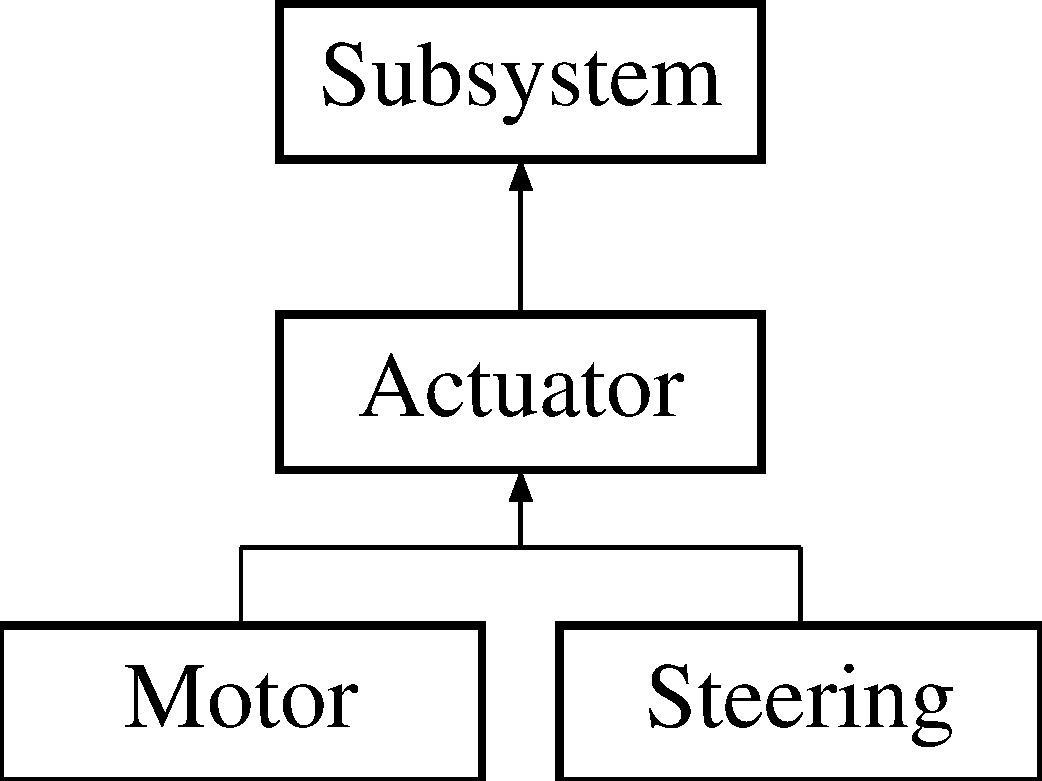
\includegraphics[height=3.000000cm]{classActuator}
\end{center}
\end{figure}
\subsection*{Public Member Functions}
\begin{DoxyCompactItemize}
\item 
\hyperlink{classActuator_ad08f81ed90eb01f4654acb47eff38be6}{Actuator} ()
\begin{DoxyCompactList}\small\item\em \hyperlink{classActuator}{Actuator} default constructor. \end{DoxyCompactList}\item 
\hyperlink{classActuator_a3c19e3031076395a918ab72e1acc8a3c}{$\sim$\-Actuator} ()
\begin{DoxyCompactList}\small\item\em \hyperlink{classActuator}{Actuator} destructor. \end{DoxyCompactList}\item 
void \hyperlink{classActuator_a0ab156ee6321eb413171e7a04ae4d1ca}{init} ()
\begin{DoxyCompactList}\small\item\em initializes the actuator \end{DoxyCompactList}\item 
void \hyperlink{classActuator_abd625b1dfd7dd296e814751e821eae4b}{shutdown} ()
\begin{DoxyCompactList}\small\item\em \hyperlink{classActuator}{Actuator} Shutdown. \end{DoxyCompactList}\item 
virtual void \hyperlink{classActuator_a13e33ed9c5e19a52bc6d0b7e3c0dd2d7}{init\-\_\-device} ()=0
\begin{DoxyCompactList}\small\item\em Virtual function to initialize the actuator device. \end{DoxyCompactList}\item 
virtual void $\ast$ \hyperlink{classActuator_a65fe83ffd7895f3ab028b87a62b3af1d}{read\-\_\-data} (int command)=0
\begin{DoxyCompactList}\small\item\em Reads in data from message to the actuator. \end{DoxyCompactList}\item 
virtual void \hyperlink{classActuator_a05dd923b5162ebad197fc04d07d9771f}{mech\-\_\-control} ()=0
\begin{DoxyCompactList}\small\item\em the mechanical controller function for the actuator. \end{DoxyCompactList}\item 
virtual void \hyperlink{classActuator_ad9c31f9e7f06684835ae526f29d7a096}{mech\-\_\-command} (char $\ast$value)=0
\begin{DoxyCompactList}\small\item\em The mechanical command function issues commands directly to hardware. \end{DoxyCompactList}\item 
virtual void \hyperlink{classActuator_a733c6782030e224bcef26161c77a4d96}{handle\-\_\-message} (\hyperlink{SUBSYS__COMMANDS_8h_ad814416fc1a8c675bea2687d96088a8f}{M\-E\-S\-S\-A\-G\-E} $\ast$message)=0
\begin{DoxyCompactList}\small\item\em Handles message sent to the subsystem. \end{DoxyCompactList}\end{DoxyCompactItemize}
\subsection*{Protected Attributes}
\begin{DoxyCompactItemize}
\item 
pthread\-\_\-t \hyperlink{classActuator_a0097e8667426ce3300ad60bdb6cd9d81}{tmech\-\_\-control}
\end{DoxyCompactItemize}
\subsection*{Additional Inherited Members}


\subsection{Detailed Description}
\hyperlink{classActuator}{Actuator} class manages actuator tasks. 

Sets up collector and analysis tasks on init and cancels tasks on shutdown 

\subsection{Constructor \& Destructor Documentation}
\hypertarget{classActuator_ad08f81ed90eb01f4654acb47eff38be6}{\index{Actuator@{Actuator}!Actuator@{Actuator}}
\index{Actuator@{Actuator}!Actuator@{Actuator}}
\subsubsection[{Actuator}]{\setlength{\rightskip}{0pt plus 5cm}Actuator\-::\-Actuator (
\begin{DoxyParamCaption}
{}
\end{DoxyParamCaption}
)\hspace{0.3cm}{\ttfamily [inline]}}}\label{classActuator_ad08f81ed90eb01f4654acb47eff38be6}


\hyperlink{classActuator}{Actuator} default constructor. 

Sets up subsystem and system message queues and receiver task \hypertarget{classActuator_a3c19e3031076395a918ab72e1acc8a3c}{\index{Actuator@{Actuator}!$\sim$\-Actuator@{$\sim$\-Actuator}}
\index{$\sim$\-Actuator@{$\sim$\-Actuator}!Actuator@{Actuator}}
\subsubsection[{$\sim$\-Actuator}]{\setlength{\rightskip}{0pt plus 5cm}Actuator\-::$\sim$\-Actuator (
\begin{DoxyParamCaption}
{}
\end{DoxyParamCaption}
)}}\label{classActuator_a3c19e3031076395a918ab72e1acc8a3c}


\hyperlink{classActuator}{Actuator} destructor. 

shuts down the actuator subsystem. Calls shutdown. 

\subsection{Member Function Documentation}
\hypertarget{classActuator_a733c6782030e224bcef26161c77a4d96}{\index{Actuator@{Actuator}!handle\-\_\-message@{handle\-\_\-message}}
\index{handle\-\_\-message@{handle\-\_\-message}!Actuator@{Actuator}}
\subsubsection[{handle\-\_\-message}]{\setlength{\rightskip}{0pt plus 5cm}virtual void Actuator\-::handle\-\_\-message (
\begin{DoxyParamCaption}
\item[{{\bf M\-E\-S\-S\-A\-G\-E} $\ast$}]{message}
\end{DoxyParamCaption}
)\hspace{0.3cm}{\ttfamily [pure virtual]}}}\label{classActuator_a733c6782030e224bcef26161c77a4d96}


Handles message sent to the subsystem. 

Virtual function defined at the specific subsystem level. Will handle the messages sent to the actuator from the system controller. Messages could be from command line interface or from another subsystem. 

Implements \hyperlink{classSubsystem_a6205bccfd4906044065d25d8ab1a7bfb}{Subsystem}.



Implemented in \hyperlink{classMotor_add07c258d9b239633a3882a07dc9e4de}{Motor}, and \hyperlink{classSteering_a29e46d1b87ecda7807452ad67005efe1}{Steering}.

\hypertarget{classActuator_a0ab156ee6321eb413171e7a04ae4d1ca}{\index{Actuator@{Actuator}!init@{init}}
\index{init@{init}!Actuator@{Actuator}}
\subsubsection[{init}]{\setlength{\rightskip}{0pt plus 5cm}void Actuator\-::init (
\begin{DoxyParamCaption}
{}
\end{DoxyParamCaption}
)\hspace{0.3cm}{\ttfamily [virtual]}}}\label{classActuator_a0ab156ee6321eb413171e7a04ae4d1ca}


initializes the actuator 

calls the virtual init\-\_\-device function and creates the mechanical control task. 

Implements \hyperlink{classSubsystem_a77a984e8a06bfebb924a6e7ba4f98363}{Subsystem}.

\hypertarget{classActuator_a13e33ed9c5e19a52bc6d0b7e3c0dd2d7}{\index{Actuator@{Actuator}!init\-\_\-device@{init\-\_\-device}}
\index{init\-\_\-device@{init\-\_\-device}!Actuator@{Actuator}}
\subsubsection[{init\-\_\-device}]{\setlength{\rightskip}{0pt plus 5cm}virtual void Actuator\-::init\-\_\-device (
\begin{DoxyParamCaption}
{}
\end{DoxyParamCaption}
)\hspace{0.3cm}{\ttfamily [pure virtual]}}}\label{classActuator_a13e33ed9c5e19a52bc6d0b7e3c0dd2d7}


Virtual function to initialize the actuator device. 

Defined for each actuator, the init\-\_\-device function is responsible for setting the actuator up for control by the mechanical control task. For example in the case of the motor subsystem, the init\-\_\-device task will set up the P\-W\-M, initialize the system variables, and perform other tasks necessary before the motor can be controlled. 

Implemented in \hyperlink{classMotor_a861cd4da09dd25fc02d711a34f25a988}{Motor}, and \hyperlink{classSteering_a57a8011d7d5a4ca608b1b140e21233cb}{Steering}.

\hypertarget{classActuator_ad9c31f9e7f06684835ae526f29d7a096}{\index{Actuator@{Actuator}!mech\-\_\-command@{mech\-\_\-command}}
\index{mech\-\_\-command@{mech\-\_\-command}!Actuator@{Actuator}}
\subsubsection[{mech\-\_\-command}]{\setlength{\rightskip}{0pt plus 5cm}virtual void Actuator\-::mech\-\_\-command (
\begin{DoxyParamCaption}
\item[{char $\ast$}]{value}
\end{DoxyParamCaption}
)\hspace{0.3cm}{\ttfamily [pure virtual]}}}\label{classActuator_ad9c31f9e7f06684835ae526f29d7a096}


The mechanical command function issues commands directly to hardware. 

The mechanical command function is typically called from the mech\-\_\-control function and will issue the actual commands to hardware necessary to control the actuator. For example, for the motor subsystem, this function will write to P\-W\-M. 

Implemented in \hyperlink{classMotor_a3edca1dcb0f3df55eccc09ffb14426a4}{Motor}, and \hyperlink{classSteering_a0ae09490e872d21d211ddfdc446d14d1}{Steering}.

\hypertarget{classActuator_a05dd923b5162ebad197fc04d07d9771f}{\index{Actuator@{Actuator}!mech\-\_\-control@{mech\-\_\-control}}
\index{mech\-\_\-control@{mech\-\_\-control}!Actuator@{Actuator}}
\subsubsection[{mech\-\_\-control}]{\setlength{\rightskip}{0pt plus 5cm}virtual void Actuator\-::mech\-\_\-control (
\begin{DoxyParamCaption}
{}
\end{DoxyParamCaption}
)\hspace{0.3cm}{\ttfamily [pure virtual]}}}\label{classActuator_a05dd923b5162ebad197fc04d07d9771f}


the mechanical controller function for the actuator. 

Run in the mech\-\_\-control thread and waits for a sync semaphore before issuing a mechanical command if the subsystem is enabled. 

Implemented in \hyperlink{classMotor_a9902b2c030a06ca8a4e2f10c3530dbec}{Motor}, and \hyperlink{classSteering_a5b7b0a053607ad891b7d2826093da6ac}{Steering}.

\hypertarget{classActuator_a65fe83ffd7895f3ab028b87a62b3af1d}{\index{Actuator@{Actuator}!read\-\_\-data@{read\-\_\-data}}
\index{read\-\_\-data@{read\-\_\-data}!Actuator@{Actuator}}
\subsubsection[{read\-\_\-data}]{\setlength{\rightskip}{0pt plus 5cm}virtual void$\ast$ Actuator\-::read\-\_\-data (
\begin{DoxyParamCaption}
\item[{int}]{command}
\end{DoxyParamCaption}
)\hspace{0.3cm}{\ttfamily [pure virtual]}}}\label{classActuator_a65fe83ffd7895f3ab028b87a62b3af1d}


Reads in data from message to the actuator. 

Will read data into appropriate data type and then cast to a void$\ast$ and return. The type of data received depends on the message command. For example if trying to set the motor pwm duty cycle, a three byte char$\ast$ is expected. This function will read the data in from standard in (using cin) into an appropriate datatype for the given command and will return the data to the system message handler for further processing. 

Implements \hyperlink{classSubsystem_a85307df3e46421814204f77929e893aa}{Subsystem}.



Implemented in \hyperlink{classMotor_a1727e2d2dfd483c9c85824915a6aeeb8}{Motor}, and \hyperlink{classSteering_afda4f2951e5be114abf988a8e5943a96}{Steering}.

\hypertarget{classActuator_abd625b1dfd7dd296e814751e821eae4b}{\index{Actuator@{Actuator}!shutdown@{shutdown}}
\index{shutdown@{shutdown}!Actuator@{Actuator}}
\subsubsection[{shutdown}]{\setlength{\rightskip}{0pt plus 5cm}void Actuator\-::shutdown (
\begin{DoxyParamCaption}
{}
\end{DoxyParamCaption}
)\hspace{0.3cm}{\ttfamily [virtual]}}}\label{classActuator_abd625b1dfd7dd296e814751e821eae4b}


\hyperlink{classActuator}{Actuator} Shutdown. 

shuts down the actuator subsystem. Cancels the mechanical control thread. 

Implements \hyperlink{classSubsystem_a510e18f972a3d86d7a47432dafa1ce4c}{Subsystem}.



\subsection{Member Data Documentation}
\hypertarget{classActuator_a0097e8667426ce3300ad60bdb6cd9d81}{\index{Actuator@{Actuator}!tmech\-\_\-control@{tmech\-\_\-control}}
\index{tmech\-\_\-control@{tmech\-\_\-control}!Actuator@{Actuator}}
\subsubsection[{tmech\-\_\-control}]{\setlength{\rightskip}{0pt plus 5cm}pthread\-\_\-t Actuator\-::tmech\-\_\-control\hspace{0.3cm}{\ttfamily [protected]}}}\label{classActuator_a0097e8667426ce3300ad60bdb6cd9d81}
the mech\-\_\-control thread 

The documentation for this class was generated from the following files\-:\begin{DoxyCompactItemize}
\item 
/home/keith/realtime/Actuator.\-h\item 
/home/keith/realtime/Actuator.\-cpp\end{DoxyCompactItemize}

\input{classADC}
\hypertarget{classCompass}{\section{Compass Class Reference}
\label{classCompass}\index{Compass@{Compass}}
}


compass data collection and analysis  




{\ttfamily \#include $<$Compass.\-h$>$}

Inheritance diagram for Compass\-:\begin{figure}[H]
\begin{center}
\leavevmode
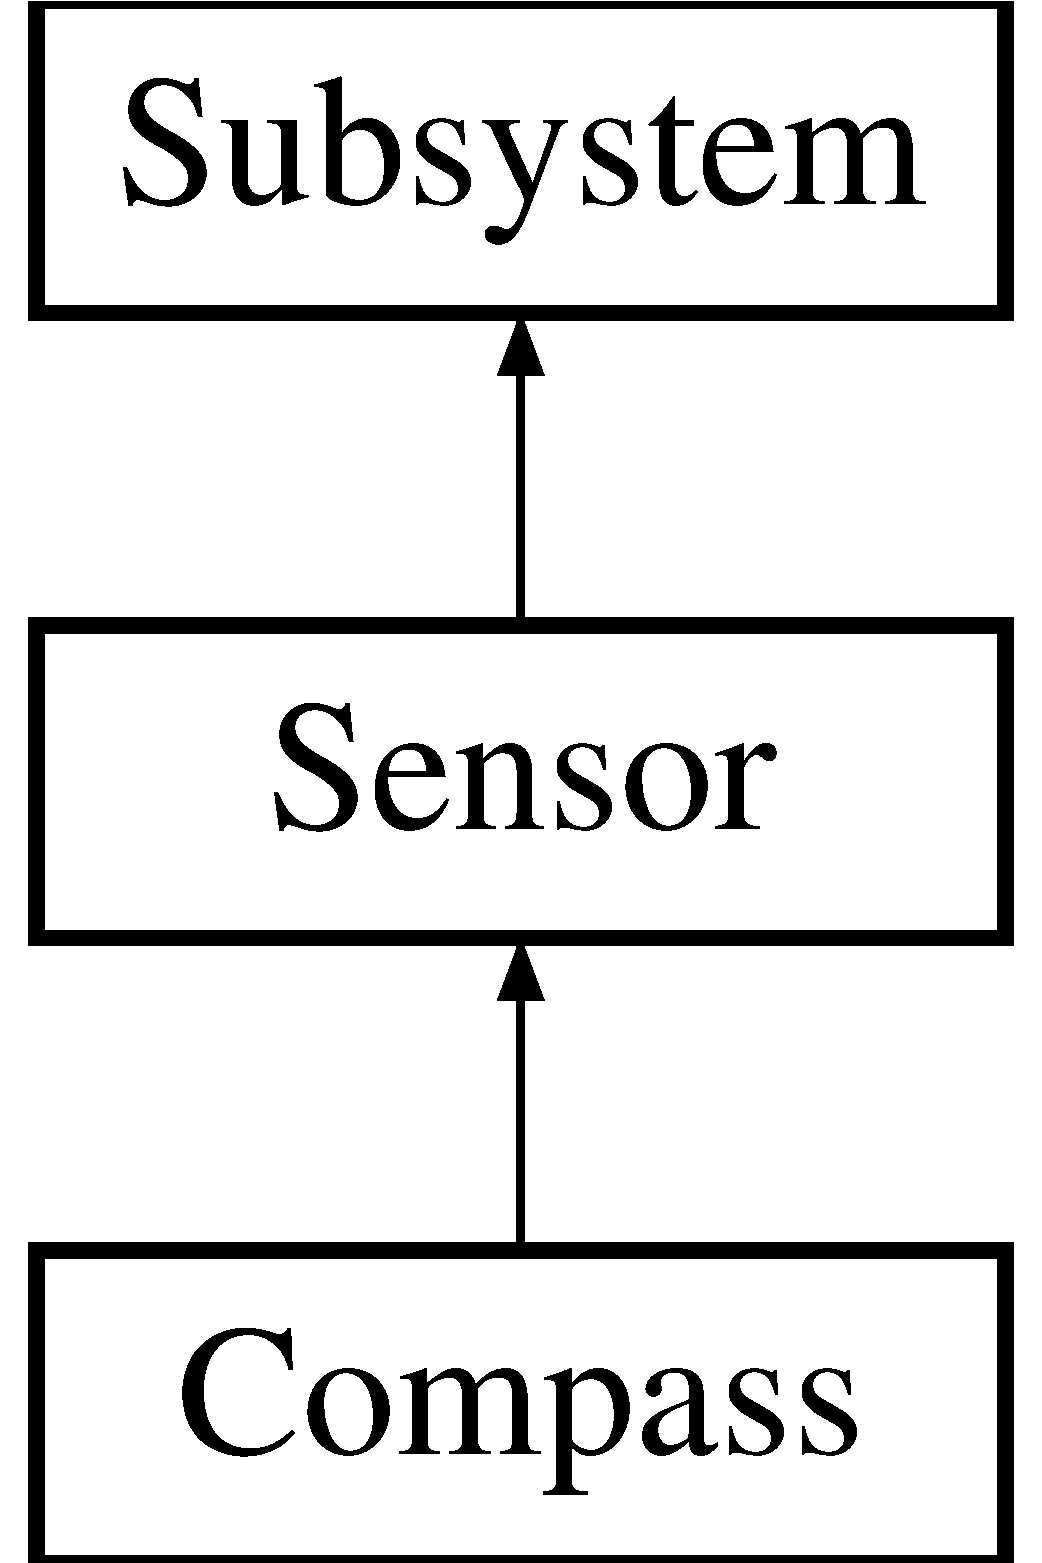
\includegraphics[height=3.000000cm]{classCompass}
\end{center}
\end{figure}
\subsection*{Public Member Functions}
\begin{DoxyCompactItemize}
\item 
\hyperlink{classCompass_a68bd2a073cc0d461b2b46529aae04765}{Compass} ()
\begin{DoxyCompactList}\small\item\em \hyperlink{classCompass}{Compass} default constructor. \end{DoxyCompactList}\item 
float \hyperlink{classCompass_aa4132c05a4e20e95633c72776385bc42}{data\-\_\-grab} ()
\begin{DoxyCompactList}\small\item\em grabs data from compass \end{DoxyCompactList}\item 
void \hyperlink{classCompass_a5cc2b71700af542b5aafadea4820a476}{init\-\_\-sensor} ()
\begin{DoxyCompactList}\small\item\em Initializes the \hyperlink{classCompass}{Compass}. \end{DoxyCompactList}\item 
void \hyperlink{classCompass_ae8d7f3417a27b1d18487b96ca07dd32b}{collector} ()
\begin{DoxyCompactList}\small\item\em collects data from the \hyperlink{classCompass}{Compass} \end{DoxyCompactList}\item 
void \hyperlink{classCompass_a4dd6402d0ece9203c6b92670265b4c8d}{analysis} ()
\begin{DoxyCompactList}\small\item\em Performs the analysis of the data collected from the compass and commands the actuators. \end{DoxyCompactList}\item 
void \hyperlink{classCompass_a1fb0f64b335e8f1d4f27dc2067312b4a}{handle\-\_\-message} (\hyperlink{SUBSYS__COMMANDS_8h_ad814416fc1a8c675bea2687d96088a8f}{M\-E\-S\-S\-A\-G\-E} $\ast$message)
\begin{DoxyCompactList}\small\item\em Handles messages sent to the compass subsystem. \end{DoxyCompactList}\item 
void $\ast$ \hyperlink{classCompass_ab55d084e2d643df0a1970f5868d0c5a8}{read\-\_\-data} (int command)
\begin{DoxyCompactList}\small\item\em Reads in data from message to the compass. \end{DoxyCompactList}\end{DoxyCompactItemize}
\subsection*{Public Attributes}
\begin{DoxyCompactItemize}
\item 
\hyperlink{SUBSYS__COMMANDS_8h_ad814416fc1a8c675bea2687d96088a8f}{M\-E\-S\-S\-A\-G\-E} \hyperlink{classCompass_a15cd7eda15b824c8d5821a46667b861c}{hard\-\_\-right}
\item 
\hyperlink{SUBSYS__COMMANDS_8h_ad814416fc1a8c675bea2687d96088a8f}{M\-E\-S\-S\-A\-G\-E} \hyperlink{classCompass_a9e9ff6610d60e6fd915984a3f3e40e13}{slight\-\_\-right}
\item 
\hyperlink{SUBSYS__COMMANDS_8h_ad814416fc1a8c675bea2687d96088a8f}{M\-E\-S\-S\-A\-G\-E} \hyperlink{classCompass_aa11186aa6caf9dced42940552bf24da2}{straight}
\item 
\hyperlink{SUBSYS__COMMANDS_8h_ad814416fc1a8c675bea2687d96088a8f}{M\-E\-S\-S\-A\-G\-E} \hyperlink{classCompass_a5cbc2cebdd91222c5ccf5bd28aa35ced}{hard\-\_\-left}
\item 
\hyperlink{SUBSYS__COMMANDS_8h_ad814416fc1a8c675bea2687d96088a8f}{M\-E\-S\-S\-A\-G\-E} \hyperlink{classCompass_a9e0a282c1253451fd7967646074102ee}{slight\-\_\-left}
\end{DoxyCompactItemize}
\subsection*{Protected Attributes}
\begin{DoxyCompactItemize}
\item 
float \hyperlink{classCompass_ac888a4dacdc477e53c99fe8e110966ae}{desired\-\_\-heading}
\item 
float \hyperlink{classCompass_af0f87a131e2c9833f7d52bed1a39bf75}{meas\-\_\-heading}
\item 
sem\-\_\-t \hyperlink{classCompass_ace6e13b91461366609f093fef09188d9}{collect\-\_\-analysis\-\_\-sync}
\item 
int \hyperlink{classCompass_a44b0e4223918e3b139e54d54a0e3daad}{compass\-\_\-fd}
\item 
char \hyperlink{classCompass_a6ff33d93efe79539c75dbee45efdc97c}{compass\-\_\-filepath} \mbox{[}40\mbox{]}
\end{DoxyCompactItemize}


\subsection{Detailed Description}
compass data collection and analysis 

Collects data from the compass and analyzes the data. Sends system messages to control actuators 

\subsection{Constructor \& Destructor Documentation}
\hypertarget{classCompass_a68bd2a073cc0d461b2b46529aae04765}{\index{Compass@{Compass}!Compass@{Compass}}
\index{Compass@{Compass}!Compass@{Compass}}
\subsubsection[{Compass}]{\setlength{\rightskip}{0pt plus 5cm}Compass\-::\-Compass (
\begin{DoxyParamCaption}
{}
\end{DoxyParamCaption}
)}}\label{classCompass_a68bd2a073cc0d461b2b46529aae04765}


\hyperlink{classCompass}{Compass} default constructor. 

Sets subsystem parameters and sets up the collect/analysis task sync semaphore. 

\subsection{Member Function Documentation}
\hypertarget{classCompass_a4dd6402d0ece9203c6b92670265b4c8d}{\index{Compass@{Compass}!analysis@{analysis}}
\index{analysis@{analysis}!Compass@{Compass}}
\subsubsection[{analysis}]{\setlength{\rightskip}{0pt plus 5cm}void Compass\-::analysis (
\begin{DoxyParamCaption}
{}
\end{DoxyParamCaption}
)\hspace{0.3cm}{\ttfamily [virtual]}}}\label{classCompass_a4dd6402d0ece9203c6b92670265b4c8d}


Performs the analysis of the data collected from the compass and commands the actuators. 

The analysis function executes in the analysis thread and is synced with the collector task by the collect\-\_\-analysis\-\_\-sync semaphore. Depending on the difference between the current and desired headings, messages will be sent to the \hyperlink{classSteering}{Steering} subsystem using the system message queue to change course. 

Implements \hyperlink{classSensor_a595d8d9cd87dd3704fad2a313c709a7e}{Sensor}.

\hypertarget{classCompass_ae8d7f3417a27b1d18487b96ca07dd32b}{\index{Compass@{Compass}!collector@{collector}}
\index{collector@{collector}!Compass@{Compass}}
\subsubsection[{collector}]{\setlength{\rightskip}{0pt plus 5cm}void Compass\-::collector (
\begin{DoxyParamCaption}
{}
\end{DoxyParamCaption}
)\hspace{0.3cm}{\ttfamily [virtual]}}}\label{classCompass_ae8d7f3417a27b1d18487b96ca07dd32b}


collects data from the \hyperlink{classCompass}{Compass} 

The collector function executes in the collector thread and executes indefinitely at a frequency of 20\-Hz. It calls the data\-\_\-grab to do the actual communication with the hardware to provide a layer of abstraction between the software and specifics of the hardware. It can optionally average data prior to analysis if the system is expected to be under heavy load and the tasks are not schedulable with the typical release frequencies (averaging will have the effect that the analysis task will be released less frequently). 

Implements \hyperlink{classSensor_ae4ec41b880d44feb898da5c62c3203c9}{Sensor}.

\hypertarget{classCompass_aa4132c05a4e20e95633c72776385bc42}{\index{Compass@{Compass}!data\-\_\-grab@{data\-\_\-grab}}
\index{data\-\_\-grab@{data\-\_\-grab}!Compass@{Compass}}
\subsubsection[{data\-\_\-grab}]{\setlength{\rightskip}{0pt plus 5cm}float Compass\-::data\-\_\-grab (
\begin{DoxyParamCaption}
{}
\end{DoxyParamCaption}
)}}\label{classCompass_aa4132c05a4e20e95633c72776385bc42}


grabs data from compass 

Gets data from the compass over I2\-C. Returns the current heading in degrees as a float. \hypertarget{classCompass_a1fb0f64b335e8f1d4f27dc2067312b4a}{\index{Compass@{Compass}!handle\-\_\-message@{handle\-\_\-message}}
\index{handle\-\_\-message@{handle\-\_\-message}!Compass@{Compass}}
\subsubsection[{handle\-\_\-message}]{\setlength{\rightskip}{0pt plus 5cm}void Compass\-::handle\-\_\-message (
\begin{DoxyParamCaption}
\item[{{\bf M\-E\-S\-S\-A\-G\-E} $\ast$}]{message}
\end{DoxyParamCaption}
)\hspace{0.3cm}{\ttfamily [virtual]}}}\label{classCompass_a1fb0f64b335e8f1d4f27dc2067312b4a}


Handles messages sent to the compass subsystem. 

Performs tasks determined by the command part of the message. For example the command C\-P\-S\-\_\-\-S\-E\-T\-\_\-\-H\-E\-A\-D\-I\-N\-G is used to set the desired heading. Messages could be from command line interface or from another subsystem. 

Implements \hyperlink{classSensor_a45533b253f81f85d1b6fcea902a5692b}{Sensor}.

\hypertarget{classCompass_a5cc2b71700af542b5aafadea4820a476}{\index{Compass@{Compass}!init\-\_\-sensor@{init\-\_\-sensor}}
\index{init\-\_\-sensor@{init\-\_\-sensor}!Compass@{Compass}}
\subsubsection[{init\-\_\-sensor}]{\setlength{\rightskip}{0pt plus 5cm}void Compass\-::init\-\_\-sensor (
\begin{DoxyParamCaption}
{}
\end{DoxyParamCaption}
)\hspace{0.3cm}{\ttfamily [virtual]}}}\label{classCompass_a5cc2b71700af542b5aafadea4820a476}


Initializes the \hyperlink{classCompass}{Compass}. 

Sets up the I2\-C driver and sets up the compass hardware to continuously spit out data at 20\-Hz. 

Implements \hyperlink{classSensor_a11b28f6bc91d6f69e734e13ab0e64f56}{Sensor}.

\hypertarget{classCompass_ab55d084e2d643df0a1970f5868d0c5a8}{\index{Compass@{Compass}!read\-\_\-data@{read\-\_\-data}}
\index{read\-\_\-data@{read\-\_\-data}!Compass@{Compass}}
\subsubsection[{read\-\_\-data}]{\setlength{\rightskip}{0pt plus 5cm}void $\ast$ Compass\-::read\-\_\-data (
\begin{DoxyParamCaption}
\item[{int}]{command}
\end{DoxyParamCaption}
)\hspace{0.3cm}{\ttfamily [virtual]}}}\label{classCompass_ab55d084e2d643df0a1970f5868d0c5a8}


Reads in data from message to the compass. 

Will read data into appropriate data type and then cast to a void$\ast$ and return. The type of data received depends on the message command. For example if trying to set the desired heading, a float is expected. This function will read the data in from standard in (using cin) into an appropriate datatype for the given command and will return the data to the system message handler for further processing. 

Implements \hyperlink{classSensor_acf4ff5c6c8f793ed47a8105b94ff7c3e}{Sensor}.



\subsection{Member Data Documentation}
\hypertarget{classCompass_ace6e13b91461366609f093fef09188d9}{\index{Compass@{Compass}!collect\-\_\-analysis\-\_\-sync@{collect\-\_\-analysis\-\_\-sync}}
\index{collect\-\_\-analysis\-\_\-sync@{collect\-\_\-analysis\-\_\-sync}!Compass@{Compass}}
\subsubsection[{collect\-\_\-analysis\-\_\-sync}]{\setlength{\rightskip}{0pt plus 5cm}sem\-\_\-t Compass\-::collect\-\_\-analysis\-\_\-sync\hspace{0.3cm}{\ttfamily [protected]}}}\label{classCompass_ace6e13b91461366609f093fef09188d9}
The collect/analysis sync semaphore \hypertarget{classCompass_a44b0e4223918e3b139e54d54a0e3daad}{\index{Compass@{Compass}!compass\-\_\-fd@{compass\-\_\-fd}}
\index{compass\-\_\-fd@{compass\-\_\-fd}!Compass@{Compass}}
\subsubsection[{compass\-\_\-fd}]{\setlength{\rightskip}{0pt plus 5cm}int Compass\-::compass\-\_\-fd\hspace{0.3cm}{\ttfamily [protected]}}}\label{classCompass_a44b0e4223918e3b139e54d54a0e3daad}
The i2c file descriptor for the compass \hypertarget{classCompass_a6ff33d93efe79539c75dbee45efdc97c}{\index{Compass@{Compass}!compass\-\_\-filepath@{compass\-\_\-filepath}}
\index{compass\-\_\-filepath@{compass\-\_\-filepath}!Compass@{Compass}}
\subsubsection[{compass\-\_\-filepath}]{\setlength{\rightskip}{0pt plus 5cm}char Compass\-::compass\-\_\-filepath\mbox{[}40\mbox{]}\hspace{0.3cm}{\ttfamily [protected]}}}\label{classCompass_a6ff33d93efe79539c75dbee45efdc97c}
The filename for the compass device. (will be a device in /dev). \hypertarget{classCompass_ac888a4dacdc477e53c99fe8e110966ae}{\index{Compass@{Compass}!desired\-\_\-heading@{desired\-\_\-heading}}
\index{desired\-\_\-heading@{desired\-\_\-heading}!Compass@{Compass}}
\subsubsection[{desired\-\_\-heading}]{\setlength{\rightskip}{0pt plus 5cm}float Compass\-::desired\-\_\-heading\hspace{0.3cm}{\ttfamily [protected]}}}\label{classCompass_ac888a4dacdc477e53c99fe8e110966ae}
The desired heading \hypertarget{classCompass_a5cbc2cebdd91222c5ccf5bd28aa35ced}{\index{Compass@{Compass}!hard\-\_\-left@{hard\-\_\-left}}
\index{hard\-\_\-left@{hard\-\_\-left}!Compass@{Compass}}
\subsubsection[{hard\-\_\-left}]{\setlength{\rightskip}{0pt plus 5cm}{\bf M\-E\-S\-S\-A\-G\-E} Compass\-::hard\-\_\-left}}\label{classCompass_a5cbc2cebdd91222c5ccf5bd28aa35ced}
A message that will, when sent, issue a command to the \hyperlink{classSteering}{Steering} subsystem to turn hard left \hypertarget{classCompass_a15cd7eda15b824c8d5821a46667b861c}{\index{Compass@{Compass}!hard\-\_\-right@{hard\-\_\-right}}
\index{hard\-\_\-right@{hard\-\_\-right}!Compass@{Compass}}
\subsubsection[{hard\-\_\-right}]{\setlength{\rightskip}{0pt plus 5cm}{\bf M\-E\-S\-S\-A\-G\-E} Compass\-::hard\-\_\-right}}\label{classCompass_a15cd7eda15b824c8d5821a46667b861c}
A message that will, when sent, issue a command to the \hyperlink{classSteering}{Steering} subsystem to turn hard right \hypertarget{classCompass_af0f87a131e2c9833f7d52bed1a39bf75}{\index{Compass@{Compass}!meas\-\_\-heading@{meas\-\_\-heading}}
\index{meas\-\_\-heading@{meas\-\_\-heading}!Compass@{Compass}}
\subsubsection[{meas\-\_\-heading}]{\setlength{\rightskip}{0pt plus 5cm}float Compass\-::meas\-\_\-heading\hspace{0.3cm}{\ttfamily [protected]}}}\label{classCompass_af0f87a131e2c9833f7d52bed1a39bf75}
The last measured heading. Updated at 20\-Hz. \hypertarget{classCompass_a9e0a282c1253451fd7967646074102ee}{\index{Compass@{Compass}!slight\-\_\-left@{slight\-\_\-left}}
\index{slight\-\_\-left@{slight\-\_\-left}!Compass@{Compass}}
\subsubsection[{slight\-\_\-left}]{\setlength{\rightskip}{0pt plus 5cm}{\bf M\-E\-S\-S\-A\-G\-E} Compass\-::slight\-\_\-left}}\label{classCompass_a9e0a282c1253451fd7967646074102ee}
A message that will, when sent, issue a command to the \hyperlink{classSteering}{Steering} subsystem to turn slightly left \hypertarget{classCompass_a9e9ff6610d60e6fd915984a3f3e40e13}{\index{Compass@{Compass}!slight\-\_\-right@{slight\-\_\-right}}
\index{slight\-\_\-right@{slight\-\_\-right}!Compass@{Compass}}
\subsubsection[{slight\-\_\-right}]{\setlength{\rightskip}{0pt plus 5cm}{\bf M\-E\-S\-S\-A\-G\-E} Compass\-::slight\-\_\-right}}\label{classCompass_a9e9ff6610d60e6fd915984a3f3e40e13}
A message that will, when sent, issue a command to the \hyperlink{classSteering}{Steering} subsystem to turn slightly right \hypertarget{classCompass_aa11186aa6caf9dced42940552bf24da2}{\index{Compass@{Compass}!straight@{straight}}
\index{straight@{straight}!Compass@{Compass}}
\subsubsection[{straight}]{\setlength{\rightskip}{0pt plus 5cm}{\bf M\-E\-S\-S\-A\-G\-E} Compass\-::straight}}\label{classCompass_aa11186aa6caf9dced42940552bf24da2}
A message that will, when sent, issue a command to the \hyperlink{classSteering}{Steering} subsystem to go straight 

The documentation for this class was generated from the following files\-:\begin{DoxyCompactItemize}
\item 
/home/keith/realtime/Compass.\-h\item 
/home/keith/realtime/Compass.\-cpp\end{DoxyCompactItemize}

\hypertarget{classGPS}{\section{G\-P\-S Class Reference}
\label{classGPS}\index{G\-P\-S@{G\-P\-S}}
}


\hyperlink{classGPS}{G\-P\-S} data collection and analysis.  




{\ttfamily \#include $<$G\-P\-S.\-h$>$}

Inheritance diagram for G\-P\-S\-:\begin{figure}[H]
\begin{center}
\leavevmode
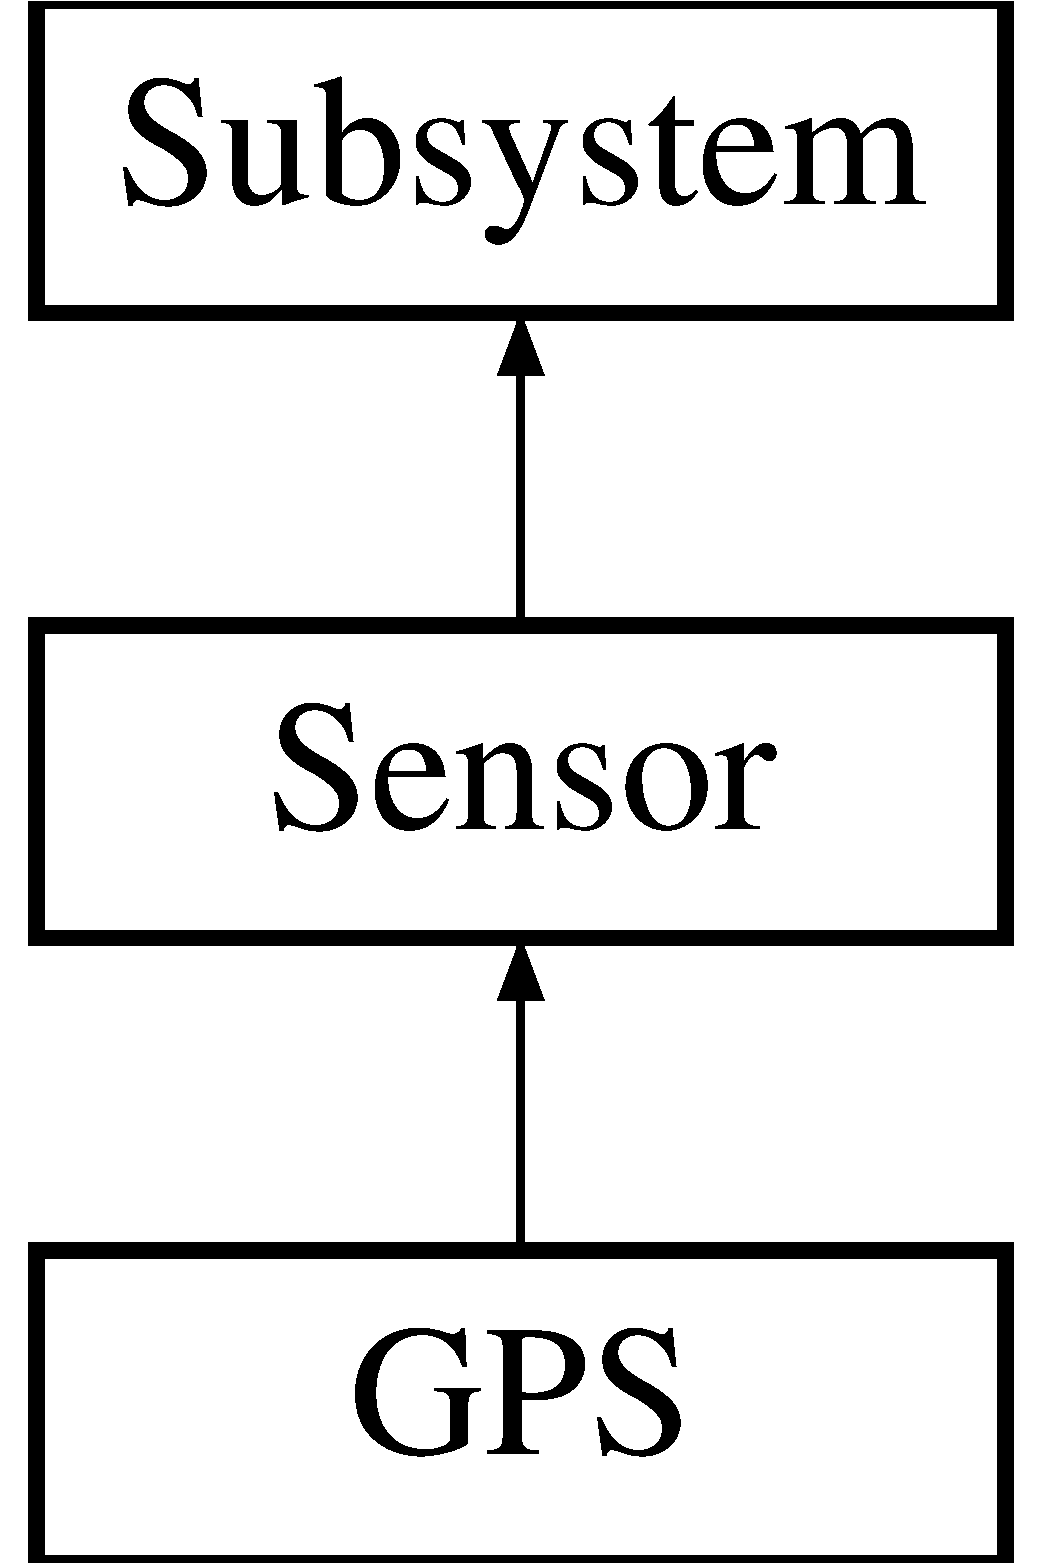
\includegraphics[height=3.000000cm]{classGPS}
\end{center}
\end{figure}
\subsection*{Classes}
\begin{DoxyCompactItemize}
\item 
class \hyperlink{classGPS_1_1GPSWayPoint}{G\-P\-S\-Way\-Point}
\begin{DoxyCompactList}\small\item\em Stores \hyperlink{classGPS}{G\-P\-S} Way\-Points as a linked list. \end{DoxyCompactList}\item 
class \hyperlink{classGPS_1_1LatLon}{Lat\-Lon}
\begin{DoxyCompactList}\small\item\em Structure that hold latitude and longitude. \end{DoxyCompactList}\end{DoxyCompactItemize}
\subsection*{Public Member Functions}
\begin{DoxyCompactItemize}
\item 
\hyperlink{classGPS_a0c347a188512d0d5cf7ed5c91b145fc4}{G\-P\-S} ()
\begin{DoxyCompactList}\small\item\em \hyperlink{classGPS}{G\-P\-S} default constructor. \end{DoxyCompactList}\item 
\hypertarget{classGPS_afe84b00ea93254fcb8b84a0f2b240c9d}{\hyperlink{classGPS_afe84b00ea93254fcb8b84a0f2b240c9d}{$\sim$\-G\-P\-S} ()}\label{classGPS_afe84b00ea93254fcb8b84a0f2b240c9d}

\begin{DoxyCompactList}\small\item\em deconstructor \end{DoxyCompactList}\item 
void \hyperlink{classGPS_acd4e4d75709b2b897972f4ff89a2bdab}{data\-\_\-grab} (\hyperlink{classGPS_1_1LatLon}{Lat\-Lon} \&output)
\begin{DoxyCompactList}\small\item\em grabs data from \hyperlink{classGPS}{G\-P\-S} \end{DoxyCompactList}\item 
\hypertarget{classGPS_aebb999362899800a7e372e873bb5b943}{void \hyperlink{classGPS_aebb999362899800a7e372e873bb5b943}{init\-\_\-sensor} ()}\label{classGPS_aebb999362899800a7e372e873bb5b943}

\begin{DoxyCompactList}\small\item\em initialize the \hyperlink{classGPS}{G\-P\-S} connection \end{DoxyCompactList}\item 
void \hyperlink{classGPS_a17383568c4ed86a0adfdd5c88b6591d4}{collector} ()
\begin{DoxyCompactList}\small\item\em collects \hyperlink{classGPS}{G\-P\-S} data \end{DoxyCompactList}\item 
void \hyperlink{classGPS_a4dca50736c5e49f831515219536823b2}{analysis} ()
\begin{DoxyCompactList}\small\item\em data analysis \end{DoxyCompactList}\item 
void $\ast$ \hyperlink{classGPS_aa04076536ee9f7e2679895c69b07ad58}{read\-\_\-data} (int command)
\item 
\hypertarget{classGPS_a803a498352e30044136502a9e036d380}{void \hyperlink{classGPS_a803a498352e30044136502a9e036d380}{handle\-\_\-message} (\hyperlink{SUBSYS__COMMANDS_8h_ad814416fc1a8c675bea2687d96088a8f}{M\-E\-S\-S\-A\-G\-E} $\ast$message)}\label{classGPS_a803a498352e30044136502a9e036d380}

\begin{DoxyCompactList}\small\item\em handles messages sent to the \hyperlink{classGPS}{G\-P\-S} subsystem \end{DoxyCompactList}\item 
\hypertarget{classGPS_abb0d819282c6575d1c9dfadce5270238}{bool \hyperlink{classGPS_abb0d819282c6575d1c9dfadce5270238}{convert\-\_\-data} (char $\ast$input, int length, \hyperlink{classGPS_1_1LatLon}{Lat\-Lon} \&output)}\label{classGPS_abb0d819282c6575d1c9dfadce5270238}

\begin{DoxyCompactList}\small\item\em Converts the input command into lat/long and stores in output. \end{DoxyCompactList}\item 
\hypertarget{classGPS_ae6fac25305f26521d3cb313608224cbf}{bool \hyperlink{classGPS_ae6fac25305f26521d3cb313608224cbf}{update\-Way\-Point} ()}\label{classGPS_ae6fac25305f26521d3cb313608224cbf}

\begin{DoxyCompactList}\small\item\em Update waypoint if necissary. \end{DoxyCompactList}\item 
\hypertarget{classGPS_a2a02aee137990e44240c60148d4dd892}{bool \hyperlink{classGPS_a2a02aee137990e44240c60148d4dd892}{add\-Way\-Point} (\hyperlink{classGPS_1_1LatLon}{Lat\-Lon} latlon, double radius, int index=-\/1)}\label{classGPS_a2a02aee137990e44240c60148d4dd892}

\begin{DoxyCompactList}\small\item\em Add Waypoint. \end{DoxyCompactList}\item 
\hypertarget{classGPS_a5c2fe388fb6d9f324f9f00e1abdfd5ed}{\hyperlink{classGPS_1_1LatLon}{Lat\-Lon} \hyperlink{classGPS_a5c2fe388fb6d9f324f9f00e1abdfd5ed}{get\-Loc\-Buffer\-Avg} ()}\label{classGPS_a5c2fe388fb6d9f324f9f00e1abdfd5ed}

\begin{DoxyCompactList}\small\item\em Get location from rolling buffer (averaged) \end{DoxyCompactList}\item 
double \hyperlink{classGPS_a142cd2ff428450d1145ddaaa4e2974a8}{get\-Angle} (\hyperlink{classGPS_1_1LatLon}{Lat\-Lon} start\-Loc, \hyperlink{classGPS_1_1LatLon}{Lat\-Lon} eennd\-Loc)
\begin{DoxyCompactList}\small\item\em Get the angle between two lat long. \end{DoxyCompactList}\item 
\hypertarget{classGPS_a988b4a8104bc8e93d1225cad026ce578}{void \hyperlink{classGPS_a988b4a8104bc8e93d1225cad026ce578}{set\-Loc\-Buffer} (const \hyperlink{classGPS_1_1LatLon}{G\-P\-S\-::\-Lat\-Lon} location)}\label{classGPS_a988b4a8104bc8e93d1225cad026ce578}

\begin{DoxyCompactList}\small\item\em Add a value to the lat long rolling buffer. \end{DoxyCompactList}\end{DoxyCompactItemize}
\subsection*{Protected Attributes}
\begin{DoxyCompactItemize}
\item 
int \hyperlink{classGPS_a14c36e0dcc27dfa5e1381b9a4b25c2ce}{output\-\_\-heading}
\item 
int \hyperlink{classGPS_a62ebacee895a13c211bfd372b818b680}{serial\-\_\-port}
\item 
\hyperlink{classGPS_1_1GPSWayPoint}{G\-P\-S\-Way\-Point} $\ast$ \hyperlink{classGPS_a9deda2a96578019d9512a8ec74a93191}{target}
\item 
\hyperlink{classGPS_1_1GPSWayPoint}{G\-P\-S\-Way\-Point} $\ast$ \hyperlink{classGPS_ad1fea42571de73f9b9278cc329490457}{head\-Ptr}
\item 
\hyperlink{classGPS_1_1LatLon}{Lat\-Lon} \hyperlink{classGPS_a78bd0e171c43d44a60349cba2d05f29b}{loc\-Buffer} \mbox{[}G\-P\-S\-\_\-\-R\-O\-L\-L\-B\-U\-F\-F\-\_\-\-S\-I\-Z\-E $\ast$2\mbox{]}
\item 
int \hyperlink{classGPS_a8a593af52417cf88df7c6c7172d7caf7}{loc\-Buffer\-Index}
\item 
int \hyperlink{classGPS_ac85c17369384b4f9ddb0d0358df9d1cf}{loc\-Buffer\-Index\-B}
\item 
sem\-\_\-t \hyperlink{classGPS_ab0d29060e79b34b84fa06847a36de2e7}{collect\-\_\-analysis\-\_\-sync}
\item 
double \hyperlink{classGPS_aa0e370ef448d131c54e3b1d626576cd2}{temp\-\_\-lat}
\item 
double \hyperlink{classGPS_a4b108cba87ab121532c180e214d0c7fa}{temp\-\_\-lon}
\end{DoxyCompactItemize}
\subsection*{Additional Inherited Members}


\subsection{Detailed Description}
\hyperlink{classGPS}{G\-P\-S} data collection and analysis. 

Define this variable to enable printf debugging

Collects data from the \hyperlink{classGPS}{G\-P\-S} and analyzes the data. Sends system messages to control actuators 

\subsection{Constructor \& Destructor Documentation}
\hypertarget{classGPS_a0c347a188512d0d5cf7ed5c91b145fc4}{\index{G\-P\-S@{G\-P\-S}!G\-P\-S@{G\-P\-S}}
\index{G\-P\-S@{G\-P\-S}!GPS@{G\-P\-S}}
\subsubsection[{G\-P\-S}]{\setlength{\rightskip}{0pt plus 5cm}G\-P\-S\-::\-G\-P\-S (
\begin{DoxyParamCaption}
{}
\end{DoxyParamCaption}
)}}\label{classGPS_a0c347a188512d0d5cf7ed5c91b145fc4}


\hyperlink{classGPS}{G\-P\-S} default constructor. 

sets subsystem parameters 

\subsection{Member Function Documentation}
\hypertarget{classGPS_a4dca50736c5e49f831515219536823b2}{\index{G\-P\-S@{G\-P\-S}!analysis@{analysis}}
\index{analysis@{analysis}!GPS@{G\-P\-S}}
\subsubsection[{analysis}]{\setlength{\rightskip}{0pt plus 5cm}void G\-P\-S\-::analysis (
\begin{DoxyParamCaption}
{}
\end{DoxyParamCaption}
)\hspace{0.3cm}{\ttfamily [virtual]}}}\label{classGPS_a4dca50736c5e49f831515219536823b2}


data analysis 

Issues commands to acuators based on \hyperlink{classGPS}{G\-P\-S} data 

Implements \hyperlink{classSensor_a595d8d9cd87dd3704fad2a313c709a7e}{Sensor}.

\hypertarget{classGPS_a17383568c4ed86a0adfdd5c88b6591d4}{\index{G\-P\-S@{G\-P\-S}!collector@{collector}}
\index{collector@{collector}!GPS@{G\-P\-S}}
\subsubsection[{collector}]{\setlength{\rightskip}{0pt plus 5cm}void G\-P\-S\-::collector (
\begin{DoxyParamCaption}
{}
\end{DoxyParamCaption}
)\hspace{0.3cm}{\ttfamily [virtual]}}}\label{classGPS_a17383568c4ed86a0adfdd5c88b6591d4}


collects \hyperlink{classGPS}{G\-P\-S} data 

collects \hyperlink{classGPS}{G\-P\-S} data and averages data prior to analysis 

Implements \hyperlink{classSensor_ae4ec41b880d44feb898da5c62c3203c9}{Sensor}.

\hypertarget{classGPS_acd4e4d75709b2b897972f4ff89a2bdab}{\index{G\-P\-S@{G\-P\-S}!data\-\_\-grab@{data\-\_\-grab}}
\index{data\-\_\-grab@{data\-\_\-grab}!GPS@{G\-P\-S}}
\subsubsection[{data\-\_\-grab}]{\setlength{\rightskip}{0pt plus 5cm}void G\-P\-S\-::data\-\_\-grab (
\begin{DoxyParamCaption}
\item[{{\bf Lat\-Lon} \&}]{output}
\end{DoxyParamCaption}
)}}\label{classGPS_acd4e4d75709b2b897972f4ff89a2bdab}


grabs data from \hyperlink{classGPS}{G\-P\-S} 

Gets data from \hyperlink{classGPS}{G\-P\-S} over U\-A\-R\-T \hypertarget{classGPS_a142cd2ff428450d1145ddaaa4e2974a8}{\index{G\-P\-S@{G\-P\-S}!get\-Angle@{get\-Angle}}
\index{get\-Angle@{get\-Angle}!GPS@{G\-P\-S}}
\subsubsection[{get\-Angle}]{\setlength{\rightskip}{0pt plus 5cm}double G\-P\-S\-::get\-Angle (
\begin{DoxyParamCaption}
\item[{{\bf Lat\-Lon}}]{start\-Loc, }
\item[{{\bf Lat\-Lon}}]{eennd\-Loc}
\end{DoxyParamCaption}
)}}\label{classGPS_a142cd2ff428450d1145ddaaa4e2974a8}


Get the angle between two lat long. 

(3.\-14159); \hypertarget{classGPS_aa04076536ee9f7e2679895c69b07ad58}{\index{G\-P\-S@{G\-P\-S}!read\-\_\-data@{read\-\_\-data}}
\index{read\-\_\-data@{read\-\_\-data}!GPS@{G\-P\-S}}
\subsubsection[{read\-\_\-data}]{\setlength{\rightskip}{0pt plus 5cm}void $\ast$ G\-P\-S\-::read\-\_\-data (
\begin{DoxyParamCaption}
\item[{int}]{command}
\end{DoxyParamCaption}
)\hspace{0.3cm}{\ttfamily [virtual]}}}\label{classGPS_aa04076536ee9f7e2679895c69b07ad58}
Read the data based of a command 

Implements \hyperlink{classSensor_acf4ff5c6c8f793ed47a8105b94ff7c3e}{Sensor}.



\subsection{Member Data Documentation}
\hypertarget{classGPS_ab0d29060e79b34b84fa06847a36de2e7}{\index{G\-P\-S@{G\-P\-S}!collect\-\_\-analysis\-\_\-sync@{collect\-\_\-analysis\-\_\-sync}}
\index{collect\-\_\-analysis\-\_\-sync@{collect\-\_\-analysis\-\_\-sync}!GPS@{G\-P\-S}}
\subsubsection[{collect\-\_\-analysis\-\_\-sync}]{\setlength{\rightskip}{0pt plus 5cm}sem\-\_\-t G\-P\-S\-::collect\-\_\-analysis\-\_\-sync\hspace{0.3cm}{\ttfamily [protected]}}}\label{classGPS_ab0d29060e79b34b84fa06847a36de2e7}
The collect/analysis sync semaphore \hypertarget{classGPS_ad1fea42571de73f9b9278cc329490457}{\index{G\-P\-S@{G\-P\-S}!head\-Ptr@{head\-Ptr}}
\index{head\-Ptr@{head\-Ptr}!GPS@{G\-P\-S}}
\subsubsection[{head\-Ptr}]{\setlength{\rightskip}{0pt plus 5cm}{\bf G\-P\-S\-Way\-Point}$\ast$ G\-P\-S\-::head\-Ptr\hspace{0.3cm}{\ttfamily [protected]}}}\label{classGPS_ad1fea42571de73f9b9278cc329490457}
Use this as a head pointer (for memory clearing) \hypertarget{classGPS_a78bd0e171c43d44a60349cba2d05f29b}{\index{G\-P\-S@{G\-P\-S}!loc\-Buffer@{loc\-Buffer}}
\index{loc\-Buffer@{loc\-Buffer}!GPS@{G\-P\-S}}
\subsubsection[{loc\-Buffer}]{\setlength{\rightskip}{0pt plus 5cm}{\bf Lat\-Lon} G\-P\-S\-::loc\-Buffer\mbox{[}G\-P\-S\-\_\-\-R\-O\-L\-L\-B\-U\-F\-F\-\_\-\-S\-I\-Z\-E $\ast$2\mbox{]}\hspace{0.3cm}{\ttfamily [protected]}}}\label{classGPS_a78bd0e171c43d44a60349cba2d05f29b}
Location Buffer (used to smooth noise) \hypertarget{classGPS_a8a593af52417cf88df7c6c7172d7caf7}{\index{G\-P\-S@{G\-P\-S}!loc\-Buffer\-Index@{loc\-Buffer\-Index}}
\index{loc\-Buffer\-Index@{loc\-Buffer\-Index}!GPS@{G\-P\-S}}
\subsubsection[{loc\-Buffer\-Index}]{\setlength{\rightskip}{0pt plus 5cm}int G\-P\-S\-::loc\-Buffer\-Index\hspace{0.3cm}{\ttfamily [protected]}}}\label{classGPS_a8a593af52417cf88df7c6c7172d7caf7}
Index into Location Buffer (used to smooth noise) \hypertarget{classGPS_ac85c17369384b4f9ddb0d0358df9d1cf}{\index{G\-P\-S@{G\-P\-S}!loc\-Buffer\-Index\-B@{loc\-Buffer\-Index\-B}}
\index{loc\-Buffer\-Index\-B@{loc\-Buffer\-Index\-B}!GPS@{G\-P\-S}}
\subsubsection[{loc\-Buffer\-Index\-B}]{\setlength{\rightskip}{0pt plus 5cm}int G\-P\-S\-::loc\-Buffer\-Index\-B\hspace{0.3cm}{\ttfamily [protected]}}}\label{classGPS_ac85c17369384b4f9ddb0d0358df9d1cf}
Back buffer used for rejected data points \hypertarget{classGPS_a14c36e0dcc27dfa5e1381b9a4b25c2ce}{\index{G\-P\-S@{G\-P\-S}!output\-\_\-heading@{output\-\_\-heading}}
\index{output\-\_\-heading@{output\-\_\-heading}!GPS@{G\-P\-S}}
\subsubsection[{output\-\_\-heading}]{\setlength{\rightskip}{0pt plus 5cm}int G\-P\-S\-::output\-\_\-heading\hspace{0.3cm}{\ttfamily [protected]}}}\label{classGPS_a14c36e0dcc27dfa5e1381b9a4b25c2ce}
Set 1=cout the heading \hypertarget{classGPS_a62ebacee895a13c211bfd372b818b680}{\index{G\-P\-S@{G\-P\-S}!serial\-\_\-port@{serial\-\_\-port}}
\index{serial\-\_\-port@{serial\-\_\-port}!GPS@{G\-P\-S}}
\subsubsection[{serial\-\_\-port}]{\setlength{\rightskip}{0pt plus 5cm}int G\-P\-S\-::serial\-\_\-port\hspace{0.3cm}{\ttfamily [protected]}}}\label{classGPS_a62ebacee895a13c211bfd372b818b680}
Last latitude received. Last longitude received Serial port file descriptor that \hyperlink{classGPS}{G\-P\-S} connected to. \hypertarget{classGPS_a9deda2a96578019d9512a8ec74a93191}{\index{G\-P\-S@{G\-P\-S}!target@{target}}
\index{target@{target}!GPS@{G\-P\-S}}
\subsubsection[{target}]{\setlength{\rightskip}{0pt plus 5cm}{\bf G\-P\-S\-Way\-Point}$\ast$ G\-P\-S\-::target\hspace{0.3cm}{\ttfamily [protected]}}}\label{classGPS_a9deda2a96578019d9512a8ec74a93191}
This is the current target for the \hyperlink{classGPS}{G\-P\-S} \hypertarget{classGPS_aa0e370ef448d131c54e3b1d626576cd2}{\index{G\-P\-S@{G\-P\-S}!temp\-\_\-lat@{temp\-\_\-lat}}
\index{temp\-\_\-lat@{temp\-\_\-lat}!GPS@{G\-P\-S}}
\subsubsection[{temp\-\_\-lat}]{\setlength{\rightskip}{0pt plus 5cm}double G\-P\-S\-::temp\-\_\-lat\hspace{0.3cm}{\ttfamily [protected]}}}\label{classGPS_aa0e370ef448d131c54e3b1d626576cd2}
Temperary location of lat used when loading in lat \hypertarget{classGPS_a4b108cba87ab121532c180e214d0c7fa}{\index{G\-P\-S@{G\-P\-S}!temp\-\_\-lon@{temp\-\_\-lon}}
\index{temp\-\_\-lon@{temp\-\_\-lon}!GPS@{G\-P\-S}}
\subsubsection[{temp\-\_\-lon}]{\setlength{\rightskip}{0pt plus 5cm}double G\-P\-S\-::temp\-\_\-lon\hspace{0.3cm}{\ttfamily [protected]}}}\label{classGPS_a4b108cba87ab121532c180e214d0c7fa}
Temperary location of long used when loading in long 

The documentation for this class was generated from the following files\-:\begin{DoxyCompactItemize}
\item 
/home/keith/realtime/G\-P\-S.\-h\item 
/home/keith/realtime/G\-P\-S.\-cpp\end{DoxyCompactItemize}

\input{classGPS_1_1GPSWayPoint}
\input{classGPS_1_1LatLon}
\hypertarget{classMotor}{\section{Motor Class Reference}
\label{classMotor}\index{Motor@{Motor}}
}


motor control  




{\ttfamily \#include $<$Motor.\-h$>$}

Inheritance diagram for Motor\-:\begin{figure}[H]
\begin{center}
\leavevmode
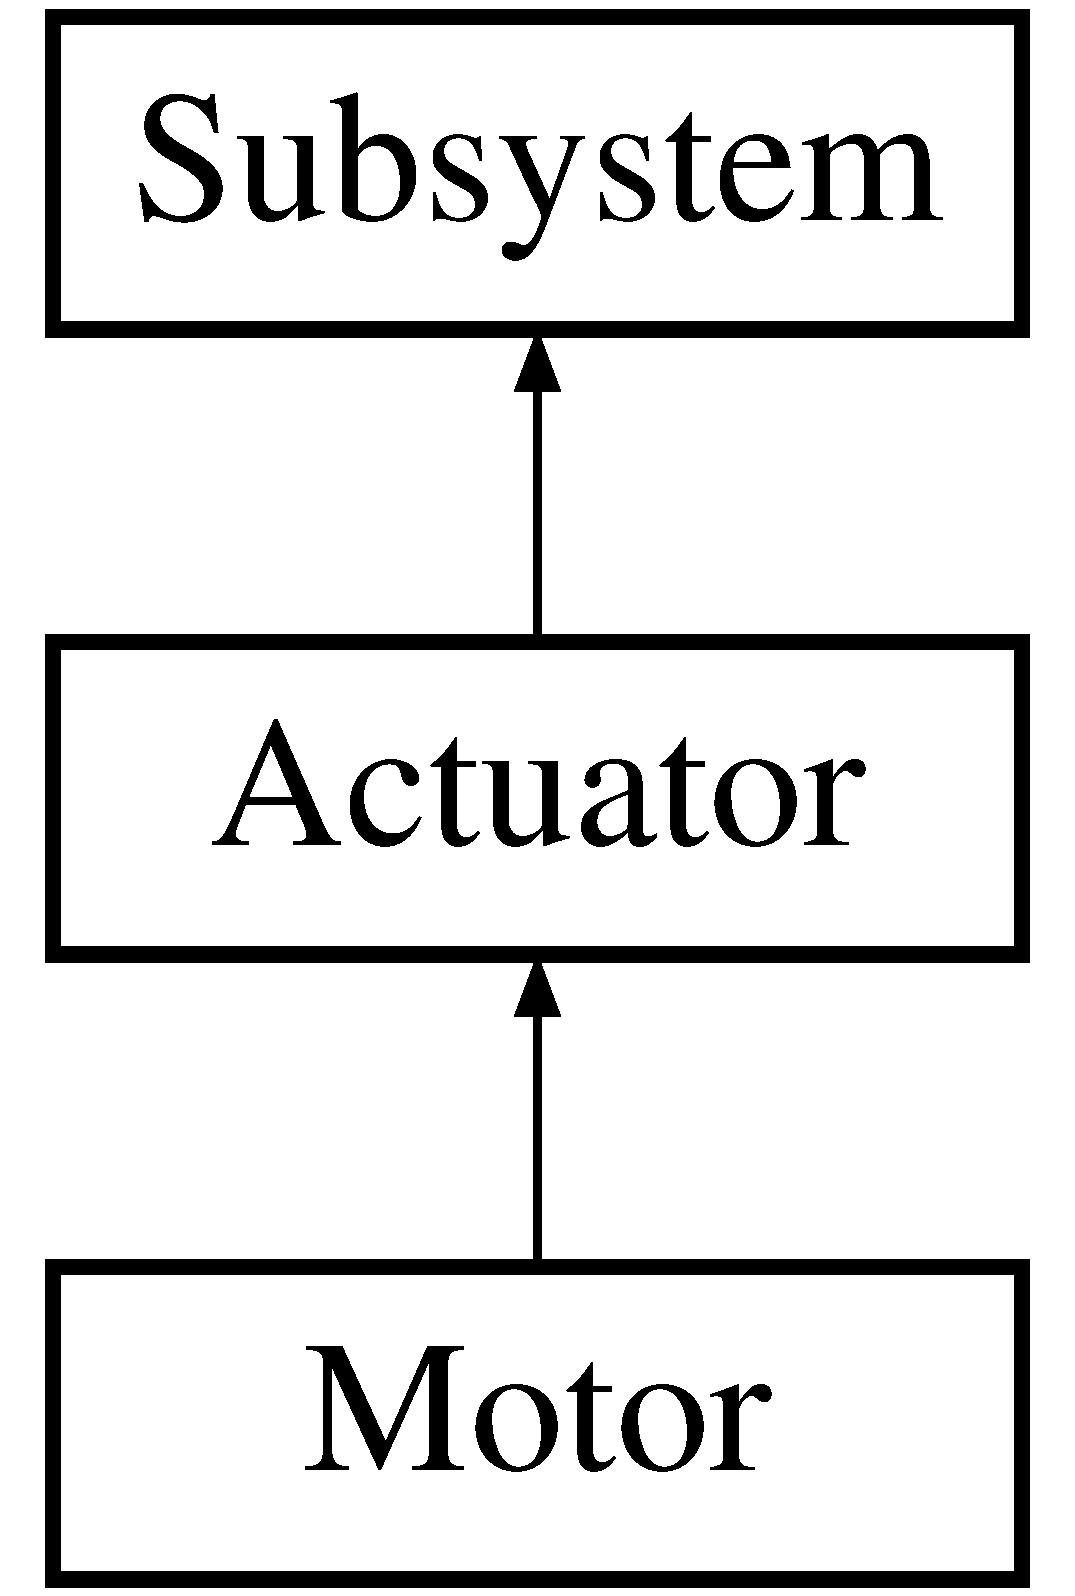
\includegraphics[height=3.000000cm]{classMotor}
\end{center}
\end{figure}
\subsection*{Public Member Functions}
\begin{DoxyCompactItemize}
\item 
\hyperlink{classMotor_af6106b4c506411265c5face762b6c004}{Motor} ()
\begin{DoxyCompactList}\small\item\em \hyperlink{classMotor}{Motor} default constructor. \end{DoxyCompactList}\item 
\hyperlink{classMotor_a2e57c7b2681efea1d3b7f253ee88ecd4}{$\sim$\-Motor} ()
\begin{DoxyCompactList}\small\item\em \hyperlink{classMotor}{Motor} destructor. \end{DoxyCompactList}\item 
void \hyperlink{classMotor_a861cd4da09dd25fc02d711a34f25a988}{init\-\_\-device} ()
\begin{DoxyCompactList}\small\item\em initialize the motor \end{DoxyCompactList}\item 
void \hyperlink{classMotor_a9902b2c030a06ca8a4e2f10c3530dbec}{mech\-\_\-control} ()
\begin{DoxyCompactList}\small\item\em the mechanical controller function for the actuator. \end{DoxyCompactList}\item 
void \hyperlink{classMotor_a3edca1dcb0f3df55eccc09ffb14426a4}{mech\-\_\-command} (char $\ast$value)
\begin{DoxyCompactList}\small\item\em The mechanical command function issues commands directly to the motor hardware. \end{DoxyCompactList}\item 
void $\ast$ \hyperlink{classMotor_a1727e2d2dfd483c9c85824915a6aeeb8}{read\-\_\-data} (int command)
\begin{DoxyCompactList}\small\item\em Reads in data from message to the motor. \end{DoxyCompactList}\item 
void \hyperlink{classMotor_add07c258d9b239633a3882a07dc9e4de}{handle\-\_\-message} (\hyperlink{SUBSYS__COMMANDS_8h_ad814416fc1a8c675bea2687d96088a8f}{M\-E\-S\-S\-A\-G\-E} $\ast$message)
\begin{DoxyCompactList}\small\item\em Handles message sent to the motor. \end{DoxyCompactList}\end{DoxyCompactItemize}
\subsection*{Protected Member Functions}
\begin{DoxyCompactItemize}
\item 
void \hyperlink{classMotor_af6301006bc0b18d6a4b32d2be0cd93a7}{set\-\_\-new\-\_\-pwm\-\_\-duty\-\_\-cycle} (const char $\ast$value)
\begin{DoxyCompactList}\small\item\em Sets the motor P\-W\-M duty cycle. \end{DoxyCompactList}\end{DoxyCompactItemize}
\subsection*{Protected Attributes}
\begin{DoxyCompactItemize}
\item 
int \hyperlink{classMotor_a0125717053068acb08b430d820bfc413}{min\-\_\-priority}
\item 
char \hyperlink{classMotor_a158ba3b940abdc85c7c1e4b1bf651a6e}{motor\-\_\-duty\-\_\-cycle} \mbox{[}6\mbox{]}
\item 
int \hyperlink{classMotor_a7d7c98b5afa45656905708e54ff7fb9a}{direction}
\item 
sem\-\_\-t \hyperlink{classMotor_a827a1d2b453a804d389cdafbf0685022}{motor\-\_\-cmd\-\_\-ctrl}
\item 
int \hyperlink{classMotor_acb2ac1bd2630b05c40a64154a87ea65d}{motor\-\_\-fd}
\item 
char \hyperlink{classMotor_aed42ebef60a1374fc86dd2aff59af85e}{motor\-\_\-filepath} \mbox{[}40\mbox{]}
\item 
\hyperlink{SUBSYS__COMMANDS_8h_ad814416fc1a8c675bea2687d96088a8f}{M\-E\-S\-S\-A\-G\-E} \hyperlink{classMotor_ab2774f3d9c41683a683f10ef20a29607}{data\-\_\-request}
\end{DoxyCompactItemize}
\subsection*{Additional Inherited Members}


\subsection{Detailed Description}
motor control 

receives motor control commands and commands the motor accordingly 

\subsection{Constructor \& Destructor Documentation}
\hypertarget{classMotor_af6106b4c506411265c5face762b6c004}{\index{Motor@{Motor}!Motor@{Motor}}
\index{Motor@{Motor}!Motor@{Motor}}
\subsubsection[{Motor}]{\setlength{\rightskip}{0pt plus 5cm}Motor\-::\-Motor (
\begin{DoxyParamCaption}
{}
\end{DoxyParamCaption}
)}}\label{classMotor_af6106b4c506411265c5face762b6c004}


\hyperlink{classMotor}{Motor} default constructor. 

sets subsystem parameters and sets up the motor command-\/control sync semaphore \hypertarget{classMotor_a2e57c7b2681efea1d3b7f253ee88ecd4}{\index{Motor@{Motor}!$\sim$\-Motor@{$\sim$\-Motor}}
\index{$\sim$\-Motor@{$\sim$\-Motor}!Motor@{Motor}}
\subsubsection[{$\sim$\-Motor}]{\setlength{\rightskip}{0pt plus 5cm}Motor\-::$\sim$\-Motor (
\begin{DoxyParamCaption}
{}
\end{DoxyParamCaption}
)}}\label{classMotor_a2e57c7b2681efea1d3b7f253ee88ecd4}


\hyperlink{classMotor}{Motor} destructor. 

closes the motor file descriptor (P\-W\-M file descriptor) 

\subsection{Member Function Documentation}
\hypertarget{classMotor_add07c258d9b239633a3882a07dc9e4de}{\index{Motor@{Motor}!handle\-\_\-message@{handle\-\_\-message}}
\index{handle\-\_\-message@{handle\-\_\-message}!Motor@{Motor}}
\subsubsection[{handle\-\_\-message}]{\setlength{\rightskip}{0pt plus 5cm}void Motor\-::handle\-\_\-message (
\begin{DoxyParamCaption}
\item[{{\bf M\-E\-S\-S\-A\-G\-E} $\ast$}]{message}
\end{DoxyParamCaption}
)\hspace{0.3cm}{\ttfamily [virtual]}}}\label{classMotor_add07c258d9b239633a3882a07dc9e4de}


Handles message sent to the motor. 

Will handle the messages sent to the motor from the system controller. Messages could be from command line interface or from another subsystem. 

Implements \hyperlink{classActuator_a733c6782030e224bcef26161c77a4d96}{Actuator}.

\hypertarget{classMotor_a861cd4da09dd25fc02d711a34f25a988}{\index{Motor@{Motor}!init\-\_\-device@{init\-\_\-device}}
\index{init\-\_\-device@{init\-\_\-device}!Motor@{Motor}}
\subsubsection[{init\-\_\-device}]{\setlength{\rightskip}{0pt plus 5cm}void Motor\-::init\-\_\-device (
\begin{DoxyParamCaption}
{}
\end{DoxyParamCaption}
)\hspace{0.3cm}{\ttfamily [virtual]}}}\label{classMotor_a861cd4da09dd25fc02d711a34f25a988}


initialize the motor 

Responsible for setting the motor up for control by the mechanical control task. The init\-\_\-device function will set up the P\-W\-M, initialize the system variables, and perform other tasks necessary before the motor can be controlled. 

Implements \hyperlink{classActuator_a13e33ed9c5e19a52bc6d0b7e3c0dd2d7}{Actuator}.

\hypertarget{classMotor_a3edca1dcb0f3df55eccc09ffb14426a4}{\index{Motor@{Motor}!mech\-\_\-command@{mech\-\_\-command}}
\index{mech\-\_\-command@{mech\-\_\-command}!Motor@{Motor}}
\subsubsection[{mech\-\_\-command}]{\setlength{\rightskip}{0pt plus 5cm}void Motor\-::mech\-\_\-command (
\begin{DoxyParamCaption}
\item[{char $\ast$}]{value}
\end{DoxyParamCaption}
)\hspace{0.3cm}{\ttfamily [virtual]}}}\label{classMotor_a3edca1dcb0f3df55eccc09ffb14426a4}


The mechanical command function issues commands directly to the motor hardware. 

The mechanical command function is typically called from the mech\-\_\-control function and will issue the actual commands to hardware necessary to control the motor. This function will write to P\-W\-M to control the motor speed and direction. 

Implements \hyperlink{classActuator_ad9c31f9e7f06684835ae526f29d7a096}{Actuator}.

\hypertarget{classMotor_a9902b2c030a06ca8a4e2f10c3530dbec}{\index{Motor@{Motor}!mech\-\_\-control@{mech\-\_\-control}}
\index{mech\-\_\-control@{mech\-\_\-control}!Motor@{Motor}}
\subsubsection[{mech\-\_\-control}]{\setlength{\rightskip}{0pt plus 5cm}void Motor\-::mech\-\_\-control (
\begin{DoxyParamCaption}
{}
\end{DoxyParamCaption}
)\hspace{0.3cm}{\ttfamily [virtual]}}}\label{classMotor_a9902b2c030a06ca8a4e2f10c3530dbec}


the mechanical controller function for the actuator. 

Runs in the mech\-\_\-control thread and waits for a sync semaphore before issuing a mechanical command if the motor subsystem is enabled. 

Implements \hyperlink{classActuator_a05dd923b5162ebad197fc04d07d9771f}{Actuator}.

\hypertarget{classMotor_a1727e2d2dfd483c9c85824915a6aeeb8}{\index{Motor@{Motor}!read\-\_\-data@{read\-\_\-data}}
\index{read\-\_\-data@{read\-\_\-data}!Motor@{Motor}}
\subsubsection[{read\-\_\-data}]{\setlength{\rightskip}{0pt plus 5cm}void $\ast$ Motor\-::read\-\_\-data (
\begin{DoxyParamCaption}
\item[{int}]{command}
\end{DoxyParamCaption}
)\hspace{0.3cm}{\ttfamily [virtual]}}}\label{classMotor_a1727e2d2dfd483c9c85824915a6aeeb8}


Reads in data from message to the motor. 

Will read data into appropriate data type and then cast to a void$\ast$ and return. The type of data received depends on the message command. For example if trying to set the motor pwm duty cycle, a three byte char$\ast$ is expected. This function will read the data in from standard in (using cin) into an appropriate datatype for the given command and will return the data to the system message handler for further processing. 

Implements \hyperlink{classActuator_a65fe83ffd7895f3ab028b87a62b3af1d}{Actuator}.

\hypertarget{classMotor_af6301006bc0b18d6a4b32d2be0cd93a7}{\index{Motor@{Motor}!set\-\_\-new\-\_\-pwm\-\_\-duty\-\_\-cycle@{set\-\_\-new\-\_\-pwm\-\_\-duty\-\_\-cycle}}
\index{set\-\_\-new\-\_\-pwm\-\_\-duty\-\_\-cycle@{set\-\_\-new\-\_\-pwm\-\_\-duty\-\_\-cycle}!Motor@{Motor}}
\subsubsection[{set\-\_\-new\-\_\-pwm\-\_\-duty\-\_\-cycle}]{\setlength{\rightskip}{0pt plus 5cm}void Motor\-::set\-\_\-new\-\_\-pwm\-\_\-duty\-\_\-cycle (
\begin{DoxyParamCaption}
\item[{const char $\ast$}]{value}
\end{DoxyParamCaption}
)\hspace{0.3cm}{\ttfamily [protected]}}}\label{classMotor_af6301006bc0b18d6a4b32d2be0cd93a7}


Sets the motor P\-W\-M duty cycle. 

Sets the motor\-\_\-duty\-\_\-cycle and gives the motor\-\_\-cmd\-\_\-ctrl sync semaphore which releases the mech\-\_\-control task. 

\subsection{Member Data Documentation}
\hypertarget{classMotor_ab2774f3d9c41683a683f10ef20a29607}{\index{Motor@{Motor}!data\-\_\-request@{data\-\_\-request}}
\index{data\-\_\-request@{data\-\_\-request}!Motor@{Motor}}
\subsubsection[{data\-\_\-request}]{\setlength{\rightskip}{0pt plus 5cm}{\bf M\-E\-S\-S\-A\-G\-E} Motor\-::data\-\_\-request\hspace{0.3cm}{\ttfamily [protected]}}}\label{classMotor_ab2774f3d9c41683a683f10ef20a29607}
message used to send back data requested by other subsystems (typically sonar) \hypertarget{classMotor_a7d7c98b5afa45656905708e54ff7fb9a}{\index{Motor@{Motor}!direction@{direction}}
\index{direction@{direction}!Motor@{Motor}}
\subsubsection[{direction}]{\setlength{\rightskip}{0pt plus 5cm}int Motor\-::direction\hspace{0.3cm}{\ttfamily [protected]}}}\label{classMotor_a7d7c98b5afa45656905708e54ff7fb9a}
the motor direction (1=forward, 0=reverse) \hypertarget{classMotor_a0125717053068acb08b430d820bfc413}{\index{Motor@{Motor}!min\-\_\-priority@{min\-\_\-priority}}
\index{min\-\_\-priority@{min\-\_\-priority}!Motor@{Motor}}
\subsubsection[{min\-\_\-priority}]{\setlength{\rightskip}{0pt plus 5cm}int Motor\-::min\-\_\-priority\hspace{0.3cm}{\ttfamily [protected]}}}\label{classMotor_a0125717053068acb08b430d820bfc413}
minimum priority for commands from other subsystems. For example if compass has priority 5, sonar has priority 2, and min\-\_\-priority is set to 3, commands from the compass will be ignored and commands from sonar will be accepted. \hypertarget{classMotor_a827a1d2b453a804d389cdafbf0685022}{\index{Motor@{Motor}!motor\-\_\-cmd\-\_\-ctrl@{motor\-\_\-cmd\-\_\-ctrl}}
\index{motor\-\_\-cmd\-\_\-ctrl@{motor\-\_\-cmd\-\_\-ctrl}!Motor@{Motor}}
\subsubsection[{motor\-\_\-cmd\-\_\-ctrl}]{\setlength{\rightskip}{0pt plus 5cm}sem\-\_\-t Motor\-::motor\-\_\-cmd\-\_\-ctrl\hspace{0.3cm}{\ttfamily [protected]}}}\label{classMotor_a827a1d2b453a804d389cdafbf0685022}
the command/control sync semaphore \hypertarget{classMotor_a158ba3b940abdc85c7c1e4b1bf651a6e}{\index{Motor@{Motor}!motor\-\_\-duty\-\_\-cycle@{motor\-\_\-duty\-\_\-cycle}}
\index{motor\-\_\-duty\-\_\-cycle@{motor\-\_\-duty\-\_\-cycle}!Motor@{Motor}}
\subsubsection[{motor\-\_\-duty\-\_\-cycle}]{\setlength{\rightskip}{0pt plus 5cm}char Motor\-::motor\-\_\-duty\-\_\-cycle\mbox{[}6\mbox{]}\hspace{0.3cm}{\ttfamily [protected]}}}\label{classMotor_a158ba3b940abdc85c7c1e4b1bf651a6e}
The current set duty cycle for the motor P\-W\-M \hypertarget{classMotor_acb2ac1bd2630b05c40a64154a87ea65d}{\index{Motor@{Motor}!motor\-\_\-fd@{motor\-\_\-fd}}
\index{motor\-\_\-fd@{motor\-\_\-fd}!Motor@{Motor}}
\subsubsection[{motor\-\_\-fd}]{\setlength{\rightskip}{0pt plus 5cm}int Motor\-::motor\-\_\-fd\hspace{0.3cm}{\ttfamily [protected]}}}\label{classMotor_acb2ac1bd2630b05c40a64154a87ea65d}
the motor file descriptor (for the P\-W\-M device) \hypertarget{classMotor_aed42ebef60a1374fc86dd2aff59af85e}{\index{Motor@{Motor}!motor\-\_\-filepath@{motor\-\_\-filepath}}
\index{motor\-\_\-filepath@{motor\-\_\-filepath}!Motor@{Motor}}
\subsubsection[{motor\-\_\-filepath}]{\setlength{\rightskip}{0pt plus 5cm}char Motor\-::motor\-\_\-filepath\mbox{[}40\mbox{]}\hspace{0.3cm}{\ttfamily [protected]}}}\label{classMotor_aed42ebef60a1374fc86dd2aff59af85e}
the filepath to the P\-W\-M device (in /dev) 

The documentation for this class was generated from the following files\-:\begin{DoxyCompactItemize}
\item 
/home/keith/realtime/Motor.\-h\item 
/home/keith/realtime/Motor.\-cpp\end{DoxyCompactItemize}

\hypertarget{classSensor}{\section{Sensor Class Reference}
\label{classSensor}\index{Sensor@{Sensor}}
}


\hyperlink{classSensor}{Sensor} class manages sensor tasks.  




{\ttfamily \#include $<$Sensor.\-h$>$}

Inheritance diagram for Sensor\-:\begin{figure}[H]
\begin{center}
\leavevmode
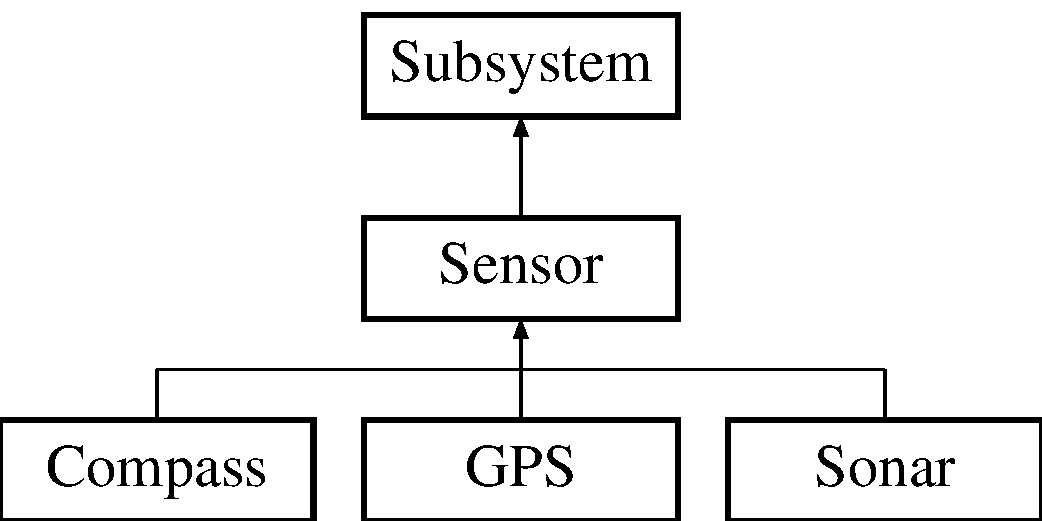
\includegraphics[height=3.000000cm]{classSensor}
\end{center}
\end{figure}
\subsection*{Public Member Functions}
\begin{DoxyCompactItemize}
\item 
\hyperlink{classSensor_a342d6d11ef572c8cba92cb76fb1a294b}{Sensor} ()
\begin{DoxyCompactList}\small\item\em \hyperlink{classSensor}{Sensor} default constructor. \end{DoxyCompactList}\item 
\hyperlink{classSensor_aee8c70e7ef05ce65e7ee33686b5d7db2}{$\sim$\-Sensor} ()
\begin{DoxyCompactList}\small\item\em \hyperlink{classSensor}{Sensor} destructor. \end{DoxyCompactList}\item 
void \hyperlink{classSensor_a84bc35cfba92eb579bc311b3c8b2980d}{init} ()
\begin{DoxyCompactList}\small\item\em initializes the sensor \end{DoxyCompactList}\item 
void \hyperlink{classSensor_a2f08975182e98e644efb226435124047}{shutdown} ()
\begin{DoxyCompactList}\small\item\em shuts down the sensor \end{DoxyCompactList}\item 
virtual void $\ast$ \hyperlink{classSensor_acf4ff5c6c8f793ed47a8105b94ff7c3e}{read\-\_\-data} (int command)=0
\begin{DoxyCompactList}\small\item\em Reads in data from message to the actuator. \end{DoxyCompactList}\item 
virtual void \hyperlink{classSensor_a11b28f6bc91d6f69e734e13ab0e64f56}{init\-\_\-sensor} ()=0
\begin{DoxyCompactList}\small\item\em data grabber \end{DoxyCompactList}\item 
virtual void \hyperlink{classSensor_ae4ec41b880d44feb898da5c62c3203c9}{collector} ()=0
\begin{DoxyCompactList}\small\item\em data collector \end{DoxyCompactList}\item 
virtual void \hyperlink{classSensor_a595d8d9cd87dd3704fad2a313c709a7e}{analysis} ()=0
\begin{DoxyCompactList}\small\item\em data analyzer \end{DoxyCompactList}\item 
virtual void \hyperlink{classSensor_a45533b253f81f85d1b6fcea902a5692b}{handle\-\_\-message} (\hyperlink{SUBSYS__COMMANDS_8h_ad814416fc1a8c675bea2687d96088a8f}{M\-E\-S\-S\-A\-G\-E} $\ast$message)=0
\begin{DoxyCompactList}\small\item\em message handler \end{DoxyCompactList}\end{DoxyCompactItemize}
\subsection*{Protected Attributes}
\begin{DoxyCompactItemize}
\item 
\hypertarget{classSensor_a881761631861338b335680ab1e618277}{pthread\-\_\-t {\bfseries t\-Collector}}\label{classSensor_a881761631861338b335680ab1e618277}

\item 
\hypertarget{classSensor_afce21e3a689654c7d165f2a0e01ab86c}{pthread\-\_\-t {\bfseries t\-Analysis}}\label{classSensor_afce21e3a689654c7d165f2a0e01ab86c}

\item 
\hypertarget{classSensor_af6f47b6f9c15f82dc4f3e92325356763}{int {\bfseries iret\-\_\-\-Collector}}\label{classSensor_af6f47b6f9c15f82dc4f3e92325356763}

\item 
\hypertarget{classSensor_a7227460350eb55d36fae369eda16a774}{int {\bfseries iret\-\_\-\-Analysis}}\label{classSensor_a7227460350eb55d36fae369eda16a774}

\end{DoxyCompactItemize}
\subsection*{Additional Inherited Members}


\subsection{Detailed Description}
\hyperlink{classSensor}{Sensor} class manages sensor tasks. 

Sets up collector and analysis tasks on init and cancels tasks on shutdown 

\subsection{Constructor \& Destructor Documentation}
\hypertarget{classSensor_a342d6d11ef572c8cba92cb76fb1a294b}{\index{Sensor@{Sensor}!Sensor@{Sensor}}
\index{Sensor@{Sensor}!Sensor@{Sensor}}
\subsubsection[{Sensor}]{\setlength{\rightskip}{0pt plus 5cm}Sensor\-::\-Sensor (
\begin{DoxyParamCaption}
{}
\end{DoxyParamCaption}
)\hspace{0.3cm}{\ttfamily [inline]}}}\label{classSensor_a342d6d11ef572c8cba92cb76fb1a294b}


\hyperlink{classSensor}{Sensor} default constructor. 

does nothing \hypertarget{classSensor_aee8c70e7ef05ce65e7ee33686b5d7db2}{\index{Sensor@{Sensor}!$\sim$\-Sensor@{$\sim$\-Sensor}}
\index{$\sim$\-Sensor@{$\sim$\-Sensor}!Sensor@{Sensor}}
\subsubsection[{$\sim$\-Sensor}]{\setlength{\rightskip}{0pt plus 5cm}Sensor\-::$\sim$\-Sensor (
\begin{DoxyParamCaption}
{}
\end{DoxyParamCaption}
)}}\label{classSensor_aee8c70e7ef05ce65e7ee33686b5d7db2}


\hyperlink{classSensor}{Sensor} destructor. 

shuts down the subsystem (cancels the collector and analysis tasks) 

\subsection{Member Function Documentation}
\hypertarget{classSensor_a595d8d9cd87dd3704fad2a313c709a7e}{\index{Sensor@{Sensor}!analysis@{analysis}}
\index{analysis@{analysis}!Sensor@{Sensor}}
\subsubsection[{analysis}]{\setlength{\rightskip}{0pt plus 5cm}virtual void Sensor\-::analysis (
\begin{DoxyParamCaption}
{}
\end{DoxyParamCaption}
)\hspace{0.3cm}{\ttfamily [pure virtual]}}}\label{classSensor_a595d8d9cd87dd3704fad2a313c709a7e}


data analyzer 

virtual fuction defined at the specific sensor level 

Implemented in \hyperlink{classCompass_a4dd6402d0ece9203c6b92670265b4c8d}{Compass}, \hyperlink{classGPS_a4dca50736c5e49f831515219536823b2}{G\-P\-S}, and \hyperlink{classSonar_a11a32c64528f8e69fdde4722f3b3bc7b}{Sonar}.

\hypertarget{classSensor_ae4ec41b880d44feb898da5c62c3203c9}{\index{Sensor@{Sensor}!collector@{collector}}
\index{collector@{collector}!Sensor@{Sensor}}
\subsubsection[{collector}]{\setlength{\rightskip}{0pt plus 5cm}virtual void Sensor\-::collector (
\begin{DoxyParamCaption}
{}
\end{DoxyParamCaption}
)\hspace{0.3cm}{\ttfamily [pure virtual]}}}\label{classSensor_ae4ec41b880d44feb898da5c62c3203c9}


data collector 

virtual fuction defined at the specific sensor level 

Implemented in \hyperlink{classCompass_ae8d7f3417a27b1d18487b96ca07dd32b}{Compass}, \hyperlink{classGPS_a17383568c4ed86a0adfdd5c88b6591d4}{G\-P\-S}, and \hyperlink{classSonar_a38b0e409082be17e7098b2e471bab4a8}{Sonar}.

\hypertarget{classSensor_a45533b253f81f85d1b6fcea902a5692b}{\index{Sensor@{Sensor}!handle\-\_\-message@{handle\-\_\-message}}
\index{handle\-\_\-message@{handle\-\_\-message}!Sensor@{Sensor}}
\subsubsection[{handle\-\_\-message}]{\setlength{\rightskip}{0pt plus 5cm}virtual void Sensor\-::handle\-\_\-message (
\begin{DoxyParamCaption}
\item[{{\bf M\-E\-S\-S\-A\-G\-E} $\ast$}]{message}
\end{DoxyParamCaption}
)\hspace{0.3cm}{\ttfamily [pure virtual]}}}\label{classSensor_a45533b253f81f85d1b6fcea902a5692b}


message handler 

virtual fuction defined at the specific sensor level 

Implements \hyperlink{classSubsystem_a6205bccfd4906044065d25d8ab1a7bfb}{Subsystem}.



Implemented in \hyperlink{classCompass_a1fb0f64b335e8f1d4f27dc2067312b4a}{Compass}, \hyperlink{classGPS_a803a498352e30044136502a9e036d380}{G\-P\-S}, and \hyperlink{classSonar_a5f9b0f57b5a05b03b0dcb5ab830592ff}{Sonar}.

\hypertarget{classSensor_a84bc35cfba92eb579bc311b3c8b2980d}{\index{Sensor@{Sensor}!init@{init}}
\index{init@{init}!Sensor@{Sensor}}
\subsubsection[{init}]{\setlength{\rightskip}{0pt plus 5cm}void Sensor\-::init (
\begin{DoxyParamCaption}
{}
\end{DoxyParamCaption}
)\hspace{0.3cm}{\ttfamily [virtual]}}}\label{classSensor_a84bc35cfba92eb579bc311b3c8b2980d}


initializes the sensor 

starts the collector and anaysis tasks 

Implements \hyperlink{classSubsystem_a77a984e8a06bfebb924a6e7ba4f98363}{Subsystem}.

\hypertarget{classSensor_a11b28f6bc91d6f69e734e13ab0e64f56}{\index{Sensor@{Sensor}!init\-\_\-sensor@{init\-\_\-sensor}}
\index{init\-\_\-sensor@{init\-\_\-sensor}!Sensor@{Sensor}}
\subsubsection[{init\-\_\-sensor}]{\setlength{\rightskip}{0pt plus 5cm}virtual void Sensor\-::init\-\_\-sensor (
\begin{DoxyParamCaption}
{}
\end{DoxyParamCaption}
)\hspace{0.3cm}{\ttfamily [pure virtual]}}}\label{classSensor_a11b28f6bc91d6f69e734e13ab0e64f56}


data grabber 

virtual fuction defined at the specific sensor level that initializes the sensor 

Implemented in \hyperlink{classCompass_a5cc2b71700af542b5aafadea4820a476}{Compass}, \hyperlink{classGPS_aebb999362899800a7e372e873bb5b943}{G\-P\-S}, and \hyperlink{classSonar_af91d04cbc441084ba608a49c2be88d5b}{Sonar}.

\hypertarget{classSensor_acf4ff5c6c8f793ed47a8105b94ff7c3e}{\index{Sensor@{Sensor}!read\-\_\-data@{read\-\_\-data}}
\index{read\-\_\-data@{read\-\_\-data}!Sensor@{Sensor}}
\subsubsection[{read\-\_\-data}]{\setlength{\rightskip}{0pt plus 5cm}virtual void$\ast$ Sensor\-::read\-\_\-data (
\begin{DoxyParamCaption}
\item[{int}]{command}
\end{DoxyParamCaption}
)\hspace{0.3cm}{\ttfamily [pure virtual]}}}\label{classSensor_acf4ff5c6c8f793ed47a8105b94ff7c3e}


Reads in data from message to the actuator. 

Virtual function implemented at the subsystem level. Will read data into appropriate data type and then cast to a void$\ast$ and return. The type of data received depends on the message command. For example if trying to set the motor pwm duty cycle, a three byte char$\ast$ is expected. This function will read the data in from standard in (using cin) into an appropriate datatype for the given command and will return the data to the system message handler for further processing. 

Implements \hyperlink{classSubsystem_a85307df3e46421814204f77929e893aa}{Subsystem}.



Implemented in \hyperlink{classCompass_ab55d084e2d643df0a1970f5868d0c5a8}{Compass}, \hyperlink{classGPS_aa04076536ee9f7e2679895c69b07ad58}{G\-P\-S}, and \hyperlink{classSonar_a54f55470741873f333ad8af8a98affc8}{Sonar}.

\hypertarget{classSensor_a2f08975182e98e644efb226435124047}{\index{Sensor@{Sensor}!shutdown@{shutdown}}
\index{shutdown@{shutdown}!Sensor@{Sensor}}
\subsubsection[{shutdown}]{\setlength{\rightskip}{0pt plus 5cm}void Sensor\-::shutdown (
\begin{DoxyParamCaption}
{}
\end{DoxyParamCaption}
)\hspace{0.3cm}{\ttfamily [virtual]}}}\label{classSensor_a2f08975182e98e644efb226435124047}


shuts down the sensor 

cancels the collector and analysis tasks 

Implements \hyperlink{classSubsystem_a510e18f972a3d86d7a47432dafa1ce4c}{Subsystem}.



The documentation for this class was generated from the following files\-:\begin{DoxyCompactItemize}
\item 
/home/keith/realtime/Sensor.\-h\item 
/home/keith/realtime/Sensor.\-cpp\end{DoxyCompactItemize}

\hypertarget{classSonar}{\section{Sonar Class Reference}
\label{classSonar}\index{Sonar@{Sonar}}
}


sonar data collection and analysis  




{\ttfamily \#include $<$Sonar.\-h$>$}

Inheritance diagram for Sonar\-:\begin{figure}[H]
\begin{center}
\leavevmode
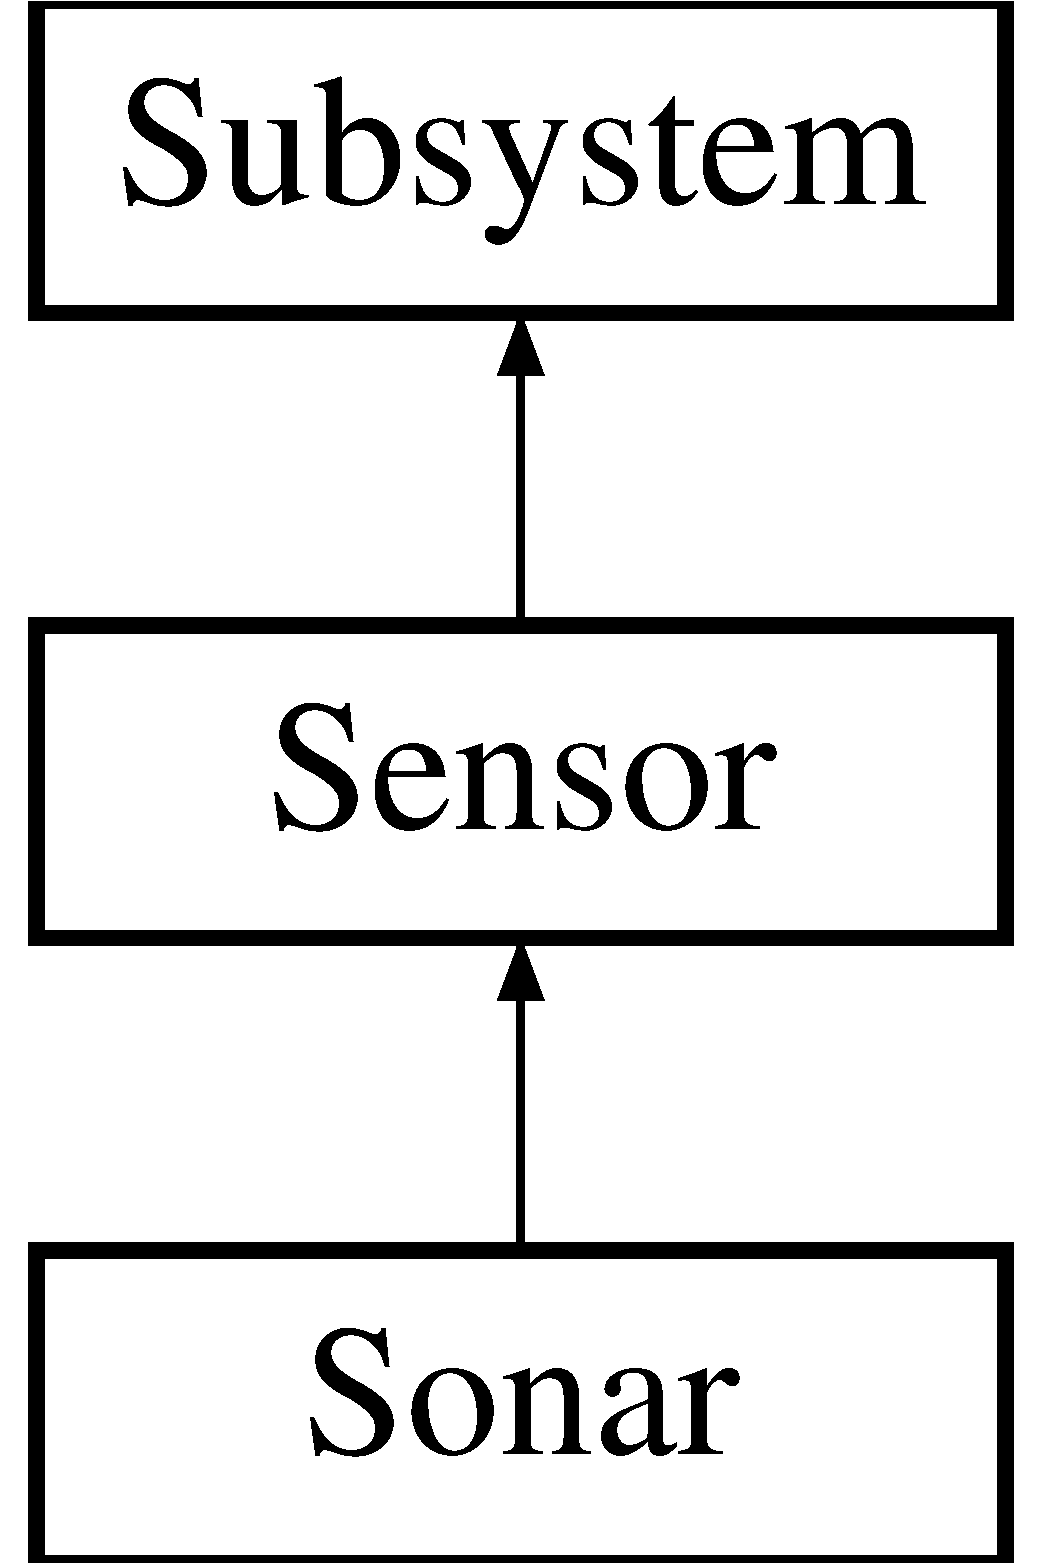
\includegraphics[height=3.000000cm]{classSonar}
\end{center}
\end{figure}
\subsection*{Public Member Functions}
\begin{DoxyCompactItemize}
\item 
\hyperlink{classSonar_a71ef009d138f1e372fc35ca0cb6e85e2}{Sonar} ()
\begin{DoxyCompactList}\small\item\em sonar default constructor \end{DoxyCompactList}\item 
float \hyperlink{classSonar_aa4e807cbed15ce1d46ddcef05b6b59fb}{data\-\_\-grab} ()
\begin{DoxyCompactList}\small\item\em grabs data from sonar \end{DoxyCompactList}\item 
void \hyperlink{classSonar_af91d04cbc441084ba608a49c2be88d5b}{init\-\_\-sensor} ()
\begin{DoxyCompactList}\small\item\em Initializes the \hyperlink{classSonar}{Sonar} subsystem. \end{DoxyCompactList}\item 
void \hyperlink{classSonar_a38b0e409082be17e7098b2e471bab4a8}{collector} ()
\begin{DoxyCompactList}\small\item\em collects data from \hyperlink{classSonar}{Sonar} \end{DoxyCompactList}\item 
void \hyperlink{classSonar_a11a32c64528f8e69fdde4722f3b3bc7b}{analysis} ()
\begin{DoxyCompactList}\small\item\em Performs the analysis of the data collected from the sonar and commands the actuators. \end{DoxyCompactList}\item 
void $\ast$ \hyperlink{classSonar_a54f55470741873f333ad8af8a98affc8}{read\-\_\-data} (int command)
\begin{DoxyCompactList}\small\item\em Reads in data from message to \hyperlink{classSonar}{Sonar}. \end{DoxyCompactList}\item 
void \hyperlink{classSonar_a5f9b0f57b5a05b03b0dcb5ab830592ff}{handle\-\_\-message} (\hyperlink{SUBSYS__COMMANDS_8h_ad814416fc1a8c675bea2687d96088a8f}{M\-E\-S\-S\-A\-G\-E} $\ast$message)
\begin{DoxyCompactList}\small\item\em Handles messages sent to the sonar subsystem. \end{DoxyCompactList}\end{DoxyCompactItemize}
\subsection*{Protected Attributes}
\begin{DoxyCompactItemize}
\item 
float \hyperlink{classSonar_abd3f8ccfc42cacd700df9be06f70c6b2}{sonar\-\_\-reading}
\item 
sem\-\_\-t \hyperlink{classSonar_a3dcf7c38af34539c68f123f073eb2f52}{collect\-\_\-analysis\-\_\-sync}
\item 
int \hyperlink{classSonar_a4799c8b328d7735f7e6d62d741340c6c}{sonar\-\_\-fd}
\item 
char \hyperlink{classSonar_a7db9106da9a50d06b5f25c35f799abe5}{sonar\-\_\-filepath} \mbox{[}40\mbox{]}
\end{DoxyCompactItemize}
\subsection*{Additional Inherited Members}


\subsection{Detailed Description}
sonar data collection and analysis 

Collects data from the sonar and analyzes the data. Based on analysis of collected data, sends messages (using the system message queue) to the control actuators (\hyperlink{classSteering}{Steering} and \hyperlink{classMotor}{Motor}). 

\subsection{Constructor \& Destructor Documentation}
\hypertarget{classSonar_a71ef009d138f1e372fc35ca0cb6e85e2}{\index{Sonar@{Sonar}!Sonar@{Sonar}}
\index{Sonar@{Sonar}!Sonar@{Sonar}}
\subsubsection[{Sonar}]{\setlength{\rightskip}{0pt plus 5cm}Sonar\-::\-Sonar (
\begin{DoxyParamCaption}
{}
\end{DoxyParamCaption}
)}}\label{classSonar_a71ef009d138f1e372fc35ca0cb6e85e2}


sonar default constructor 

sets subsystem parameters and sets up the collect/analysis task sync semaphore. 

\subsection{Member Function Documentation}
\hypertarget{classSonar_a11a32c64528f8e69fdde4722f3b3bc7b}{\index{Sonar@{Sonar}!analysis@{analysis}}
\index{analysis@{analysis}!Sonar@{Sonar}}
\subsubsection[{analysis}]{\setlength{\rightskip}{0pt plus 5cm}void Sonar\-::analysis (
\begin{DoxyParamCaption}
{}
\end{DoxyParamCaption}
)\hspace{0.3cm}{\ttfamily [virtual]}}}\label{classSonar_a11a32c64528f8e69fdde4722f3b3bc7b}


Performs the analysis of the data collected from the sonar and commands the actuators. 

The analysis function executes in the analysis thread and is synced with the collector task by the collect\-\_\-analysis\-\_\-sync semaphore. Depending on the distance reading from the sonar hardware, messages will be sent to the \hyperlink{classMotor}{Motor} and \hyperlink{classSteering}{Steering} subsystems using the system message queue to change course. 

Implements \hyperlink{classSensor_a595d8d9cd87dd3704fad2a313c709a7e}{Sensor}.

\hypertarget{classSonar_a38b0e409082be17e7098b2e471bab4a8}{\index{Sonar@{Sonar}!collector@{collector}}
\index{collector@{collector}!Sonar@{Sonar}}
\subsubsection[{collector}]{\setlength{\rightskip}{0pt plus 5cm}void Sonar\-::collector (
\begin{DoxyParamCaption}
{}
\end{DoxyParamCaption}
)\hspace{0.3cm}{\ttfamily [virtual]}}}\label{classSonar_a38b0e409082be17e7098b2e471bab4a8}


collects data from \hyperlink{classSonar}{Sonar} 

The collector function executes in the collector thread and executes indefinitely at a frequency of 20\-Hz. It calls the data\-\_\-grab to do the actual communication with the hardware to provide a layer of abstraction between the software and specifics of the hardware. It can optionally average data prior to analysis if the system is expected to be under heavy load and the tasks are not schedulable with the typical release frequencies (averaging will have the effect that the analysis task will be released less frequently). 

Implements \hyperlink{classSensor_ae4ec41b880d44feb898da5c62c3203c9}{Sensor}.

\hypertarget{classSonar_aa4e807cbed15ce1d46ddcef05b6b59fb}{\index{Sonar@{Sonar}!data\-\_\-grab@{data\-\_\-grab}}
\index{data\-\_\-grab@{data\-\_\-grab}!Sonar@{Sonar}}
\subsubsection[{data\-\_\-grab}]{\setlength{\rightskip}{0pt plus 5cm}float Sonar\-::data\-\_\-grab (
\begin{DoxyParamCaption}
{}
\end{DoxyParamCaption}
)}}\label{classSonar_aa4e807cbed15ce1d46ddcef05b6b59fb}


grabs data from sonar 

Gets data from sonar over S\-P\-I. Returns a distance as a float. \hypertarget{classSonar_a5f9b0f57b5a05b03b0dcb5ab830592ff}{\index{Sonar@{Sonar}!handle\-\_\-message@{handle\-\_\-message}}
\index{handle\-\_\-message@{handle\-\_\-message}!Sonar@{Sonar}}
\subsubsection[{handle\-\_\-message}]{\setlength{\rightskip}{0pt plus 5cm}void Sonar\-::handle\-\_\-message (
\begin{DoxyParamCaption}
\item[{{\bf M\-E\-S\-S\-A\-G\-E} $\ast$}]{message}
\end{DoxyParamCaption}
)\hspace{0.3cm}{\ttfamily [virtual]}}}\label{classSonar_a5f9b0f57b5a05b03b0dcb5ab830592ff}


Handles messages sent to the sonar subsystem. 

Performs tasks determined by the command part of the message. For example the command S\-N\-R\-\_\-\-S\-E\-T\-\_\-\-D\-I\-S\-T\-\_\-\-T\-H\-R is used to set the distance threshold. Messages could be from command line interface or from another subsystem. 

Implements \hyperlink{classSensor_a45533b253f81f85d1b6fcea902a5692b}{Sensor}.

\hypertarget{classSonar_af91d04cbc441084ba608a49c2be88d5b}{\index{Sonar@{Sonar}!init\-\_\-sensor@{init\-\_\-sensor}}
\index{init\-\_\-sensor@{init\-\_\-sensor}!Sonar@{Sonar}}
\subsubsection[{init\-\_\-sensor}]{\setlength{\rightskip}{0pt plus 5cm}void Sonar\-::init\-\_\-sensor (
\begin{DoxyParamCaption}
{}
\end{DoxyParamCaption}
)\hspace{0.3cm}{\ttfamily [virtual]}}}\label{classSonar_af91d04cbc441084ba608a49c2be88d5b}


Initializes the \hyperlink{classSonar}{Sonar} subsystem. 

Sets up the S\-P\-I driver (to talk to the A\-D\-C) and sets up the A\-D\-C for sonar configuration. 

Implements \hyperlink{classSensor_a11b28f6bc91d6f69e734e13ab0e64f56}{Sensor}.

\hypertarget{classSonar_a54f55470741873f333ad8af8a98affc8}{\index{Sonar@{Sonar}!read\-\_\-data@{read\-\_\-data}}
\index{read\-\_\-data@{read\-\_\-data}!Sonar@{Sonar}}
\subsubsection[{read\-\_\-data}]{\setlength{\rightskip}{0pt plus 5cm}void $\ast$ Sonar\-::read\-\_\-data (
\begin{DoxyParamCaption}
\item[{int}]{command}
\end{DoxyParamCaption}
)\hspace{0.3cm}{\ttfamily [virtual]}}}\label{classSonar_a54f55470741873f333ad8af8a98affc8}


Reads in data from message to \hyperlink{classSonar}{Sonar}. 

Will read data into appropriate data type and then cast to a void$\ast$ and return. The type of data received depends on the message command. For example if trying to set the threashold distance, an int is expected. This function will read the data in from standard in (using cin) into an appropriate datatype for the given command and will return the data to the system message handler for further processing. 

Implements \hyperlink{classSensor_acf4ff5c6c8f793ed47a8105b94ff7c3e}{Sensor}.



\subsection{Member Data Documentation}
\hypertarget{classSonar_a3dcf7c38af34539c68f123f073eb2f52}{\index{Sonar@{Sonar}!collect\-\_\-analysis\-\_\-sync@{collect\-\_\-analysis\-\_\-sync}}
\index{collect\-\_\-analysis\-\_\-sync@{collect\-\_\-analysis\-\_\-sync}!Sonar@{Sonar}}
\subsubsection[{collect\-\_\-analysis\-\_\-sync}]{\setlength{\rightskip}{0pt plus 5cm}sem\-\_\-t Sonar\-::collect\-\_\-analysis\-\_\-sync\hspace{0.3cm}{\ttfamily [protected]}}}\label{classSonar_a3dcf7c38af34539c68f123f073eb2f52}
the colector/analysis sync semaphore used to sync the collector and analysis tasks \hypertarget{classSonar_a4799c8b328d7735f7e6d62d741340c6c}{\index{Sonar@{Sonar}!sonar\-\_\-fd@{sonar\-\_\-fd}}
\index{sonar\-\_\-fd@{sonar\-\_\-fd}!Sonar@{Sonar}}
\subsubsection[{sonar\-\_\-fd}]{\setlength{\rightskip}{0pt plus 5cm}int Sonar\-::sonar\-\_\-fd\hspace{0.3cm}{\ttfamily [protected]}}}\label{classSonar_a4799c8b328d7735f7e6d62d741340c6c}
The sonar file descriptor (S\-P\-I file descriptor) \hypertarget{classSonar_a7db9106da9a50d06b5f25c35f799abe5}{\index{Sonar@{Sonar}!sonar\-\_\-filepath@{sonar\-\_\-filepath}}
\index{sonar\-\_\-filepath@{sonar\-\_\-filepath}!Sonar@{Sonar}}
\subsubsection[{sonar\-\_\-filepath}]{\setlength{\rightskip}{0pt plus 5cm}char Sonar\-::sonar\-\_\-filepath\mbox{[}40\mbox{]}\hspace{0.3cm}{\ttfamily [protected]}}}\label{classSonar_a7db9106da9a50d06b5f25c35f799abe5}
filepath for the S\-P\-I device (in /dev) \hypertarget{classSonar_abd3f8ccfc42cacd700df9be06f70c6b2}{\index{Sonar@{Sonar}!sonar\-\_\-reading@{sonar\-\_\-reading}}
\index{sonar\-\_\-reading@{sonar\-\_\-reading}!Sonar@{Sonar}}
\subsubsection[{sonar\-\_\-reading}]{\setlength{\rightskip}{0pt plus 5cm}float Sonar\-::sonar\-\_\-reading\hspace{0.3cm}{\ttfamily [protected]}}}\label{classSonar_abd3f8ccfc42cacd700df9be06f70c6b2}
The most recent sonar reading 

The documentation for this class was generated from the following files\-:\begin{DoxyCompactItemize}
\item 
/home/keith/realtime/Sonar.\-h\item 
/home/keith/realtime/Sonar.\-cpp\end{DoxyCompactItemize}

\hypertarget{classSteering}{\section{Steering Class Reference}
\label{classSteering}\index{Steering@{Steering}}
}


\hyperlink{classSteering}{Steering} control.  




{\ttfamily \#include $<$Steering.\-h$>$}

Inheritance diagram for Steering\-:\begin{figure}[H]
\begin{center}
\leavevmode
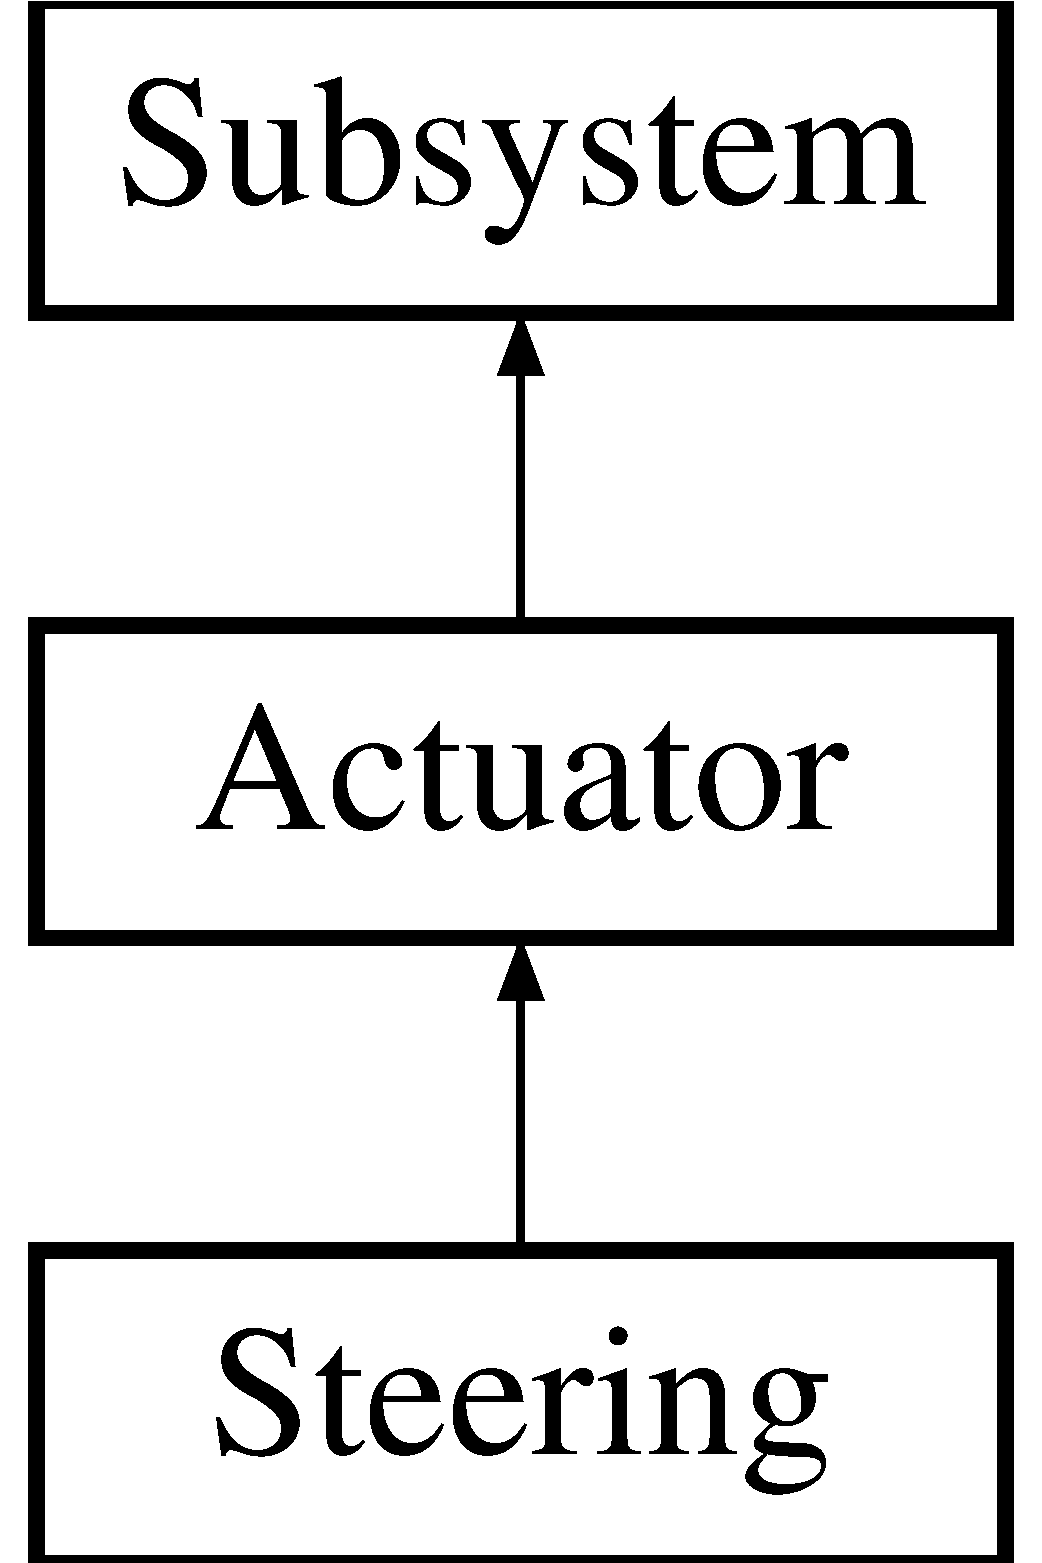
\includegraphics[height=3.000000cm]{classSteering}
\end{center}
\end{figure}
\subsection*{Public Member Functions}
\begin{DoxyCompactItemize}
\item 
\hyperlink{classSteering_a45a5ff1a1869073a2165680f853b9c41}{Steering} ()
\begin{DoxyCompactList}\small\item\em \hyperlink{classActuator}{Actuator} default constructor. \end{DoxyCompactList}\item 
void \hyperlink{classSteering_a57a8011d7d5a4ca608b1b140e21233cb}{init\-\_\-device} ()
\begin{DoxyCompactList}\small\item\em Virtual function to initialize the actuator device. \end{DoxyCompactList}\item 
\hypertarget{classSteering_a5b7b0a053607ad891b7d2826093da6ac}{void \hyperlink{classSteering_a5b7b0a053607ad891b7d2826093da6ac}{mech\-\_\-control} ()}\label{classSteering_a5b7b0a053607ad891b7d2826093da6ac}

\begin{DoxyCompactList}\small\item\em controls the mechanical system \end{DoxyCompactList}\item 
void \hyperlink{classSteering_a0ae09490e872d21d211ddfdc446d14d1}{mech\-\_\-command} (char $\ast$value)
\begin{DoxyCompactList}\small\item\em The mechanical command function issues commands directly to hardware. \end{DoxyCompactList}\item 
void $\ast$ \hyperlink{classSteering_afda4f2951e5be114abf988a8e5943a96}{read\-\_\-data} (int command)
\begin{DoxyCompactList}\small\item\em Reads in data from message to the actuator. \end{DoxyCompactList}\item 
\hypertarget{classSteering_a29e46d1b87ecda7807452ad67005efe1}{void \hyperlink{classSteering_a29e46d1b87ecda7807452ad67005efe1}{handle\-\_\-message} (\hyperlink{SUBSYS__COMMANDS_8h_ad814416fc1a8c675bea2687d96088a8f}{M\-E\-S\-S\-A\-G\-E} $\ast$message)}\label{classSteering_a29e46d1b87ecda7807452ad67005efe1}

\begin{DoxyCompactList}\small\item\em handles messages sent to the compass subsystem \end{DoxyCompactList}\end{DoxyCompactItemize}
\subsection*{Protected Member Functions}
\begin{DoxyCompactItemize}
\item 
\hypertarget{classSteering_aa0f0e87b925f860575429668a9a84e8d}{void {\bfseries set\-\_\-new\-\_\-pwm\-\_\-duty\-\_\-cycle} (const char $\ast$value)}\label{classSteering_aa0f0e87b925f860575429668a9a84e8d}

\end{DoxyCompactItemize}
\subsection*{Protected Attributes}
\begin{DoxyCompactItemize}
\item 
\hypertarget{classSteering_ab31761e4665bf81e580f1bc32c9fff79}{int {\bfseries min\-\_\-priority}}\label{classSteering_ab31761e4665bf81e580f1bc32c9fff79}

\item 
\hypertarget{classSteering_a3eb0bda8706c97d35c0ae31daeefa5a1}{char {\bfseries steering\-\_\-duty\-\_\-cycle} \mbox{[}2\mbox{]}}\label{classSteering_a3eb0bda8706c97d35c0ae31daeefa5a1}

\item 
\hypertarget{classSteering_af9a4f30e9dc0dc37b31a421cb88ca8ba}{sem\-\_\-t {\bfseries steer\-\_\-cmd\-\_\-ctrl}}\label{classSteering_af9a4f30e9dc0dc37b31a421cb88ca8ba}

\item 
\hypertarget{classSteering_ae85b07902746525a57bf049d872b4f26}{int {\bfseries steering\-\_\-fd}}\label{classSteering_ae85b07902746525a57bf049d872b4f26}

\item 
\hypertarget{classSteering_adfe05011b3442b1b24cd9dfc1e24ad70}{char {\bfseries steering\-\_\-filepath} \mbox{[}40\mbox{]}}\label{classSteering_adfe05011b3442b1b24cd9dfc1e24ad70}

\item 
\hypertarget{classSteering_a7182316ec06b0de5008653868d9fdb07}{volatile uint32\-\_\-t $\ast$ {\bfseries gptimer\-\_\-reg}}\label{classSteering_a7182316ec06b0de5008653868d9fdb07}

\end{DoxyCompactItemize}
\subsection*{Additional Inherited Members}


\subsection{Detailed Description}
\hyperlink{classSteering}{Steering} control. 

receives steering control commands and commands the servo accordingly 

\subsection{Constructor \& Destructor Documentation}
\hypertarget{classSteering_a45a5ff1a1869073a2165680f853b9c41}{\index{Steering@{Steering}!Steering@{Steering}}
\index{Steering@{Steering}!Steering@{Steering}}
\subsubsection[{Steering}]{\setlength{\rightskip}{0pt plus 5cm}Steering\-::\-Steering (
\begin{DoxyParamCaption}
{}
\end{DoxyParamCaption}
)}}\label{classSteering_a45a5ff1a1869073a2165680f853b9c41}


\hyperlink{classActuator}{Actuator} default constructor. 

sets subsystem parameters 

\subsection{Member Function Documentation}
\hypertarget{classSteering_a57a8011d7d5a4ca608b1b140e21233cb}{\index{Steering@{Steering}!init\-\_\-device@{init\-\_\-device}}
\index{init\-\_\-device@{init\-\_\-device}!Steering@{Steering}}
\subsubsection[{init\-\_\-device}]{\setlength{\rightskip}{0pt plus 5cm}void Steering\-::init\-\_\-device (
\begin{DoxyParamCaption}
{}
\end{DoxyParamCaption}
)\hspace{0.3cm}{\ttfamily [virtual]}}}\label{classSteering_a57a8011d7d5a4ca608b1b140e21233cb}


Virtual function to initialize the actuator device. 

Defined for each actuator, the init\-\_\-device function is responsible for setting the actuator up for control by the mechanical control task. For example in the case of the motor subsystem, the init\-\_\-device task will set up the P\-W\-M, initialize the system variables, and perform other tasks necessary before the motor can be controlled. 

Implements \hyperlink{classActuator_a13e33ed9c5e19a52bc6d0b7e3c0dd2d7}{Actuator}.

\hypertarget{classSteering_a0ae09490e872d21d211ddfdc446d14d1}{\index{Steering@{Steering}!mech\-\_\-command@{mech\-\_\-command}}
\index{mech\-\_\-command@{mech\-\_\-command}!Steering@{Steering}}
\subsubsection[{mech\-\_\-command}]{\setlength{\rightskip}{0pt plus 5cm}void Steering\-::mech\-\_\-command (
\begin{DoxyParamCaption}
\item[{char $\ast$}]{value}
\end{DoxyParamCaption}
)\hspace{0.3cm}{\ttfamily [virtual]}}}\label{classSteering_a0ae09490e872d21d211ddfdc446d14d1}


The mechanical command function issues commands directly to hardware. 

The mechanical command function is typically called from the mech\-\_\-control function and will issue the actual commands to hardware necessary to control the actuator. For example, for the motor subsystem, this function will write to P\-W\-M. 

Implements \hyperlink{classActuator_ad9c31f9e7f06684835ae526f29d7a096}{Actuator}.

\hypertarget{classSteering_afda4f2951e5be114abf988a8e5943a96}{\index{Steering@{Steering}!read\-\_\-data@{read\-\_\-data}}
\index{read\-\_\-data@{read\-\_\-data}!Steering@{Steering}}
\subsubsection[{read\-\_\-data}]{\setlength{\rightskip}{0pt plus 5cm}void $\ast$ Steering\-::read\-\_\-data (
\begin{DoxyParamCaption}
\item[{int}]{command}
\end{DoxyParamCaption}
)\hspace{0.3cm}{\ttfamily [virtual]}}}\label{classSteering_afda4f2951e5be114abf988a8e5943a96}


Reads in data from message to the actuator. 

Will read data into appropriate data type and then cast to a void$\ast$ and return. The type of data received depends on the message command. For example if trying to set the motor pwm duty cycle, a three byte char$\ast$ is expected. This function will read the data in from standard in (using cin) into an appropriate datatype for the given command and will return the data to the system message handler for further processing. 

Implements \hyperlink{classActuator_a65fe83ffd7895f3ab028b87a62b3af1d}{Actuator}.



The documentation for this class was generated from the following files\-:\begin{DoxyCompactItemize}
\item 
/home/keith/realtime/Steering.\-h\item 
/home/keith/realtime/Steering.\-cpp\end{DoxyCompactItemize}

\input{classsubsys__timing}
\hypertarget{classSubsystem}{\section{Subsystem Class Reference}
\label{classSubsystem}\index{Subsystem@{Subsystem}}
}


The \hyperlink{classSubsystem}{Subsystem} class defines the basic properties shared by all subsystems.  




{\ttfamily \#include $<$Subsystem.\-h$>$}

Inheritance diagram for Subsystem\-:\begin{figure}[H]
\begin{center}
\leavevmode
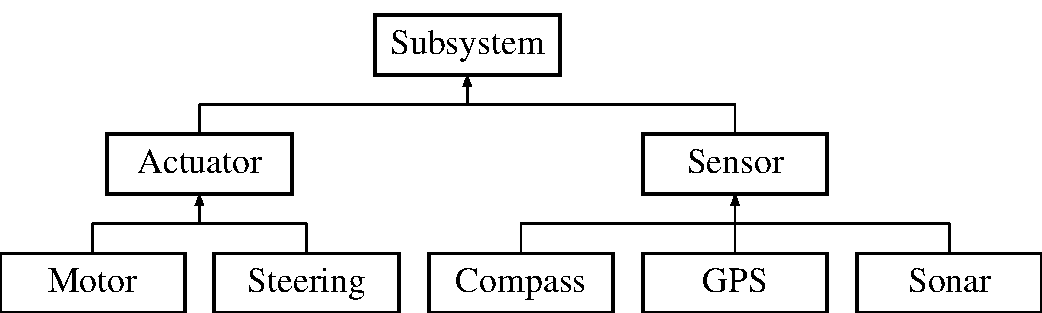
\includegraphics[height=3.000000cm]{classSubsystem}
\end{center}
\end{figure}
\subsection*{Public Member Functions}
\begin{DoxyCompactItemize}
\item 
\hyperlink{classSubsystem_abdec44abe9ddba76f65abb02f8f62992}{Subsystem} ()
\begin{DoxyCompactList}\small\item\em \hyperlink{classSubsystem}{Subsystem} default constructor. \end{DoxyCompactList}\item 
\hyperlink{classSubsystem_af6026d0c678986cf1626251bf38916fa}{$\sim$\-Subsystem} ()
\begin{DoxyCompactList}\small\item\em \hyperlink{classSubsystem}{Subsystem} destructor. \end{DoxyCompactList}\item 
virtual void \hyperlink{classSubsystem_a77a984e8a06bfebb924a6e7ba4f98363}{init} ()=0
\begin{DoxyCompactList}\small\item\em Initializes the subsystem tasks particular to that subsystem. \end{DoxyCompactList}\item 
void \hyperlink{classSubsystem_a2c33b82253ec4588067349e33247f504}{send\-\_\-sys\-\_\-message} (\hyperlink{SUBSYS__COMMANDS_8h_ad814416fc1a8c675bea2687d96088a8f}{M\-E\-S\-S\-A\-G\-E} $\ast$message)
\begin{DoxyCompactList}\small\item\em send message to system \end{DoxyCompactList}\item 
virtual void \hyperlink{classSubsystem_a510e18f972a3d86d7a47432dafa1ce4c}{shutdown} ()=0
\begin{DoxyCompactList}\small\item\em Shutdown subsystem. \end{DoxyCompactList}\item 
virtual void $\ast$ \hyperlink{classSubsystem_a85307df3e46421814204f77929e893aa}{read\-\_\-data} (int command)=0
\begin{DoxyCompactList}\small\item\em Reads in data from message to the actuator. \end{DoxyCompactList}\item 
virtual void \hyperlink{classSubsystem_a6205bccfd4906044065d25d8ab1a7bfb}{handle\-\_\-message} (\hyperlink{SUBSYS__COMMANDS_8h_ad814416fc1a8c675bea2687d96088a8f}{M\-E\-S\-S\-A\-G\-E} $\ast$message)=0
\begin{DoxyCompactList}\small\item\em Handles message sent to the subsystem. \end{DoxyCompactList}\end{DoxyCompactItemize}
\subsection*{Public Attributes}
\begin{DoxyCompactItemize}
\item 
std\-::string \hyperlink{classSubsystem_a731ef7c72752c9fafba06225a21e77ba}{subsys\-\_\-name}
\item 
int \hyperlink{classSubsystem_af5095f64990120d1ff8e1e07c7c1ee77}{subsys\-\_\-num}
\item 
int \hyperlink{classSubsystem_a3c1751f0ac60254618dc22f1b75fbfda}{enabled}
\end{DoxyCompactItemize}
\subsection*{Protected Attributes}
\begin{DoxyCompactItemize}
\item 
struct mq\-\_\-attr \hyperlink{classSubsystem_abbb7a2f8cb57fa70eaf65c1b7c353e08}{attr}
\item 
mqd\-\_\-t \hyperlink{classSubsystem_a3ef2ff7ded6b1623fae096828d549369}{sys\-\_\-mq}
\item 
unsigned int \hyperlink{classSubsystem_a71c9d55e3baa41c75bbc54e9e4407bdd}{prio}
\end{DoxyCompactItemize}


\subsection{Detailed Description}
The \hyperlink{classSubsystem}{Subsystem} class defines the basic properties shared by all subsystems. 

Includes message send (system and subsystem) functionality and subsytem receiver task. 

\subsection{Constructor \& Destructor Documentation}
\hypertarget{classSubsystem_abdec44abe9ddba76f65abb02f8f62992}{\index{Subsystem@{Subsystem}!Subsystem@{Subsystem}}
\index{Subsystem@{Subsystem}!Subsystem@{Subsystem}}
\subsubsection[{Subsystem}]{\setlength{\rightskip}{0pt plus 5cm}Subsystem\-::\-Subsystem (
\begin{DoxyParamCaption}
{}
\end{DoxyParamCaption}
)}}\label{classSubsystem_abdec44abe9ddba76f65abb02f8f62992}


\hyperlink{classSubsystem}{Subsystem} default constructor. 

Initializes the subsystem variables and sets up the message queue for system communication. \hypertarget{classSubsystem_af6026d0c678986cf1626251bf38916fa}{\index{Subsystem@{Subsystem}!$\sim$\-Subsystem@{$\sim$\-Subsystem}}
\index{$\sim$\-Subsystem@{$\sim$\-Subsystem}!Subsystem@{Subsystem}}
\subsubsection[{$\sim$\-Subsystem}]{\setlength{\rightskip}{0pt plus 5cm}Subsystem\-::$\sim$\-Subsystem (
\begin{DoxyParamCaption}
{}
\end{DoxyParamCaption}
)}}\label{classSubsystem_af6026d0c678986cf1626251bf38916fa}


\hyperlink{classSubsystem}{Subsystem} destructor. 

closes the message queue 

\subsection{Member Function Documentation}
\hypertarget{classSubsystem_a6205bccfd4906044065d25d8ab1a7bfb}{\index{Subsystem@{Subsystem}!handle\-\_\-message@{handle\-\_\-message}}
\index{handle\-\_\-message@{handle\-\_\-message}!Subsystem@{Subsystem}}
\subsubsection[{handle\-\_\-message}]{\setlength{\rightskip}{0pt plus 5cm}virtual void Subsystem\-::handle\-\_\-message (
\begin{DoxyParamCaption}
\item[{{\bf M\-E\-S\-S\-A\-G\-E} $\ast$}]{message}
\end{DoxyParamCaption}
)\hspace{0.3cm}{\ttfamily [pure virtual]}}}\label{classSubsystem_a6205bccfd4906044065d25d8ab1a7bfb}


Handles message sent to the subsystem. 

Virtual function defined at the specific subsystem level. Will handle the messages sent to the \hyperlink{classSubsystem}{Subsystem} from the system controller. Messages could be from command line interface or from another subsystem. 

Implemented in \hyperlink{classActuator_a733c6782030e224bcef26161c77a4d96}{Actuator}, \hyperlink{classSensor_a45533b253f81f85d1b6fcea902a5692b}{Sensor}, \hyperlink{classCompass_a1fb0f64b335e8f1d4f27dc2067312b4a}{Compass}, \hyperlink{classGPS_a803a498352e30044136502a9e036d380}{G\-P\-S}, \hyperlink{classSonar_a5f9b0f57b5a05b03b0dcb5ab830592ff}{Sonar}, \hyperlink{classMotor_add07c258d9b239633a3882a07dc9e4de}{Motor}, and \hyperlink{classSteering_a29e46d1b87ecda7807452ad67005efe1}{Steering}.

\hypertarget{classSubsystem_a77a984e8a06bfebb924a6e7ba4f98363}{\index{Subsystem@{Subsystem}!init@{init}}
\index{init@{init}!Subsystem@{Subsystem}}
\subsubsection[{init}]{\setlength{\rightskip}{0pt plus 5cm}virtual void Subsystem\-::init (
\begin{DoxyParamCaption}
{}
\end{DoxyParamCaption}
)\hspace{0.3cm}{\ttfamily [pure virtual]}}}\label{classSubsystem_a77a984e8a06bfebb924a6e7ba4f98363}


Initializes the subsystem tasks particular to that subsystem. 

Virtual function to be defined at subsystem type level. 

Implemented in \hyperlink{classActuator_a0ab156ee6321eb413171e7a04ae4d1ca}{Actuator}, and \hyperlink{classSensor_a84bc35cfba92eb579bc311b3c8b2980d}{Sensor}.

\hypertarget{classSubsystem_a85307df3e46421814204f77929e893aa}{\index{Subsystem@{Subsystem}!read\-\_\-data@{read\-\_\-data}}
\index{read\-\_\-data@{read\-\_\-data}!Subsystem@{Subsystem}}
\subsubsection[{read\-\_\-data}]{\setlength{\rightskip}{0pt plus 5cm}virtual void$\ast$ Subsystem\-::read\-\_\-data (
\begin{DoxyParamCaption}
\item[{int}]{command}
\end{DoxyParamCaption}
)\hspace{0.3cm}{\ttfamily [pure virtual]}}}\label{classSubsystem_a85307df3e46421814204f77929e893aa}


Reads in data from message to the actuator. 

Virtual function implemented at the subsystem level. Will read data into appropriate data type and then cast to a void$\ast$ and return. The type of data received depends on the message command. For example if trying to set the motor pwm duty cycle, a three byte char$\ast$ is expected. This function will read the data in from standard in (using cin) into an appropriate datatype for the given command and will return the data to the system message handler for further processing. 

Implemented in \hyperlink{classCompass_ab55d084e2d643df0a1970f5868d0c5a8}{Compass}, \hyperlink{classActuator_a65fe83ffd7895f3ab028b87a62b3af1d}{Actuator}, \hyperlink{classGPS_aa04076536ee9f7e2679895c69b07ad58}{G\-P\-S}, \hyperlink{classSonar_a54f55470741873f333ad8af8a98affc8}{Sonar}, \hyperlink{classSensor_acf4ff5c6c8f793ed47a8105b94ff7c3e}{Sensor}, \hyperlink{classMotor_a1727e2d2dfd483c9c85824915a6aeeb8}{Motor}, and \hyperlink{classSteering_afda4f2951e5be114abf988a8e5943a96}{Steering}.

\hypertarget{classSubsystem_a2c33b82253ec4588067349e33247f504}{\index{Subsystem@{Subsystem}!send\-\_\-sys\-\_\-message@{send\-\_\-sys\-\_\-message}}
\index{send\-\_\-sys\-\_\-message@{send\-\_\-sys\-\_\-message}!Subsystem@{Subsystem}}
\subsubsection[{send\-\_\-sys\-\_\-message}]{\setlength{\rightskip}{0pt plus 5cm}void Subsystem\-::send\-\_\-sys\-\_\-message (
\begin{DoxyParamCaption}
\item[{{\bf M\-E\-S\-S\-A\-G\-E} $\ast$}]{message}
\end{DoxyParamCaption}
)}}\label{classSubsystem_a2c33b82253ec4588067349e33247f504}


send message to system 

sends a message to the system using system heap message queue. This is used to send inter-\/subsystem messages. The system processes the messages and delivers them to the appropriate subsystem. \hypertarget{classSubsystem_a510e18f972a3d86d7a47432dafa1ce4c}{\index{Subsystem@{Subsystem}!shutdown@{shutdown}}
\index{shutdown@{shutdown}!Subsystem@{Subsystem}}
\subsubsection[{shutdown}]{\setlength{\rightskip}{0pt plus 5cm}virtual void Subsystem\-::shutdown (
\begin{DoxyParamCaption}
{}
\end{DoxyParamCaption}
)\hspace{0.3cm}{\ttfamily [pure virtual]}}}\label{classSubsystem_a510e18f972a3d86d7a47432dafa1ce4c}


Shutdown subsystem. 

Virtual function to be defined at subsystem type level. Responsible for deleting all tasks and freeing any dynamic memory before subsystem is shut down. 

Implemented in \hyperlink{classActuator_abd625b1dfd7dd296e814751e821eae4b}{Actuator}, and \hyperlink{classSensor_a2f08975182e98e644efb226435124047}{Sensor}.



\subsection{Member Data Documentation}
\hypertarget{classSubsystem_abbb7a2f8cb57fa70eaf65c1b7c353e08}{\index{Subsystem@{Subsystem}!attr@{attr}}
\index{attr@{attr}!Subsystem@{Subsystem}}
\subsubsection[{attr}]{\setlength{\rightskip}{0pt plus 5cm}struct mq\-\_\-attr Subsystem\-::attr\hspace{0.3cm}{\ttfamily [protected]}}}\label{classSubsystem_abbb7a2f8cb57fa70eaf65c1b7c353e08}
Message queue attributes \hypertarget{classSubsystem_a3c1751f0ac60254618dc22f1b75fbfda}{\index{Subsystem@{Subsystem}!enabled@{enabled}}
\index{enabled@{enabled}!Subsystem@{Subsystem}}
\subsubsection[{enabled}]{\setlength{\rightskip}{0pt plus 5cm}int Subsystem\-::enabled}}\label{classSubsystem_a3c1751f0ac60254618dc22f1b75fbfda}
if subsystem is enabled (0=disabled, 1=enabled) \hypertarget{classSubsystem_a71c9d55e3baa41c75bbc54e9e4407bdd}{\index{Subsystem@{Subsystem}!prio@{prio}}
\index{prio@{prio}!Subsystem@{Subsystem}}
\subsubsection[{prio}]{\setlength{\rightskip}{0pt plus 5cm}unsigned int Subsystem\-::prio\hspace{0.3cm}{\ttfamily [protected]}}}\label{classSubsystem_a71c9d55e3baa41c75bbc54e9e4407bdd}
message queue priority \hypertarget{classSubsystem_a731ef7c72752c9fafba06225a21e77ba}{\index{Subsystem@{Subsystem}!subsys\-\_\-name@{subsys\-\_\-name}}
\index{subsys\-\_\-name@{subsys\-\_\-name}!Subsystem@{Subsystem}}
\subsubsection[{subsys\-\_\-name}]{\setlength{\rightskip}{0pt plus 5cm}std\-::string Subsystem\-::subsys\-\_\-name}}\label{classSubsystem_a731ef7c72752c9fafba06225a21e77ba}
\hyperlink{classSubsystem}{Subsystem} name \hypertarget{classSubsystem_af5095f64990120d1ff8e1e07c7c1ee77}{\index{Subsystem@{Subsystem}!subsys\-\_\-num@{subsys\-\_\-num}}
\index{subsys\-\_\-num@{subsys\-\_\-num}!Subsystem@{Subsystem}}
\subsubsection[{subsys\-\_\-num}]{\setlength{\rightskip}{0pt plus 5cm}int Subsystem\-::subsys\-\_\-num}}\label{classSubsystem_af5095f64990120d1ff8e1e07c7c1ee77}
\hyperlink{classSubsystem}{Subsystem} number (assigned in \hyperlink{SUBSYS__COMMANDS_8h}{S\-U\-B\-S\-Y\-S\-\_\-\-C\-O\-M\-M\-A\-N\-D\-S.\-h}) \hypertarget{classSubsystem_a3ef2ff7ded6b1623fae096828d549369}{\index{Subsystem@{Subsystem}!sys\-\_\-mq@{sys\-\_\-mq}}
\index{sys\-\_\-mq@{sys\-\_\-mq}!Subsystem@{Subsystem}}
\subsubsection[{sys\-\_\-mq}]{\setlength{\rightskip}{0pt plus 5cm}mqd\-\_\-t Subsystem\-::sys\-\_\-mq\hspace{0.3cm}{\ttfamily [protected]}}}\label{classSubsystem_a3ef2ff7ded6b1623fae096828d549369}
message queue descriptor 

The documentation for this class was generated from the following files\-:\begin{DoxyCompactItemize}
\item 
/home/keith/realtime/Subsystem.\-h\item 
/home/keith/realtime/Subsystem.\-cpp\end{DoxyCompactItemize}

\input{classsystem__logger}
\hypertarget{classSystemControl}{\section{System\-Control Class Reference}
\label{classSystemControl}\index{System\-Control@{System\-Control}}
}


System control is the central controller.  




{\ttfamily \#include $<$System\-Control.\-h$>$}

\subsection*{Public Member Functions}
\begin{DoxyCompactItemize}
\item 
\hyperlink{classSystemControl_ae07ba4f7b5ee117619f376efd3b60fa9}{System\-Control} ()
\begin{DoxyCompactList}\small\item\em \hyperlink{classSystemControl}{System\-Control} default constructor. \end{DoxyCompactList}\item 
\hyperlink{classSystemControl_a431eb4f5fbb81a358a345653c7444874}{$\sim$\-System\-Control} ()
\begin{DoxyCompactList}\small\item\em \hyperlink{classSystemControl}{System\-Control} destructor. \end{DoxyCompactList}\item 
void \hyperlink{classSystemControl_a682a998cbfceabd333584ee1006fbf05}{shutdown} ()
\begin{DoxyCompactList}\small\item\em Shuts the system down. \end{DoxyCompactList}\item 
void \hyperlink{classSystemControl_aeb2cd39e5a72b13e139b8bbefb726be6}{init} ()
\begin{DoxyCompactList}\small\item\em System initialization. \end{DoxyCompactList}\item 
void $\ast$ \hyperlink{classSystemControl_ade77f999daab4a062327bbc1a8ad05ef}{read\-\_\-data} (int subsys\-\_\-num, int command)
\begin{DoxyCompactList}\small\item\em Read in data from the command interface. \end{DoxyCompactList}\item 
void \hyperlink{classSystemControl_a25f45e16b1d4dc69ce8c356741feb17d}{recieve\-\_\-sys\-\_\-messages} ()
\begin{DoxyCompactList}\small\item\em System message receiver task. \end{DoxyCompactList}\end{DoxyCompactItemize}
\subsection*{Public Attributes}
\begin{DoxyCompactItemize}
\item 
\hyperlink{classSubsystem}{Subsystem} $\ast$ \hyperlink{classSystemControl_a7c4a251aec26da056dff1d51b5a149de}{subsys} \mbox{[}\hyperlink{group__subsys__nums_gad914679f013f117ec7470f75fee6149a}{N\-U\-M\-\_\-\-S\-U\-B\-S\-Y\-S\-T\-E\-M\-S}\mbox{]}
\item 
mqd\-\_\-t \hyperlink{classSystemControl_a0f1842f00f91fd17bd7be7508653c2e2}{sys\-\_\-mq}
\item 
\hyperlink{SUBSYS__COMMANDS_8h_a0be7f6e3de248ca3bdb1f3f5a0819c62}{A\-D\-C\-\_\-\-D\-A\-T\-A} \hyperlink{classSystemControl_a703950091d3de8e4612fefa92710e8d6}{adc\-\_\-data}
\end{DoxyCompactItemize}


\subsection{Detailed Description}
System control is the central controller. 

Initializes subsystems, manages subsytem state, and manages inter-\/subsystem communication. 

\subsection{Constructor \& Destructor Documentation}
\hypertarget{classSystemControl_ae07ba4f7b5ee117619f376efd3b60fa9}{\index{System\-Control@{System\-Control}!System\-Control@{System\-Control}}
\index{System\-Control@{System\-Control}!SystemControl@{System\-Control}}
\subsubsection[{System\-Control}]{\setlength{\rightskip}{0pt plus 5cm}System\-Control\-::\-System\-Control (
\begin{DoxyParamCaption}
{}
\end{DoxyParamCaption}
)}}\label{classSystemControl_ae07ba4f7b5ee117619f376efd3b60fa9}


\hyperlink{classSystemControl}{System\-Control} default constructor. 

sets up system message queue and set up system message receiver task \hypertarget{classSystemControl_a431eb4f5fbb81a358a345653c7444874}{\index{System\-Control@{System\-Control}!$\sim$\-System\-Control@{$\sim$\-System\-Control}}
\index{$\sim$\-System\-Control@{$\sim$\-System\-Control}!SystemControl@{System\-Control}}
\subsubsection[{$\sim$\-System\-Control}]{\setlength{\rightskip}{0pt plus 5cm}System\-Control\-::$\sim$\-System\-Control (
\begin{DoxyParamCaption}
{}
\end{DoxyParamCaption}
)}}\label{classSystemControl_a431eb4f5fbb81a358a345653c7444874}


\hyperlink{classSystemControl}{System\-Control} destructor. 

calls shutdown 

\subsection{Member Function Documentation}
\hypertarget{classSystemControl_aeb2cd39e5a72b13e139b8bbefb726be6}{\index{System\-Control@{System\-Control}!init@{init}}
\index{init@{init}!SystemControl@{System\-Control}}
\subsubsection[{init}]{\setlength{\rightskip}{0pt plus 5cm}void System\-Control\-::init (
\begin{DoxyParamCaption}
{}
\end{DoxyParamCaption}
)}}\label{classSystemControl_aeb2cd39e5a72b13e139b8bbefb726be6}


System initialization. 

Initializes all the subsystems and stores their references into the subsys array. Each subsystem's index in the array is given by its subsystem number assigned as in \hyperlink{SUBSYS__COMMANDS_8h}{S\-U\-B\-S\-Y\-S\-\_\-\-C\-O\-M\-M\-A\-N\-D\-S.\-h} (see \hyperlink{group__subsys__nums}{Subsystem Numbers}). \hypertarget{classSystemControl_ade77f999daab4a062327bbc1a8ad05ef}{\index{System\-Control@{System\-Control}!read\-\_\-data@{read\-\_\-data}}
\index{read\-\_\-data@{read\-\_\-data}!SystemControl@{System\-Control}}
\subsubsection[{read\-\_\-data}]{\setlength{\rightskip}{0pt plus 5cm}void $\ast$ System\-Control\-::read\-\_\-data (
\begin{DoxyParamCaption}
\item[{int}]{subsys\-\_\-num, }
\item[{int}]{command}
\end{DoxyParamCaption}
)}}\label{classSystemControl_ade77f999daab4a062327bbc1a8ad05ef}


Read in data from the command interface. 

Calls the read\-\_\-data specific to the subsystem being command and returns the result. \hypertarget{classSystemControl_a25f45e16b1d4dc69ce8c356741feb17d}{\index{System\-Control@{System\-Control}!recieve\-\_\-sys\-\_\-messages@{recieve\-\_\-sys\-\_\-messages}}
\index{recieve\-\_\-sys\-\_\-messages@{recieve\-\_\-sys\-\_\-messages}!SystemControl@{System\-Control}}
\subsubsection[{recieve\-\_\-sys\-\_\-messages}]{\setlength{\rightskip}{0pt plus 5cm}void System\-Control\-::recieve\-\_\-sys\-\_\-messages (
\begin{DoxyParamCaption}
{}
\end{DoxyParamCaption}
)}}\label{classSystemControl_a25f45e16b1d4dc69ce8c356741feb17d}


System message receiver task. 

Receivers and handles system messages. Relay's inter-\/subsystem messages to their target destination. \hypertarget{classSystemControl_a682a998cbfceabd333584ee1006fbf05}{\index{System\-Control@{System\-Control}!shutdown@{shutdown}}
\index{shutdown@{shutdown}!SystemControl@{System\-Control}}
\subsubsection[{shutdown}]{\setlength{\rightskip}{0pt plus 5cm}void System\-Control\-::shutdown (
\begin{DoxyParamCaption}
{}
\end{DoxyParamCaption}
)}}\label{classSystemControl_a682a998cbfceabd333584ee1006fbf05}


Shuts the system down. 

deletes the subsystems, cancels the system receiver task, closes the system message queue, and unlinks message queue. 

\subsection{Member Data Documentation}
\hypertarget{classSystemControl_a703950091d3de8e4612fefa92710e8d6}{\index{System\-Control@{System\-Control}!adc\-\_\-data@{adc\-\_\-data}}
\index{adc\-\_\-data@{adc\-\_\-data}!SystemControl@{System\-Control}}
\subsubsection[{adc\-\_\-data}]{\setlength{\rightskip}{0pt plus 5cm}{\bf A\-D\-C\-\_\-\-D\-A\-T\-A} System\-Control\-::adc\-\_\-data}}\label{classSystemControl_a703950091d3de8e4612fefa92710e8d6}
struct to store adc data across subsystems \hypertarget{classSystemControl_a7c4a251aec26da056dff1d51b5a149de}{\index{System\-Control@{System\-Control}!subsys@{subsys}}
\index{subsys@{subsys}!SystemControl@{System\-Control}}
\subsubsection[{subsys}]{\setlength{\rightskip}{0pt plus 5cm}{\bf Subsystem}$\ast$ System\-Control\-::subsys\mbox{[}{\bf N\-U\-M\-\_\-\-S\-U\-B\-S\-Y\-S\-T\-E\-M\-S}\mbox{]}}}\label{classSystemControl_a7c4a251aec26da056dff1d51b5a149de}
An array of references to the subsystems. Each subsystem's index in the array is given by its subsystem number assigned as in \hyperlink{SUBSYS__COMMANDS_8h}{S\-U\-B\-S\-Y\-S\-\_\-\-C\-O\-M\-M\-A\-N\-D\-S.\-h} (see \hyperlink{group__subsys__nums}{Subsystem Numbers}). \hypertarget{classSystemControl_a0f1842f00f91fd17bd7be7508653c2e2}{\index{System\-Control@{System\-Control}!sys\-\_\-mq@{sys\-\_\-mq}}
\index{sys\-\_\-mq@{sys\-\_\-mq}!SystemControl@{System\-Control}}
\subsubsection[{sys\-\_\-mq}]{\setlength{\rightskip}{0pt plus 5cm}mqd\-\_\-t System\-Control\-::sys\-\_\-mq}}\label{classSystemControl_a0f1842f00f91fd17bd7be7508653c2e2}
The system message queue 

The documentation for this class was generated from the following files\-:\begin{DoxyCompactItemize}
\item 
/home/keith/realtime/System\-Control.\-h\item 
/home/keith/realtime/System\-Control.\-cpp\end{DoxyCompactItemize}

\input{classtiming__analysis}
\input{classCompass_1_1Vector3d}
\chapter{File Documentation}
\hypertarget{SUBSYS__COMMANDS_8h}{\section{/home/keith/realtime/\-S\-U\-B\-S\-Y\-S\-\_\-\-C\-O\-M\-M\-A\-N\-D\-S.h File Reference}
\label{SUBSYS__COMMANDS_8h}\index{/home/keith/realtime/\-S\-U\-B\-S\-Y\-S\-\_\-\-C\-O\-M\-M\-A\-N\-D\-S.\-h@{/home/keith/realtime/\-S\-U\-B\-S\-Y\-S\-\_\-\-C\-O\-M\-M\-A\-N\-D\-S.\-h}}
}
\subsection*{Classes}
\begin{DoxyCompactItemize}
\item 
struct \hyperlink{struct__MESSAGE}{\-\_\-\-M\-E\-S\-S\-A\-G\-E}
\begin{DoxyCompactList}\small\item\em Defines the structure of a message to be sent to a subsystem. \end{DoxyCompactList}\item 
struct \hyperlink{struct__ADC__DATA}{\-\_\-\-A\-D\-C\-\_\-\-D\-A\-T\-A}
\begin{DoxyCompactList}\small\item\em A struct that contains \hyperlink{classADC}{A\-D\-C} readings from all 4 A\-D\-Cs. \end{DoxyCompactList}\end{DoxyCompactItemize}
\subsection*{Macros}
\begin{DoxyCompactItemize}
\item 
\#define \hyperlink{group__subsys__nums_ga468920c27e6f462f4319229cda832476}{S\-U\-B\-S\-Y\-S\-\_\-\-G\-P\-S}~0
\item 
\#define \hyperlink{group__subsys__nums_ga7476b8f22f1670fcf89da75d9fe3b643}{S\-U\-B\-S\-Y\-S\-\_\-\-C\-O\-M\-P\-A\-S\-S}~1
\item 
\#define \hyperlink{group__subsys__nums_ga3ce4f17430989c1b4d5b0ae9ddb38df8}{S\-U\-B\-S\-Y\-S\-\_\-\-S\-O\-N\-A\-R}~2
\item 
\#define \hyperlink{group__subsys__nums_gaf957c814784b521302308d9de3fe07d1}{S\-U\-B\-S\-Y\-S\-\_\-\-M\-O\-T\-O\-R}~3
\item 
\#define \hyperlink{group__subsys__nums_ga8c00ac0932359e608b0870b1cfa7b7dc}{S\-U\-B\-S\-Y\-S\-\_\-\-S\-T\-E\-E\-R\-I\-N\-G}~4
\item 
\#define \hyperlink{group__subsys__nums_ga7ab9ade0a6a5934eb6ad244e1130929f}{S\-U\-B\-S\-Y\-S\-\_\-\-C\-A\-M\-E\-R\-A}~5
\item 
\#define \hyperlink{group__subsys__nums_gad914679f013f117ec7470f75fee6149a}{N\-U\-M\-\_\-\-S\-U\-B\-S\-Y\-S\-T\-E\-M\-S}~5
\item 
\#define \hyperlink{group__steering__commands_ga0c1cb6fd30382725c9828e619d0d813c}{S\-T\-R\-\_\-\-H\-A\-R\-D\-\_\-\-L\-E\-F\-T}~0
\item 
\#define \hyperlink{group__steering__commands_ga9460f3ea1c94d0cbea0651cea23a6b90}{S\-T\-R\-\_\-\-H\-A\-R\-D\-\_\-\-R\-I\-G\-H\-T}~1
\item 
\#define \hyperlink{group__steering__commands_ga0bf8759a57b2161c90c56b4186545018}{S\-T\-R\-\_\-\-S\-L\-I\-G\-H\-T\-\_\-\-L\-E\-F\-T}~2
\item 
\#define \hyperlink{group__steering__commands_ga7872976a47fb31b04cb5c4328d0b3779}{S\-T\-R\-\_\-\-S\-L\-I\-G\-H\-T\-\_\-\-R\-I\-G\-H\-T}~3
\item 
\#define \hyperlink{group__steering__commands_gaea8bf1d4bcf9c8b6bfd778fb81f91eab}{S\-T\-R\-\_\-\-F\-I\-N\-E\-\_\-\-L\-E\-F\-T}~4
\item 
\#define \hyperlink{group__steering__commands_ga97aef886486d06481892129ac63b29ba}{S\-T\-R\-\_\-\-F\-I\-N\-E\-\_\-\-R\-I\-G\-H\-T}~5
\item 
\#define \hyperlink{group__steering__commands_ga85d1e93794cb6ca3f82ba6b211897ac6}{S\-T\-R\-\_\-\-S\-T\-R\-A\-I\-G\-H\-T}~6
\item 
\#define \hyperlink{group__steering__commands_ga3944f02514d51b9a5fad5def73a3d492}{S\-T\-R\-\_\-\-S\-E\-T\-\_\-\-S\-T\-E\-E\-R\-I\-N\-G}~7
\item 
\#define \hyperlink{group__steering__commands_gafee4d732bb6cb1141150ea6c07a4cf7e}{S\-T\-R\-\_\-\-D\-I\-S\-A\-B\-L\-E}~8
\item 
\#define \hyperlink{group__steering__commands_gac780e9695ae28682e0fe8bacf39ad828}{S\-T\-R\-\_\-\-E\-N\-A\-B\-L\-E}~9
\item 
\#define \hyperlink{group__steering__commands_ga835096a68148ab4e00856d74db7dafbc}{S\-T\-R\-\_\-\-S\-E\-T\-\_\-\-M\-I\-N\-\_\-\-P\-R\-I\-O}~10
\item 
\#define \hyperlink{group__motor__commands_gae64835867a818685e7e9172a8cb21b9e}{M\-O\-T\-\_\-\-F\-A\-S\-T}~0
\item 
\#define \hyperlink{group__motor__commands_gab1d9e4b8515c9040e93ba9edcdb843a3}{M\-O\-T\-\_\-\-S\-L\-O\-W}~1
\item 
\#define \hyperlink{group__motor__commands_gaf57de7232e513663b5793fce23b2795a}{M\-O\-T\-\_\-\-S\-T\-O\-P}~2
\item 
\#define \hyperlink{group__motor__commands_ga90a66dc37a63d7ff939b606b1d5ba87c}{M\-O\-T\-\_\-\-M\-I\-D}~3
\item 
\#define \hyperlink{group__motor__commands_ga318320d9d310be3e25a20f55ccbda7a6}{M\-O\-T\-\_\-\-S\-E\-T\-\_\-\-S\-P\-E\-E\-D}~4
\item 
\#define \hyperlink{group__motor__commands_gae90f36d9158b625125ec5b6b6b12342d}{M\-O\-T\-\_\-\-D\-I\-S\-A\-B\-L\-E}~5
\item 
\#define \hyperlink{group__motor__commands_ga538be16bfce1294561c04bbfca368475}{M\-O\-T\-\_\-\-E\-N\-A\-B\-L\-E}~6
\item 
\#define \hyperlink{group__motor__commands_ga0c48e1fea8fe34438ee9e9b2e101d1de}{M\-O\-T\-\_\-\-S\-E\-T\-\_\-\-M\-I\-N\-\_\-\-P\-R\-I\-O}~7
\item 
\#define \hyperlink{group__motor__commands_gae0799d3b48368ff66fd88b500aab5d50}{M\-O\-T\-\_\-\-D\-I\-R\-E\-C\-T\-I\-O\-N}~8
\item 
\#define \hyperlink{group__motor__commands_ga931465aec3d487ebea5d34e80f940b8c}{M\-O\-T\-\_\-\-R\-E\-T\-\_\-\-S\-P\-E\-E\-D}~98
\item 
\#define \hyperlink{group__compass__commands_ga10dbf50964cb04b6648e3b65502c0ff4}{C\-P\-S\-\_\-\-S\-E\-T\-\_\-\-H\-E\-A\-D\-I\-N\-G}~0
\item 
\#define \hyperlink{group__compass__commands_gab51c4d4e21701c7cd0230a24c2ab74be}{C\-P\-S\-\_\-\-L\-E\-F\-T\-\_\-90}~1
\item 
\#define \hyperlink{group__compass__commands_ga53ccdcb9ce75af6b95e56476367d2875}{C\-P\-S\-\_\-\-R\-I\-G\-H\-T\-\_\-90}~2
\item 
\#define \hyperlink{group__compass__commands_gafb06fe5e8531750fd730129beb1c85a9}{C\-P\-S\-\_\-180}~3
\item 
\#define \hyperlink{group__compass__commands_gacc391ac5638a636771f016cfa1991d4d}{C\-P\-S\-\_\-\-D\-I\-S\-A\-B\-L\-E}~4
\item 
\#define \hyperlink{group__compass__commands_ga7991975b6f6c2c5c731bafe810ebcab8}{C\-P\-S\-\_\-\-E\-N\-A\-B\-L\-E}~5
\item 
\#define \hyperlink{group__compass__commands_ga5804a250179671cacf4c9b1b4572d8de}{C\-P\-S\-\_\-\-G\-E\-T\-\_\-\-R\-E\-A\-D\-I\-N\-G}~6
\item 
\#define \hyperlink{group__compass__commands_gaa446e15281de94b24f27a8464025c20d}{C\-P\-S\-\_\-\-R\-E\-T\-U\-R\-N\-\_\-\-D\-E\-S\-\_\-\-H\-E\-A\-D\-I\-N\-G}~7
\item 
\#define \hyperlink{group__compass__commands_gaced5bbf2a229241444bd738fac5f6ba3}{C\-P\-S\-\_\-\-S\-E\-T\-\_\-\-M\-I\-N\-\_\-\-P\-R\-I\-O}~8
\item 
\#define \hyperlink{group__compass__commands_ga0173bb12991da4a513c3c4103a1fa2ba}{C\-P\-S\-\_\-\-R\-E\-S\-E\-T\-\_\-\-M\-I\-N\-\_\-\-P\-R\-I\-O}~9
\item 
\#define \hyperlink{group__compass__commands_gaa0a242da0fef5b0cb4d25feda73338b7}{C\-P\-S\-\_\-\-R\-E\-T\-\_\-\-D\-E\-S\-\_\-\-H\-E\-A\-D\-I\-N\-G}~99
\item 
\#define \hyperlink{group__gps__commands_gaac31d4fc4681381604fdbf78b5aa7599}{G\-P\-S\-\_\-\-S\-E\-T\-\_\-\-L\-A\-T}~0
\item 
\#define \hyperlink{group__gps__commands_gafe7ed49e1848a16fd15d1643b4c4c36b}{G\-P\-S\-\_\-\-S\-E\-T\-\_\-\-L\-N\-G}~1
\item 
\#define \hyperlink{group__gps__commands_ga8e394314aacedb0790203d4af6cd5710}{G\-P\-S\-\_\-\-D\-I\-S\-A\-B\-L\-E}~2
\item 
\#define \hyperlink{group__gps__commands_gac8383d8fc4fa97bb45f89d9a50e0966d}{G\-P\-S\-\_\-\-E\-N\-A\-B\-L\-E}~3
\item 
\#define \hyperlink{group__gps__commands_gad25ca4dcc3aa69da0e474e3b69cc910a}{G\-P\-S\-\_\-\-D\-I\-S\-P\-L\-A\-Y}~4
\item 
\#define \hyperlink{group__gps__commands_ga3de45ac0f8b80c8044b533d47cf08e99}{G\-P\-S\-\_\-\-N\-O\-\_\-\-D\-I\-S\-P\-L\-A\-Y}~5
\item 
\#define \hyperlink{group__gps__commands_ga8fea9a175c11935b9e7cc3e2857621aa}{G\-P\-S\-\_\-\-A\-D\-D\-W\-A\-Y}~6
\item 
\#define \hyperlink{group__gps__commands_gae6a303b17a88ef3e34cf8e3caf8f7a52}{G\-P\-S\-\_\-\-A\-D\-D\-W\-A\-Y\-D\-A\-T\-A\-L\-A\-T}~7
\item 
\#define \hyperlink{group__gps__commands_ga0d500f7c6ef80090a0c8928e4d7e0f59}{G\-P\-S\-\_\-\-A\-D\-D\-W\-A\-Y\-D\-A\-T\-A\-L\-O\-N}~8
\item 
\#define \hyperlink{group__gps__commands_ga9a0958ce7693698b1bb24e54413819ed}{G\-P\-S\-\_\-\-A\-D\-D\-W\-A\-Y\-D\-A\-T\-A\-R\-U\-N}~9
\item 
\#define \hyperlink{group__sonar__commands_ga514ade1790404e84c0f46b19ed69b696}{S\-N\-R\-\_\-\-S\-E\-T\-\_\-\-T\-U\-R\-N\-\_\-\-T\-H\-R}~0
\item 
\#define \hyperlink{group__sonar__commands_ga9b110968cd5bd961f4984c02965cf9ba}{S\-N\-R\-\_\-\-D\-I\-S\-A\-B\-L\-E}~1
\item 
\#define \hyperlink{group__sonar__commands_ga994c94413393c44561f42e781da5815f}{S\-N\-R\-\_\-\-E\-N\-A\-B\-L\-E}~2
\item 
\#define \hyperlink{group__sonar__commands_ga6b4b3d5c4969ca317548a1d9c8686c4f}{S\-N\-R\-\_\-\-G\-E\-T\-\_\-\-R\-E\-A\-D\-I\-N\-G}~3
\item 
\#define \hyperlink{group__sonar__commands_ga6be2722dee0ec3582372f8170b3c127b}{S\-N\-R\-\_\-\-P\-R\-I\-N\-T\-\_\-\-D\-A\-T\-A}~4
\item 
\#define \hyperlink{group__sonar__commands_gae78508a8d683aeda132c9b17ee4f384e}{S\-N\-R\-\_\-\-S\-E\-T\-\_\-\-R\-E\-V\-E\-R\-S\-E\-\_\-\-T\-H\-R}~5
\item 
\#define \hyperlink{group__timing__commands_ga73b12a6300c3ba9a1bda86d32b7e863a}{T\-I\-M\-\_\-\-R\-E\-L\-E\-A\-S\-E\-\_\-\-T\-I\-M\-E}~0
\item 
\#define \hyperlink{group__timing__commands_ga81f95924529c8f9179069f40c96cd5e8}{T\-I\-M\-\_\-\-E\-N\-D\-\_\-\-T\-I\-M\-E}~1
\end{DoxyCompactItemize}
\subsection*{Typedefs}
\begin{DoxyCompactItemize}
\item 
typedef struct \hyperlink{struct__MESSAGE}{\-\_\-\-M\-E\-S\-S\-A\-G\-E} \hyperlink{SUBSYS__COMMANDS_8h_ad814416fc1a8c675bea2687d96088a8f}{M\-E\-S\-S\-A\-G\-E}
\begin{DoxyCompactList}\small\item\em Defines the structure of a message to be sent to a subsystem. \end{DoxyCompactList}\item 
typedef struct \hyperlink{struct__ADC__DATA}{\-\_\-\-A\-D\-C\-\_\-\-D\-A\-T\-A} \hyperlink{SUBSYS__COMMANDS_8h_a0be7f6e3de248ca3bdb1f3f5a0819c62}{A\-D\-C\-\_\-\-D\-A\-T\-A}
\begin{DoxyCompactList}\small\item\em A struct that contains \hyperlink{classADC}{A\-D\-C} readings from all 4 A\-D\-Cs. \end{DoxyCompactList}\end{DoxyCompactItemize}


\subsection{Detailed Description}


\subsection{Typedef Documentation}
\hypertarget{SUBSYS__COMMANDS_8h_a0be7f6e3de248ca3bdb1f3f5a0819c62}{\index{S\-U\-B\-S\-Y\-S\-\_\-\-C\-O\-M\-M\-A\-N\-D\-S.\-h@{S\-U\-B\-S\-Y\-S\-\_\-\-C\-O\-M\-M\-A\-N\-D\-S.\-h}!A\-D\-C\-\_\-\-D\-A\-T\-A@{A\-D\-C\-\_\-\-D\-A\-T\-A}}
\index{A\-D\-C\-\_\-\-D\-A\-T\-A@{A\-D\-C\-\_\-\-D\-A\-T\-A}!SUBSYS_COMMANDS.h@{S\-U\-B\-S\-Y\-S\-\_\-\-C\-O\-M\-M\-A\-N\-D\-S.\-h}}
\subsubsection[{A\-D\-C\-\_\-\-D\-A\-T\-A}]{\setlength{\rightskip}{0pt plus 5cm}typedef struct {\bf \-\_\-\-A\-D\-C\-\_\-\-D\-A\-T\-A}  {\bf A\-D\-C\-\_\-\-D\-A\-T\-A}}}\label{SUBSYS__COMMANDS_8h_a0be7f6e3de248ca3bdb1f3f5a0819c62}


A struct that contains \hyperlink{classADC}{A\-D\-C} readings from all 4 A\-D\-Cs. 

a struct used to store the \hyperlink{classADC}{A\-D\-C} data from the 4 A\-D\-Cs for use across subsystems \hypertarget{SUBSYS__COMMANDS_8h_ad814416fc1a8c675bea2687d96088a8f}{\index{S\-U\-B\-S\-Y\-S\-\_\-\-C\-O\-M\-M\-A\-N\-D\-S.\-h@{S\-U\-B\-S\-Y\-S\-\_\-\-C\-O\-M\-M\-A\-N\-D\-S.\-h}!M\-E\-S\-S\-A\-G\-E@{M\-E\-S\-S\-A\-G\-E}}
\index{M\-E\-S\-S\-A\-G\-E@{M\-E\-S\-S\-A\-G\-E}!SUBSYS_COMMANDS.h@{S\-U\-B\-S\-Y\-S\-\_\-\-C\-O\-M\-M\-A\-N\-D\-S.\-h}}
\subsubsection[{M\-E\-S\-S\-A\-G\-E}]{\setlength{\rightskip}{0pt plus 5cm}typedef struct {\bf \-\_\-\-M\-E\-S\-S\-A\-G\-E}  {\bf M\-E\-S\-S\-A\-G\-E}}}\label{SUBSYS__COMMANDS_8h_ad814416fc1a8c675bea2687d96088a8f}


Defines the structure of a message to be sent to a subsystem. 

Struct containing message information. Message designed to be passed through P\-O\-S\-I\-X message queues. The \hyperlink{classSystemControl}{System\-Control} will relay the message according to the to parameter. 
\printindex
\end{document}
